\section{向量及其线性运算}
解析几何最基本的方法是坐标法,即建立一个坐标系,使得点可以用有序对或元组来表示,
从而可以用方程表示图形,通过方程来研究图形的性质.
坐标法的优越性在于它利用了数可以进行运算的优点.
那么,能否把代数运算直接引入几何中来呢?什么样的几何对象能够做运算?

\subsection{向量的概念}
既有大小、又有方向的量,称为\DefineConcept{向量}或\DefineConcept{矢量}(vector).

与向量相对的,只有大小,没有方向的量,称为\DefineConcept{标量}(scalar).

我们通常用黑体小写拉丁字母(如\(\vb{a}\)、\(\vb{r}\)、\(\vb{v}\)、\(\vb{F}\)等),
或在小写拉丁字母上面加箭头(如\(\vec{a}\)、\(\vec{r}\)、\(\vec{v}\)、\(\vec{F}\)等)来表记向量.

在几何空间中,我们常用\DefineConcept{有向线段}(directed line segment)表示向量.
如\cref{figure:解析几何.有向线段} 所示,
对于一个给定的向量\(\vb{a}\),
我们可以用有向线段\(\vec{AB}\)来表示它,
其中用这条线段的长度\(\abs{AB}\)表示\(\vb{a}\)的大小,
用点\(A\)到点\(B\)的指向表示\(\vb{a}\)的方向.
我们把点\(A\)称为“有向线段\(\vec{AB}\)的\DefineConcept{起点}(initial point)”,
把点\(B\)称为“有向线段\(\vec{AB}\)的\DefineConcept{终点}(terminal point)”.
\begin{figure}[ht]
\centering
\begin{tikzpicture}[>=Stealth]
	\draw[->] (0,0)node[left]{\(A\)}--(3,1)node[right]{\(B\)}
		node[midway,above]{\(\vb{a}\)};
\end{tikzpicture}
\caption{有向线段}
\label{figure:解析几何.有向线段}
\end{figure}

规定长度相等、方向相同的有向线段表示同一个向量.

如\cref{figure:解析几何.有向线段的平移不变性} 所示,
若有向线段\(\vec{AB}\)表示向量\(\vb{a}\),
则\(\vec{AB}\)经过平行移动得到的有向线段\(\vec{CD}\)仍然表示向量\(\vb{a}\),
即\(\vb{a} = \vec{AB} = \vec{CD}\).
换言之,给定两条有向线段,如果其中一条经过平移可以让这两条有向线段的起点和终点分别完全重合,
那么这两条有向线段表示的是同一个向量.
\begin{figure}[ht]
\centering
\begin{tikzpicture}[>=Stealth]
	\draw[dashed] (0,0)--(5,0) (3,1)--(8,1);
	\draw[->] (0,0)node[left]{\(A\)}--(3,1)node[above left]{\(B\)}node[midway,above left]{\(\vb{a}\)};
	\draw[->] (5,0)node[below right]{\(C\)}--(8,1)node[right]{\(D\)};
\end{tikzpicture}
\caption{}
\label{figure:解析几何.有向线段的平移不变性}
\end{figure}

我们今后把向量的大小称为
“向量的\DefineConcept{长度}(length)”或“向量的\DefineConcept{模}(modulus)”,
记作\(\abs{\vb{a}}\).

如果两个向量\(\vb{a}\)和\(\vb{b}\)的长度相等、方向相同,
我们就说“\(\vb{a}\)和\(\vb{b}\)是\DefineConcept{相等}的”,
或者说“\(\vb{a}\)等于\(\vb{b}\)”,
记作\(\vb{a}=\vb{b}\);
否则,记\(\vb{a}\neq\vb{b}\).

长度为零的向量称为\DefineConcept{零向量}(zero vector),记作\(\vb{0}\).

看作有向线段时,零向量的起点和终点重合,所以它的方向可以看作是任意的、不确定的.

相对地,长度不为零的向量称为\DefineConcept{非零向量}(nonzero vector).

长度为1的向量称为\DefineConcept{单位向量}(identity vector),记作\(\vb{e}\).

任意给定一个向量\(\vb{a}\),与\(\vb{a}\)同向的单位向量记作\(\vb{a}^0\),
称其为“\(\vb{a}\)的\DefineConcept{方向}(direction)”.

任意给定一个向量\(\vb{a}\),
如果向量\(\vb{b}\)正好是与\(\vb{a}\)长度相等、方向相反的向量,
那么称“\(\vb{b}\)是\(\vb{a}\)的\DefineConcept{负向量}(negative vector)”,
记作\(-\vb{a}\).
例如,\(\vec{BA}\)是\(\vec{AB}\)的负向量,因此\(\vec{BA} = -\vec{AB}\).

\subsection{向量的加法}
我们知道,将与点\(A\)重合的点\(P\)移动到点\(B\)再移动到点\(C\)的结果是点\(P\)与点\(C\)重合.

\begin{definition}
%@see: 《解析几何》(丘维声) P2 定义1.1
对于向量\(\vb{a},\vb{b}\),
如\cref{figure:解析几何.向量相加的三角形法则} 所示,
作有向线段\(\vec{AB}\)表示\(\vb{a}\),
作有向线段\(\vec{BC}\)表示\(\vb{b}\),
把有向线段\(\vec{AC}\)表示的向量\(\vb{c}\)称为
“向量\(\vb{a}\)与\(\vb{b}\)的\DefineConcept{和}”,
记作\[
	\vec{AB}+\vec{BC}=\vec{AC}
	\quad\text{或}\quad
	\vb{c}=\vb{a}+\vb{b}.
\]
\end{definition}
由上述公式表示的向量加法规则通常称为\DefineConcept{三角形法则}(triangle law).
除此以外,我们还有\DefineConcept{平行四边形法则}(parallelogram law),
如\cref{figure:解析几何.向量相加的平行四边形法则}.

\begin{figure}[ht]
	\centering
	\def\subwidth{.4\linewidth}
	\begin{subfigure}[b]{\subwidth}
		\centering
		\begin{tikzpicture}
			\pgfmathsetmacro{\xmax}{5}
			\pgfmathsetmacro{\xmin}{0}
			\pgfmathsetmacro{\ymax}{4}
			\pgfmathsetmacro{\ymin}{0}
			\draw[help lines,color=gray!30,dashed](\xmin,\ymin)grid(\xmax,\ymax);
			\begin{scope}[->,>=Stealth,ultra thick]
				\draw(\xmin,0)--(\xmax,0)node[right]{\(x\)};
				\draw(0,\ymin)--(0,\ymax)node[above]{\(y\)};
			\end{scope}
			\coordinate(A)at(1,1);
			\coordinate(B)at(4,2);
			\coordinate(C)at(3,3);
			\begin{scope}[>=Stealth,->]
				\draw[blue](A)node[black,left]{\(A\)}
					--(B)node[black,right]{\(B\)}node[black,midway,below]{\(\vb{a}\)};
				\draw[blue](B)
					--(C)node[black,above]{\(C\)}node[black,midway,above right]{\(\vb{b}\)};
				\draw[red](A)--(C)node[black,midway,above left]{\(\vb{a}+\vb{b}\)};
			\end{scope}
		\end{tikzpicture}
		\caption{向量加法的三角形法则}
		\label{figure:解析几何.向量相加的三角形法则}
	\end{subfigure}
	\begin{subfigure}[b]{\subwidth}
		\centering
		\begin{tikzpicture}
			\pgfmathsetmacro{\xmax}{6}
			\pgfmathsetmacro{\xmin}{0}
			\pgfmathsetmacro{\ymax}{4}
			\pgfmathsetmacro{\ymin}{0}
			\draw[help lines,color=gray!30,dashed](\xmin,\ymin)grid(\xmax,\ymax);
			\begin{scope}[->,>=Stealth,ultra thick]
				\draw(\xmin,0)--(\xmax,0)node[right]{\(x\)};
				\draw(0,\ymin)--(0,\ymax)node[above]{\(y\)};
			\end{scope}
			\coordinate(A)at(2,1);
			\coordinate(B)at(5,2);
			\coordinate(C)at(4,3);
			\coordinate(D)at(1,2);
			\begin{scope}[>=Stealth,->]
				\draw[blue](A)node[black,below]{\(A\)}
					--(B)node[black,midway,below]{\(\vb{a}\)};
				\draw[blue](A)--(D)node[black,midway,left]{\(\vb{b}\)};
				\draw[red](A)--(C)node[black,midway,above left]{\(\vb{a}+\vb{b}\)};
			\end{scope}
			\draw[dashed](D)node[black,left]{\(D\)}
				--(C)node[black,above]{\(C\)}
				--(B)node[black,right]{\(B\)};
		\end{tikzpicture}
		\caption{向量相加的平行四边形法则}
		\label{figure:解析几何.向量相加的平行四边形法则}
	\end{subfigure}
	\caption{}
\end{figure}

向量的加法服从以下运算律:
\begin{enumerate}
	\item 结合律,即对于\(\forall \vb{a},\vb{b},\vb{c}\),有\[
		(\vb{a}+\vb{b})+\vb{c}
		= \vb{a}+(\vb{b}+\vb{c}).
	\]

	\item 交换律,即对于\(\forall \vb{a},\vb{b}\),有\[
		\vb{a}+\vb{b} = \vb{b}+\vb{a}.
	\]

	\item 对于\(\forall \vb{a}\),有\[
		\vb{a}+\vb{0}=\vb{a}.
	\]

	\item 对于\(\forall \vb{a}\),有\[
		\vb{a}+(-\vb{a})=\vb{0}.
	\]
\end{enumerate}
这些运算律都可以利用有向线段作图予以证明.

\begin{definition}
%@see: 《解析几何》(丘维声) P4 定义1.2
对于向量\(\vb{a},\vb{b}\),
称\(\vb{a}\)与\(\vb{b}\)的负向量\(-\vb{b}\)的和\(\vb{a}+(-\vb{b})\)为
“向量\(\vb{a}\)与\(\vb{b}\)的\DefineConcept{差}”,记作\(\vb{a}-\vb{b}\),即\[
	\vb{a}-\vb{b}
	\defeq
	\vb{a}+(-\vb{b}).
\]
\end{definition}

\begin{theorem}
%@see: 《解析几何》(丘维声) P10 习题1.1 7.
对任意向量\(\vb{a},\vb{b}\),都有\[
	\abs{\vb{a}+\vb{b}} \leq \vb{a} + \vb{b}.
\]
\end{theorem}

\subsection{向量的数量乘法}
\begin{definition}
%@see: 《解析几何》(丘维声) P4 定义1.3
规定:实数\(\lambda\)与向量\(\vb{a}\)的乘积\(\lambda \vb{a}\)还是一个向量,
它的长度为\[
\abs{\lambda\vb{a}}
\defeq
\abs{\lambda} \abs{\vb{a}},
\]
它的方向当\(\lambda>0\)时与\(\vb{a}\)相同,
当\(\lambda<0\)时与\(\vb{a}\)相反.
\end{definition}

对于任意向量\(\vb{a}\),
由于\(\abs{0 \vb{a}} = 0 \abs{\vb{a}} = 0\),
所以\(0 \vb{a} = \vb{0}\).
同理,对一切实数\(\lambda\),都有\(\lambda \vb{0} = \vb{0}\).

对于任意非零向量\(\vb{a}\),
因为向量\(\abs{\vb{a}}^{-1} \vb{a}\)与\(\vb{a}\)同向,
且\[
	\abs{\frac{1}{\abs{\vb{a}}} \vb{a}}
	= \frac{1}{\abs{\vb{a}}} \abs{\vb{a}} = 1,
\]
所以\(\vb{a}^0 = \abs{\vb{a}}^{-1} \vb{a}\).
像这样,把一个非零向量\(\vb{a}\)乘以它的长度的倒数,
以得到与它同向的单位向量\(\vb{a}^0\)的过程,称为“把\(\vb{a}\) \DefineConcept{单位化}”.

向量的数量乘法服从以下运算律:
对于任意向量\(\vb{a},\vb{b}\)和任意实数\(\lambda,\mu\),有
\begin{enumerate}
	\item \(1 \vb{a} = \vb{a}\);
	\item \((-1) \vb{a} = -\vb{a}\);
	\item \(\lambda(\mu \vb{a}) = (\lambda \mu) \vb{a}\);
	\item \((\lambda+\mu) \vb{a} = \lambda \vb{a} + \mu \vb{a}\);
	\item \(\lambda (\vb{a}+\vb{b}) = \lambda \vb{a} + \lambda \vb{b}\).
\end{enumerate}

\subsection{共线、共面的向量组}
向量的加法和数量乘法统称为向量的\DefineConcept{线性运算}.

设\(\AutoTuple{\vb{a}}{n}\)是一组向量,
\(\AutoTuple{k}{n}\)是一组实数,
则\(k_1 \vb{a}_1 + k_2 \vb{a}_2 + \dotsb + k_n \vb{a}_n\)是一个向量,
我们称其为“向量组\(\AutoTuple{\vb{a}}{n}\)的一个\DefineConcept{线性组合}”,
称\(\AutoTuple{k}{n}\)为这个线性组合的\DefineConcept{系数}.

\begin{definition}
%@see: 《解析几何》(丘维声) P6 定义1.4
若用起点相同的有向线段表示向量组中的向量,
这些向量的终点和它们的公共起点都在同一条直线上,
则称这个向量组是\DefineConcept{共线的}.

若用起点相同的有向线段表示向量组中的向量,
这些向量的终点和它们的公共起点都在同一个平面上,
则称这个向量组是\DefineConcept{共面的}(coplanar).
\end{definition}

\begin{theorem}
%@see: 《解析几何》(丘维声) P6 命题1.1
若\(\vb{a}\)与\(\vb{b}\)共线,且\(\vb{a}\neq\vb{0}\),
则存在唯一的实数\(\lambda\),使得\(\vb{b} = \lambda \vb{a}\).
\end{theorem}

\begin{theorem}\label{theorem:解析几何.两向量共线的充分必要条件1}
%@see: 《解析几何》(丘维声) P6 命题1.2
\(\vb{a}\)与\(\vb{b}\)共线的充分必要条件是:
存在不全为零的实数\(\lambda\)和\(\mu\),使得\[
	\lambda \vb{a} + \mu \vb{b} = \vb{0}.
\]
\begin{proof}
先证必要性.
设\(\vb{a}\)与\(\vb{b}\)共线.
若\(\vb{a}=\vb{b}=\vb{0}\),
则有\(1\vb{a}+1\vb{b}=\vb{0}\).
若\(\vb{a},\vb{b}\)不全为\(\vb{0}\),不妨设\(\vb{a}\neq\vb{0}\),
则存在实数\(\lambda\),使得\(\vb{b}=\lambda\vb{a}\),从而有\[
	\lambda\vb{a}+(-1)\vb{b}=\vb{0}.
\]

再证充分性.
若有不全为零的实数\(\lambda,\mu\),使得\(\lambda \vb{a} + \mu \vb{b} = \vb{0}\)成立,
不妨设\(\lambda\neq0\),于是得\(\vb{a}=-\frac{\mu}{\lambda}\vb{b}\),
因此\(\vb{a}\)与\(\vb{b}\)共线.
\end{proof}
\end{theorem}

\begin{corollary}\label{theorem:解析几何.两向量不共线的充分必要条件1}
%@see: 《解析几何》(丘维声) P7 推论1.1
\(\vb{a}\)与\(\vb{b}\)不共线的充分必要条件是:\[
	\lambda \vb{a} + \mu \vb{b} = \vb{0}
	\implies
	\lambda = \mu = 0.
\]
\end{corollary}

\begin{theorem}
%@see: 《解析几何》(丘维声) P7 命题1.3
若\(\vb{c} = \lambda \vb{a} + \mu \vb{b}\),
则\(\vb{a},\vb{b},\vb{c}\)共面.
\end{theorem}

\begin{theorem}
%@see: 《解析几何》(丘维声) P7 命题1.4
若\(\vb{a},\vb{b},\vb{c}\)共面,
并且\(\vb{a}\)与\(\vb{b}\)不共线,
则存在唯一的一对实数\(\lambda\)和\(\mu\),使得\[
\vb{c} = \lambda \vb{a} + \mu \vb{b}.
\]
\end{theorem}

\begin{theorem}\label{theorem:解析几何.三向量共面的充分必要条件1}
%@see: 《解析几何》(丘维声) P8 命题1.5
\(\vb{a},\vb{b},\vb{c}\)共面的充分必要条件是:
存在不全为零的实数\(\vb{k}_1,\vb{k}_2,\vb{k}_3\),使得\[
	k_1 \vb{a} + k_2 \vb{b} + k_3 \vb{c} = \vb{0}.
\]
\end{theorem}

\begin{corollary}\label{theorem:解析几何.三向量不共面的充分必要条件1}
%@see: 《解析几何》(丘维声) P8 推论1.2
\(\vb{a},\vb{b},\vb{c}\)不共面的充分必要条件是:\[
	k_1 \vb{a} + k_2 \vb{b} + k_3 \vb{c} = \vb{0}
	\implies
	k_1 = k_2 = k_3 = 0.
\]
\end{corollary}

由于上述命题成立,使得向量的线性运算可以用来解决有关点的共线或共面问题、直线的共点问题
以及线段的定比分割问题;并且这些命题是研究几何空间的线性结构的依据.

\begin{theorem}
%@see: 《解析几何》(丘维声) P8 例1.1
点\(M\)在线段\(AB\)上的充分必要条件是:
存在非负实数\(\lambda,\mu\),使得对于任意一点\(P\),总有\(\lambda+\mu=1\),且\[
\vec{PM} = \lambda \vec{PA} + \mu \vec{PB}.
\]
\end{theorem}

\begin{theorem}
%@see: 《解析几何》(丘维声) P10 习题1.1 9.
点\(M\)在直线\(AB\)上的充分必要条件是:
存在实数\(\lambda,\mu\),使得对于任意一点\(P\),总有\(\lambda+\mu=1\),且\[
\vec{PM} = \lambda \vec{PA} + \mu \vec{PB}.
\]
\end{theorem}

\begin{theorem}
%@see: 《解析几何》(丘维声) P9 例1.2
三点\(A,B,C\)共线的充分必要条件是:
存在不全为零的实数\(\lambda,\mu,\nu\),使得对于任意一点\(P\),总有\(\lambda+\mu+\nu=0\),且\[
\lambda \vec{PA} + \mu \vec{PB} + \nu \vec{PC} = \vb{0}.
\]
\end{theorem}

\begin{theorem}
%@see: 《解析几何》(丘维声) P10 习题1.1 10.
四点\(A,B,C,D\)共面的充分必要条件是:
存在不全为零的实数\(\lambda,\mu,\nu,\omega\),
使得对于任意一点\(P\),总有\(\lambda+\mu+\nu+\omega=0\),且\[
\lambda \vec{PA} + \mu \vec{PB} + \nu \vec{PC} + \omega \vec{PD} = \vb{0}.
\]
\end{theorem}

\begin{theorem}
%@see: 《解析几何》(丘维声) P11 习题1.1 11.
设\(A,B,C\)是不在一直线上的三点.
点\(M\)在平面\(ABC\)上的充分必要条件是:
存在实数\(\lambda,\mu,\nu\),使得对于任意一点\(P\),总有\(\lambda+\mu+\nu=1\),且\[
\vec{PM} = \lambda \vec{PA} + \mu \vec{PB} + \nu \vec{PC}.
\]
\end{theorem}

\begin{theorem}
%@see: 《解析几何》(丘维声) P11 习题1.1 12.
点\(M\)在\(\triangle ABC\)内(包括它的三条边)的充分必要条件是:
存在非负实数\(\lambda,\mu\),使得\(\lambda+\mu\leq1\),且\[
\vec{AM} = \lambda \vec{AB} + \mu \vec{AC}.
\]
\end{theorem}

\begin{theorem}
%@see: 《解析几何》(丘维声) P11 习题1.1 13.
点\(M\)在\(\triangle ABC\)内(包括它的三条边)的充分必要条件是:
存在非负实数\(\lambda,\mu,\nu\),使得对于任意一点\(P\),总有\(\lambda+\mu+\nu=1\),且\[
\vec{PM} = \lambda \vec{PA} + \mu \vec{PB} + \nu \vec{PC}.
\]
\end{theorem}

\section{几何空间的线性结构}
几何空间\(V\)是空间中所有的点组成的集合.
取一个点\(O\),以\(O\)为起点的向量称为“定位向量”.
所有的定位向量组成的集合与\(V\)有一个一一对应:\(\vec{OM}\)对应于终点\(M\).
于是\(V\)也可以看成是由所有定位向量组成的集合.
由于向量\(\vec{OM}\)经过平行移动得到的向量与\(\vec{OM}\)相等,
因此\(V\)也可以看成由所有向量组成的集合,
其中经过平行移动得到的向量是相等的向量.
\(V\)中的向量有加法和数量乘法运算,
这使得几何空间\(V\)具有了一个很好的代数结构.

\subsection{向量和点的仿射坐标与直角坐标}
\begin{theorem}\label{theorem:解析几何.向量可由基线性表出}
%@see: 《解析几何》(丘维声) P12 定理2.1
几何空间\(V\)中任意给定三个不共面的向量\(\vb{d}_1,\vb{d}_2,\vb{d}_3\),
则任意一个向量\(\vb{m}\)可以唯一地表示成\(\vb{d}_1,\vb{d}_2,\vb{d}_3\)的线性组合.
\end{theorem}
\cref{theorem:解析几何.向量可由基线性表出} 给出了几何空间\(V\)的线性结构.

\begin{figure}[ht]
	\centering
	\begin{tikzpicture}
		\coordinate(O)at(0,0);
		\coordinate(P)at(-1,-1);
		\coordinate(H)at(-1,1.2);
		\coordinate(N)at(2,-1);
		\coordinate(M)at(2,1.2);
		\coordinate(R)at(0,2.2);
		\coordinate(K)at(3,2.2);
		\coordinate(Q)at(3,0);
		\draw[dashed](O)--(P)
			(O)--(Q)
			(O)--(R);
		\draw(P)--(N)--(M)--(H)--(P)
			(H)--(R)--(K)--(Q)--(N)
			(K)--(M);
		\begin{scope}[->,>=Stealth]
			\draw(P)--+(-.5,-.5)node[below left]{\(x\)};
			\draw(Q)--+(.5,0)node[right]{\(y\)};
			\draw(R)--+(0,.5)node[left]{\(z\)};
			\draw[dashed,red](O)--(M);
		\end{scope}
		\draw(O)node[below]{\(O\)}
			(P)node[below]{\(P\)}
			(H)node[left]{\(H\)}
			(N)node[below]{\(N\)}
			(M)node[right]{\(M\)}
			(R)node[left]{\(R\)}
			(K)node[right]{\(K\)}
			(Q)node[below]{\(Q\)};
	\end{tikzpicture}
	\caption{}
	\label{figure:解析几何.向量的坐标分解}
\end{figure}

\begin{definition}
%@see: 《解析几何》(丘维声) P13 定义2.1
几何空间\(V\)中任意三个有次序的不共面的向量
\(\vb{d}_1,\vb{d}_2,\vb{d}_3\)
称为“\(V\)的一个\DefineConcept{基}”.

对于几何空间中任一向量\(\vb{m}\),若\[
	\vb{m} = x \vb{d}_1 + y \vb{d}_2 + z \vb{d}_3,
\]
则把三元组\((x,y,z)\)称为
“\(\vb{m}\)(在基\(\vb{d}_1,\vb{d}_2,\vb{d}_3\)下)的\DefineConcept{坐标}”,记作\[
	\begin{bmatrix} x \\ y \\ z \end{bmatrix}
	\quad\text{或}\quad
	(x,y,z)^T.
\]
\end{definition}

我们把\((x,y,z)^T\)称为“向量\(\vb{a}\)的\DefineConcept{分量形式}(component form)”;
相对地,把\(x \vb{d}_1 + y \vb{d}_2 + z \vb{d}_3\)
称为“向量\(\vb{a}\)的\DefineConcept{代数形式}(algebra form)”,
把用来表示它的有向线段称为它的\DefineConcept{几何形式}(geometry form).

在本章当中,我们常把\((x,y,z)^T\)的上标略去不写,只写\((x,y,z)\),这依然表示同一个向量.

向量有了坐标后,我们再对空间中的点也引进坐标.

\begin{definition}
%@see: 《解析几何》(丘维声) P13 定义2.2
几何空间中一个点\(O\)和一个基\(\vb{d}_1,\vb{d}_2,\vb{d}_3\)合在一起,
称为“几何空间的一个\DefineConcept{仿射标架}或\DefineConcept{仿射坐标系}”,
记作\([O;\vb{d}_1,\vb{d}_2,\vb{d}_3]\);
称点\(O\)为\DefineConcept{原点}.
对于几何空间中任意一点\(M\),
把有向线段\(\vec{OM}\)代表的向量称为
“点\(M\)的\DefineConcept{定位向量}或\DefineConcept{向径}或\DefineConcept{位矢}”,
把\(\vec{OM}\)(在基\(\vb{d}_1,\vb{d}_2,\vb{d}_3\)下)的坐标称为
“点\(M\)(在仿射标架\([O;\vb{d}_1,\vb{d}_2,\vb{d}_3]\)中)的坐标”.
\end{definition}

根据定义可知,点与它的定位向量有相同的坐标;
也就是说,点\(M\)在\([O;\vb{d}_1,\vb{d}_2,\vb{d}_3]\)中的坐标为\((x,y,z)^T\)的充分必要条件是:
\(\vec{OM} = x \vb{d}_1 + y \vb{d}_2 + z \vb{d}_3\).
以后我们把向量\(\vb{m}\)(在基\(\vb{d}_1,\vb{d}_2,\vb{d}_3\)下)的坐标也称为
“\(\vb{m}\)(在仿射标架\([O;\vb{d}_1,\vb{d}_2,\vb{d}_3]\)中)的坐标”.

在几何空间中取定了一个仿射标架后,
根据\cref{theorem:解析几何.向量可由基线性表出},
几何空间中全体向量的集合与全体三元组的集合之间就建立了一一对应;
通过定位向量,几何空间中全体点的集合与全体三元组的集合之间也建立了一一对应.

设\([O;\vb{d}_1,\vb{d}_2,\vb{d}_3]\)是几何空间的一个仿射标架.
过原点且分别以\(\vb{d}_1,\vb{d}_2,\vb{d}_3\)为方向的有向直线,
分别称为\(x\)轴(横轴)、\(y\)轴(纵轴)、\(z\)轴(竖轴),
三者统称为\DefineConcept{坐标轴}.
由每两根坐标轴决定的平面称为\DefineConcept{坐标平面}或\DefineConcept{坐标面},
它们分别是\(Oxy\)平面、\(Oyz\)平面和\(Ozx\)平面.
这三个坐标平面把几何空间分成八个部分,称为八个卦限;
在每个卦限中,点的坐标的符号是不变的(见\cref{table:解析几何.几何空间的八个卦限}).
于是我们称\([O;\vb{d}_1,\vb{d}_2,\vb{d}_3]\)
决定了一个\DefineConcept{仿射坐标系},记为\(Oxyz\).
点(或向量)在仿射坐标系中的坐标称为它的\DefineConcept{仿射坐标}.

坐标面上和坐标轴上的点,其坐标各有一定的特征.
例如,
在\(yOz\)面上的点,有\(x=0\);
在\(zOy\)面上的点,有\(y=0\);
在\(xOy\)面上的点,有\(z=0\);
在\(x\)轴上的点,有\(y=z=0\);
在\(y\)轴上的点,有\(z=x=0\);
在\(z\)轴上的点,有\(x=y=0\);
坐标原点\(O\)总有\(x=y=z=0\).

\begin{table}
\centering
\def\guaxian#1#2#3{\Set{ (x,y,z) \given x #1 0, y #2 0, z #3 0 }}%
\def\arraystretch{1.2}%
\begin{tabular}{cl}%
第一卦限 & \(\guaxian{>}{>}{>}\) \\
第二卦限 & \(\guaxian{<}{>}{>}\) \\
第三卦限 & \(\guaxian{<}{<}{>}\) \\
第四卦限 & \(\guaxian{>}{<}{>}\) \\
第五卦限 & \(\guaxian{>}{>}{<}\) \\
第六卦限 & \(\guaxian{<}{>}{<}\) \\
第七卦限 & \(\guaxian{<}{<}{<}\) \\
第八卦限 & \(\guaxian{>}{<}{<}\) \\
\end{tabular}%
\caption{}
\label{table:解析几何.几何空间的八个卦限}
\end{table}

将右手除拇指以外的四指从\(x\)轴方向弯向\(y\)轴方向(转角小于\(\pi\)),
如果拇指所指的方向与\(z\)轴方向在\(Oxy\)面同侧,
则称此坐标系为\DefineConcept{右手坐标系}或\DefineConcept{右手系}
(如\cref{figure:解析几何.右手系});
否则,称之为\DefineConcept{左手坐标系}或\DefineConcept{左手系}
(如\cref{figure:解析几何.左手系}).

\begin{figure}[ht]
	\centering
	\def\subwidth{.4\linewidth}
	\begin{subfigure}[b]{\subwidth}
		\centering
		\begin{tikzpicture}[->]
			\draw(0,0)node[below]{\(O\)} -- (1,0)node[right]{\(y\)};
			\draw(0,0) -- (-.5,-.5)node[below left]{\(x\)};
			\draw(0,0) -- (0,1)node[left]{\(z\)};
		\end{tikzpicture}
		\caption{右手系}
		\label{figure:解析几何.右手系}
	\end{subfigure}
	\begin{subfigure}[b]{\subwidth}
		\centering
		\begin{tikzpicture}[->]
			\draw(0,0)node[below]{\(O\)} -- (1,0)node[right]{\(x\)};
			\draw(0,0) -- (-.5,-.5)node[below left]{\(y\)};
			\draw(0,0) -- (0,1)node[left]{\(z\)};
		\end{tikzpicture}
		\caption{左手系}
		\label{figure:解析几何.左手系}
	\end{subfigure}
	\caption{空间直角坐标系的手性}
\end{figure}

\begin{definition}
%@see: 《解析几何》(丘维声) P15 定义2.3
如果向量\(\vb{e}_1,\vb{e}_2,\vb{e}_3\)两两垂直,并且它们都是单位向量,
则\([O;\vb{e}_1,\vb{e}_2,\vb{e}_3]\)
称为一个\DefineConcept{直角标架}或\DefineConcept{直角坐标系}.
\end{definition}

直角标架的基\(\vb{e}_1,\vb{e}_2,\vb{e}_3\)两两垂直,必不共面,
因此直角标架是一种特殊的仿射标架.

点(或向量)在直角坐标系中的坐标称为它的\DefineConcept{直角坐标}.

类似地,我们还可以讨论平面上的仿射坐标系和直角坐标系.

\subsection{利用坐标实现向量的线性运算}
取定仿射标架\([O;\vb{d}_1,\vb{d}_2,\vb{d}_3]\),
设\(\vb{a}\)的坐标是\((a_1,a_2,a_3)^T\),
\(\vb{b}\)的坐标是\((b_1,b_2,b_3)^T\),则\begin{align*}
\vb{a}+\vb{b}
&= (a_1 \vb{d}_1 + a_2 \vb{d}_2 + a_3 \vb{d}_3)
+ (b_1 \vb{d}_1 + b_2 \vb{d}_2 + b_3 \vb{d}_3) \\
&= (a_1 + b_1) \vb{d}_1 + (a_1 + b_2) \vb{d}_2 + (a_1 + b_3) \vb{d}_3.
\end{align*}
所以\(\vb{a}+\vb{b}\)的坐标是\((a_1+b_1,a_2+b_2,a_3+b_3)^T\).
也就是说,向量和的坐标等于对应坐标的和.

对于任意实数\(\lambda\),有\begin{align*}
	\lambda \vb{a}
	&= \lambda (a_1 \vb{d}_1 + a_2 \vb{d}_2 + a_3 \vb{d}_3) \\
	&= (\lambda a_1) \vb{d}_1 + (\lambda a_2) \vb{d}_2 + (\lambda a_3) \vb{d}_3,
\end{align*}
所以\(\lambda \vb{a}\)的坐标是\((\lambda a_1,\lambda a_2,\lambda a_3)^T\).
也就是说,\(\vb{a}\)乘以实数\(\lambda\),则它的坐标就都乘上同一个实数\(\lambda\).

于是我们又有\(\vb{a}-\vb{b}\)的坐标是\((a_1-b_1,a_2-b_2,a_3-b_3)^T\).

\begin{theorem}
%@see: 《解析几何》(丘维声) P16 定理2.2
向量\(\vb{a}\)的坐标等于表示它的有向线段\(\vec{AB}\)的终点坐标\(\vec{OB}\)减去起点坐标\(\vec{OA}\).
\end{theorem}

点\(M\)的坐标是它的定位向量\(\vec{OM}\)的坐标;
向量的坐标等于其终点坐标减去其起点坐标;
这两句话表明了点的坐标与向量的坐标之间的联系.

必须要注意到:
虽然点\(M\)与其定位向量\(\vec{OM}\)都可以用记号\((x,y,z)^T\)表示,
但是它们终归是两个不同的概念,不可混淆.
因此,在计算前我们必须要注意记号\((x,y,z)^T\)的含义;
当它表示向量时可以进行运算,当它表示点时就不能进行运算.

\subsection{三点共线的条件}
\begin{theorem}\label{theorem:解析几何.平面上两向量共线的充分必要条件}
%@see: 《解析几何》(丘维声) P16 命题2.1
设平面上两个向量\(\vb{a},\vb{b}\)的坐标分别为\((a_1,a_2)^T\)和\((b_1,b_2)^T\),
则\(\vb{a}\)与\(\vb{b}\)共线的充分必要条件是:\[
\begin{vmatrix}
	a_1 & b_1 \\
	a_2 & b_2
\end{vmatrix} = 0.
\]
\end{theorem}

\begin{theorem}\label{theorem:解析几何.平面上三点共线的充分必要条件}
%@see: 《解析几何》(丘维声) P16 命题2.2
在三个点\(A,B,C\)所在的平面上取一个仿射标架\([0;\vb{d}_1,\vb{d}_2]\),
设这三个点的坐标分别是\[
	(x_1,y_1)^T, \qquad
	(x_2,y_2)^T, \qquad
	(x_3,y_3)^T,
\]
则点\(A,B,C\)共线的充分必要条件是:\[
\begin{vmatrix}
	x_1 & x_2 & x_3 \\
	y_1 & y_2 & y_3 \\
	1 & 1 & 1
\end{vmatrix} = 0.
\]
\end{theorem}

\begin{theorem}\label{theorem:解析几何.两向量共线的充分必要条件2}
%@see: 《解析几何》(丘维声) P17 命题2.3
设两向量\(\vb{a},\vb{b}\)在仿射标架\([0;\vb{d}_1,\vb{d}_2,\vb{d}_3]\)中的坐标分别是\[
	(a_1,a_2,a_3)^T, \qquad
	(b_1,b_2,b_3)^T,
\]
则\(\vb{a}\)与\(\vb{b}\)共线的充分必要条件是:\[
\begin{vmatrix}
	a_1 & b_1 \\
	a_2 & b_2
\end{vmatrix}
= \begin{vmatrix}
	a_1 & b_1 \\
	a_3 & b_3
\end{vmatrix}
= \begin{vmatrix}
	a_2 & b_2 \\
	a_3 & b_3
\end{vmatrix} = 0.
\]
\end{theorem}

\subsection{线段的定比分点}
给定线段\(AB\ (A \neq B)\),如果点\(C\)满足\(\vec{AC} = \lambda \vec{CB}\),
则称“点\(C\)分线段\(AB\)成定比\(\lambda\)”.
当\(\lambda>0\)时,\(\vec{AC}\)与\(\vec{CB}\)同向,
点\(C\)是线段内部的点,称\(C\)为内分点;
当\(\lambda<0\)时,\(\vec{AC}\)与\(\vec{CB}\)反向,
点\(C\)是线段外部的点,称\(C\)为外分点;
当\(\lambda=0\)时,\(C\)与\(A\)重合.
特别注意到,假如\(\lambda=-1\),\(\vec{AC}=-\vec{CB}\),
即\(\vec{AB}=\vb{0}\),矛盾,所以\(\lambda\neq-1\).

\begin{theorem}\label{theorem:解析几何.空间两点的定比分点公式}
%@see: 《解析几何》(丘维声) P18 命题2.4
设\(A,B\)的坐标分别是\[
	(x_1,y_1,z_1)^T, \qquad
	(x_2,y_2,z_2)^T,
\]
则分线段\(AB\)成定比\(\lambda\ (\lambda\neq-1)\)的分点\(C\)的坐标为
\begin{equation}
	\left(
		\frac{x_1 + \lambda x_2}{1+\lambda},
		\frac{y_1 + \lambda y_2}{1+\lambda},
		\frac{z_1 + \lambda z_2}{1+\lambda}
	\right)^T.
\end{equation}
\end{theorem}
\begin{remark}
容易看出:
当\(\lambda<-1\)时,点\(C\)在线段\(AB\)的延长线上.
当\(-1<\lambda<0\)时,点\(C\)在线段\(BA\)的延长线上.
当\(\lambda=0\)时,点\(C\)与点\(A\)重合.
当\(0<\lambda<1\)时,点\(C\)在线段\(AB\)的中点和\(A\)之间.
当\(\lambda=1\)时,点\(C\)就是线段\(AB\)的中点.
当\(\lambda>1\)时,点\(C\)在线段\(AB\)的中点和\(B\)之间.
\end{remark}

\begin{corollary}
%@see: 《解析几何》(丘维声) P18 推论2.1
设\(A,B\)的坐标分别是\[
	(x_1,y_1,z_1)^T, \qquad
	(x_2,y_2,z_2)^T,
\]
则线段\(AB\)的中点的坐标为
\begin{equation}
	\left(
		\frac{x_1 + x_2}{2},
		\frac{y_1 + y_2}{2},
		\frac{z_1 + z_2}{2}
	\right)^T.
\end{equation}
\end{corollary}

\begin{example}[门内劳斯定理]
%@see: 《解析几何》(丘维声) P20 例2.2
设点\(P,Q,R\)分别分\(\triangle ABC\)的边\(AB,BC,CA\)成定比\(\lambda,\mu,\nu\).
证明:点\(P,Q,R\)共线的充分必要条件是\(\lambda \mu \nu = -1\).
\begin{proof}
取平面仿射标架\([A;\vec{AB},\vec{AC}]\),点\(A,B,C\)的坐标分别为\[
	(0,0)^T, \qquad
	(1,0)^T, \qquad
	(0,1)^T.
\]
根据\cref{theorem:解析几何.空间两点的定比分点公式},
点\(P,Q,R\)的坐标分别为\[
	\left(\frac{\lambda}{1+\lambda},0\right)^T, \qquad
	\left(\frac{1}{1+\mu},\frac{\mu}{1+\mu}\right)^T, \qquad
	\left(0,\frac{1}{1+\nu}\right)^T.
\]
根据\cref{theorem:解析几何.平面上三点共线的充分必要条件},
点\(P,Q,R\)共线的充分必要条件为\[
	\begin{vmatrix}
		\frac{\lambda}{1+\lambda} & \frac{1}{1+\mu} & 0 \\
		0 & \frac{\mu}{1+\mu} & \frac{1}{1+\nu} \\
		1 & 1 & 1
	\end{vmatrix}
	= \frac{\lambda \mu \nu + 1}{(1+\lambda)(1+\mu)(1+\nu)}
	= 0,
\]也即\(\lambda \mu \nu = -1\).
\end{proof}
\end{example}

常见的三线共点问题也可以转化为三点共线问题.

\begin{example}[切瓦定理]
%@see: 《解析几何》(丘维声) P21 例2.3
设点\(P,Q,R\)分别内分\(\triangle ABC\)的边\(AB,BC,CA\)成定比\(\lambda,\mu,\nu\).
证明:三线\(AQ,BR,CP\)共点的充分必要条件是\(\lambda \mu \nu = 1\).
\begin{proof}
取平面仿射标架\([A;\vec{AB},\vec{AC}]\),点\(A,B,C\)的坐标分别为\[
	(0,0)^T, \qquad
	(1,0)^T, \qquad
	(0,1)^T;
\]
点\(P,Q,R\)的坐标分别为\[
	\left(\frac{\lambda}{1+\lambda},0\right)^T, \qquad
	\left(\frac{1}{1+\mu},\frac{\mu}{1+\mu}\right)^T, \qquad
	\left(0,\frac{1}{1+\nu}\right)^T.
\]
设\(AQ\)与\(BR\)相交于点\(M(x,y)^T\),且点\(M\)分别分线段\(AQ,BR\)成定比\(k,l\),
则\[
x = \frac{1}{1+k} \cdot k \cdot \frac{1}{1+\mu}
= \frac{1}{1+l}, \qquad
y = \frac{1}{1+k} \cdot k \cdot \frac{\mu}{1+\mu}
= \frac{1}{1+l} \cdot l \cdot \frac{1}{1+\nu}.
\]
将上述两个式子相除,得\[
\frac{1}{\mu}
= \frac{1+\nu}{l},
\]于是\(l = \mu(1+\nu)\).
因此\[
	x = \frac{1}{1+\mu(1+\nu)}, \qquad
	y = \frac{\mu}{1+\mu(1+\nu)}.
\]
由于\(\mu>0,\nu>0\),因此\(1+\mu(1+\nu)\neq0\),
从而“三线\(AQ,BR,CP\)共点”等价于“三点\(C,M,P\)共线”,
等价于\[
	0 = \def\arraystretch{1.2} \begin{vmatrix}
		0 & \frac{1}{1+\mu(1+\nu)} & \frac{\lambda}{1+\lambda} \\
		1 & \frac{\mu}{1+\mu(1+\nu)} & 0 \\
		1 & 1 & 1
	\end{vmatrix}
	= \frac{\lambda \mu \nu - 1}{(1+\lambda) [1+\mu(1+\nu)]},
\]
也即\(\lambda \mu \nu = 1\).
\end{proof}
\end{example}

利用三线共点的判定定理(切瓦定理)可以证明三角形三条中线相交于一点.

\section{向量的内积}
关于角的度量问题如何利用向量来解决?

\subsection{射影与分量}
几何空间\(V\)中,给定一个单位向量\(\vb{e}\),
过点\(O\)作直线\(l\),其方向向量为\(\vb{e}\);
过点\(O\)做一个平面\(\pi\)与\(l\)垂直,
在平面\(\pi\)上取两个互相垂直的单位向量\(\vb{e}_1,\vb{e}_2\),
则\([O;\vb{e}_1,\vb{e}_2,\vb{e}]\)是几何空间\(V\)的一个直角坐标系.
于是,如\cref{figure:解析几何.内射影与外射影},
任给一个向量\(\vb{a}\),它总可唯一地分解成\[
	\vb{a}
	= x \vb{e}_1 + y \vb{e}_2 + z \vb{e}
	= \vb{a}_2 + \vb{a}_1,
\]
其中\(\vb{a}_2 = x \vb{e}_1 + y \vb{e}_2\),
\(\vb{a}_1 = z \vb{e}\).

可见\(\vb{a}_2 \perp \vb{e}\),\(\vb{a}_1\)与\(\vb{e}\)共线.
我们把\(\vb{a}_1\)称为“\(\vb{a}\)在方向\(\vb{e}\)上的\DefineConcept{内射影}”
或“\(\vb{a}\)在方向向量为\(\vb{e}\)的轴\(l\)上的\DefineConcept{正投影}”,
记作\(\Prj_{\vb{e}}(\vb{a})\);
把\(\vb{a}_2\)称为“\(\vb{a}\)沿方向\(\vb{e}\)下的\DefineConcept{外射影}”.

\begin{figure}[ht]
	\centering
	\begin{tikzpicture}
		\coordinate(O)at(0,0);
		\coordinate(A)at(2,0);
		\coordinate(B)at(1,2);
		\draw[red,dashed](B)--(O-|B)coordinate(C)
			(B)--(B-|O)coordinate(D);
		\draw pic[draw=gray,-,angle radius=0.2cm]{right angle=A--O--D};
		\begin{scope}[->,>=Stealth]
			\draw[ultra thick](O)--(A)node[right]{\(\vb{e}\)};
			\draw[ultra thick](O)--(B)node[right]{\(\vb{a}\)};
			\draw[red](O)--(C)node[below]{\(\vb{a}_1\)};
			\draw[red](O)--(D)node[left]{\(\vb{a}_2\)};
		\end{scope}
		\fill(O)circle(1pt);
	\end{tikzpicture}
	\caption{}
	\label{figure:解析几何.内射影与外射影}
\end{figure}

\begin{figure}[ht]
	\centering
	\def\subwidth{.4\linewidth}
	\begin{subfigure}[b]{\subwidth}
		\centering
		\begin{tikzpicture}
			\coordinate(O)at(0,0);
			\coordinate(A)at(2,0);
			\coordinate(B)at(1,2);
			\draw[red,dashed](B)--(O-|B)coordinate(C);
			\begin{scope}[->,>=Stealth]
				\draw[ultra thick](O)--(A)node[right]{\(\vb{v}\)};
				\draw[ultra thick](O)--(B)node[left]{\(\vb{u}\)};
				\draw[red](O)--(C)node[below]{\(\Prj_{\vb{v}}\vb{u}\)};
			\end{scope}
			\draw pic["\(\theta\)",draw=orange,-,angle eccentricity=2,angle radius=0.3cm]
				{angle=A--O--B};
			\fill(O)circle(1pt);
		\end{tikzpicture}
		\caption{}
	\end{subfigure}
	\begin{subfigure}[b]{\subwidth}
		\centering
		\begin{tikzpicture}
			\coordinate(O)at(0,0);
			\coordinate(A)at(2,0);
			\coordinate(B)at(-1,2);
			\draw[red,dashed](B)--(O-|B)coordinate(C);
			\begin{scope}[->,>=Stealth]
				\draw[ultra thick](O)--(A)node[right]{\(\vb{v}\)};
				\draw[ultra thick](O)--(B)node[left]{\(\vb{u}\)};
				\draw[red](O)--(C)node[below]{\(\Prj_{\vb{v}}\vb{u}\)};
			\end{scope}
			\draw pic["\(\theta\)",draw=orange,-,angle eccentricity=2,angle radius=0.3cm]
				{angle=A--O--B};
				\fill(O)circle(1pt);
		\end{tikzpicture}
		\caption{}
	\end{subfigure}
	\caption{}
\end{figure}

\begin{theorem}
%@see: 《解析几何》(丘维声) P24 命题3.1
对于几何空间中的任意两个向量\(\vb{a},\vb{b}\),任意实数\(\lambda\),有\begin{gather}
	\Prj_{\vb{e}}(\vb{a}+\vb{b})
	= \Prj_{\vb{e}}(\vb{a})
	+ \Prj_{\vb{e}}(\vb{b}), \\
	\Prj_{\vb{e}}(\lambda \vb{a})
	= \lambda \Prj_{\vb{e}}(\vb{a}).
\end{gather}
\end{theorem}

由于\(\vb{a}\)在方向\(\vb{e}\)上的内射影\(\vb{a}_1\)与\(\vb{e}\)共线,
因此存在唯一的实数\(\mu\),使得\(\vb{a}_1 = \mu \vb{e}\).
把这个实数\(\mu\)称为“\(\vb{a}\)在方向\(\vb{e}\)上的\DefineConcept{分量}(component)”,
记作\((\vb{a})_{\vb{e}}\).

\begin{theorem}
%@see: 《解析几何》(丘维声) P25 命题3.2
几何空间中任一向量\(\vb{a}\)在方向\(\vb{e}\)上的分量为\begin{equation}
	(\vb{a})_{\vb{e}}
	= \abs{\vb{a}} \cdot \cos\angle(\vb{a},\vb{e}).
\end{equation}
\end{theorem}

从内射影和分量的定义立即得到以下命题:
\begin{theorem}
%@see: 《解析几何》(丘维声) P25 命题3.3
对几何空间中任一向量\(\vb{a}\),有\[
	\Prj_{\vb{e}}(\vb{a})
	= (\vb{a})_{\vb{e}} \vb{e}.
\]
\end{theorem}

\begin{theorem}
%@see: 《解析几何》(丘维声) P25 命题3.4
对几何空间中任意两个向量\(\vb{a},\vb{b}\),有\begin{gather}
	(\vb{a}+\vb{b})_{\vb{e}}
	= (\vb{a})_{\vb{e}}
	+ (\vb{a})_{\vb{e}}, \\
	(\lambda \vb{a})_{\vb{e}}
	= \lambda (\vb{a})_{\vb{e}},
	\quad\lambda\in\mathbb{R}.
\end{gather}
\end{theorem}

\subsection{向量的夹角}

\begin{definition}
给定两个非零向量\(\vb{a},\vb{b}\).
如\cref{figure:解析几何.向量的夹角},
任取一点\(O\),作\(\vec{OA}=\vb{a},\vec{OB}=\vb{b}\).
称\(\angle{AOB}\)为“向量\(\vb{a}\)和\(\vb{b}\)的夹角%
\footnote{%
在不强调“由向量\(\vb{a}\)转动到向量\(\vb{b}\)所扫过的角度”时,
也就是说当没有规定角度的正负时,
两向量间夹角\(\theta\)始终是区间\([0,\pi]\)中的一个值,
那么有\(\angle(\vb{a},\vb{b}) \equiv \angle(\vb{b},\vb{a})\);%
否则,规定\(\angle(\vb{a},\vb{b}) \equiv -\angle(\vb{b},\vb{a})\).%
}”,
记作\(\angle(\vb{a},\vb{b})\)或\(\angle(\vb{b},\vb{a})\).

如果\(\angle(\vb{a},\vb{b}) = 0\)或\(\angle(\vb{a},\vb{b}) = \pi\),
就称“向量\(\vb{a}\)与\(\vb{b}\) \DefineConcept{平行}(parallel)”,
记作\(\vb{a}\parallel\vb{b}\).

如果\(\angle(\vb{a},\vb{b}) = \pi/2\),
就称“向量\(\vb{a}\)与\(\vb{b}\) \DefineConcept{垂直}(perpendicular)”,
记作\(\vb{a}\perp\vb{b}\).
\end{definition}

\begin{figure}[ht]
	\centering
	\begin{tikzpicture}
		\pgfmathsetmacro{\by}{sqrt(3)}
		\coordinate (O) at (0,0);
		\coordinate (A) at (2,0);
		\coordinate (B) at (1,\by);
		\draw[->] (O)node[left]{\(O\)}
			-- (A)node[right]{\(A\)}node[midway,below]{\(\vb{a}\)};
		\draw[->] (O) -- (B)node[above]{\(B\)}node[midway,above left]{\(\vb{b}\)};
		\draw pic["\(\theta\)",draw=orange,-,angle eccentricity=1.5,angle radius=4mm]
			{angle=A--O--B};

		\coordinate (O) at (5,0);
		\coordinate (A) at (7,0);
		\coordinate (B) at (4,\by);
		\draw[->] (O)node[left]{\(O\)}
			-- (A)node[right]{\(A\)}node[midway,below]{\(\vb{a}\)};
		\draw[->] (O) -- (B)node[above]{\(B\)}node[midway,left]{\(\vb{b}\)};
		\draw pic["\(\theta\)",draw=orange,-,angle eccentricity=1.7,angle radius=3mm]
			{angle=A--O--B};
	\end{tikzpicture}
	\caption{}
	\label{figure:解析几何.向量的夹角}
\end{figure}

由于零向量与任一向量的夹角\(\theta\)可以在\(0\)到\(\pi\)之间任意取值,
因此可以认为零向量与任何向量都平行,
也可以认为零向量与任何向量都垂直.

\subsection{向量的内积的定义与性质}
\begin{definition}
%@see: 《解析几何》(丘维声) P26 定义3.1
给定两个向量\(\vb{a},\vb{b}\),
称实数\(\abs{\vb{a}} \abs{\vb{b}} \cos\angle(\vb{a},\vb{b})\)
为“\(\vb{a}\)与\(\vb{b}\)的\DefineConcept{内积}(inner product)”
或“\(\vb{a}\)与\(\vb{b}\)的\DefineConcept{数量积}(scalar product)”,
记作\(\vb{a} \cdot \vb{b}\),即
\begin{equation}
	\vb{a} \cdot \vb{b}
	\defeq
	\abs{\vb{a}} \abs{\vb{b}} \cos\angle(\vb{a},\vb{b}).
\end{equation}
\end{definition}

\begin{definition}
若向量\(\vb{a},\vb{b}\)满足\(\vb{a}\cdot\vb{b}=0\),
则称“\(\vb{a}\)与\(\vb{b}\) \DefineConcept{正交}(orthogonal)”.
\end{definition}

\begin{proposition}
若零向量\(\vb{0}\)与任意一个\(\vb{a}\)的内积为零,
即\(\vb{0}\cdot\vb{a}=0\).
\end{proposition}

若\(\vb{b}\neq\vb{0}\),则有
\begin{equation}
	\vb{a}\cdot\vb{b}
	= (\vb{a})_{\vb{b}} \abs{\vb{b}},
\end{equation}
若\(\vb{a}\neq\vb{0}\),则有
\begin{equation}
	\vb{a}\cdot\vb{b}
	= (\vb{b})_{\vb{a}} \abs{\vb{a}},
\end{equation}
由此可见,两向量的内积等于其中一个向量的长度,
和另一个向量在前者方向上的分量的乘积.
这表明了向量的内积与分量的关系.

由向量内积的定义式可得
\begin{gather}
	\vb{a}\cdot\vb{a}=\abs{\vb{a}}^2, \\
	\abs{\vb{a}} = \sqrt{\vb{a}\cdot\vb{a}}, \\
	\cos\angle(\vb{a},\vb{b}) = \frac{\vb{a}\cdot\vb{b}}{\abs{\vb{a}} \abs{\vb{b}}},
	\quad \vb{a}\neq\vb{0},\vb{b}\neq\vb{0}.
\end{gather}
以上两式表明,可以利用向量的内积来解决几何上长度和角度的问题.

由向量内积的定义还可得到:
\(\vb{a}\perp\vb{b}\)的充分必要条件是\(\vb{a}\cdot\vb{b}=0\).

\begin{theorem}
%@see: 《解析几何》(丘维声) P26 定理3.1
对于任意向量\(\vb{a},\vb{b},\vb{c}\),任意实数\(\lambda\),有\begin{enumerate}
	\item {\bf 对称性},
	即\begin{equation}\label{equation:解析几何.内积的对称性}
		\vb{a}\cdot\vb{b} = \vb{b}\cdot\vb{a}.
	\end{equation}

	\item {\bf 线性性},
	即\begin{gather}
		(\lambda\vb{a})\cdot\vb{b}=\lambda(\vb{a}\cdot\vb{b}),
		\label{equation:解析几何.内积的线性性1} \\
		(\vb{a}+\vb{c})\cdot\vb{b}=\vb{a}\cdot\vb{b}+\vb{c}\cdot\vb{b};
		\label{equation:解析几何.内积的线性性2} \\
	\end{gather}

	\item {\bf 正定性},
	即\begin{equation}\label{equation:解析几何.内积的正定性}
		\vb{a}\cdot\vb{a}\geq0,
	\end{equation}
	这里当且仅当\(\vb{a}=\vb{0}\)时有\(\vb{a}\cdot\vb{a}=0\)成立.
\end{enumerate}
\end{theorem}

由内积的对称性和线性性还可以得到\[
	\vb{a}\cdot(\lambda\vb{b})=\lambda(\vb{a}\cdot\vb{b}),
\]\[
	\vb{a}\cdot(\vb{b}+\vb{c})=\vb{a}\cdot\vb{b}+\vb{a}\cdot\vb{c}.
\]

\begin{example}
证明:三角形的三条高线交于一点.
\begin{proof}
设\(\triangle ABC\)的三条高线\(BE,CF\)交于点\(M\),连接\(AM\).
因为\(BE \perp AC\),所以\(\vec{BM}\cdot\vec{AC}=0\),即\[
	(\vec{AM}-\vec{AB})\cdot\vec{AC}=0,
\]
亦即\[
	\vec{AM}\cdot\vec{AC}=\vec{AB}\cdot\vec{AC}.
\]

因为\(CF \perp AB\),所以\(\vec{CM}\cdot\vec{AB}=0\),从而\[
	\vec{AM}\cdot\vec{AB}=\vec{AC}\cdot\vec{AB}.
\]
于是有\(\vec{AM}\cdot\vec{AC}=\vec{AM}\cdot\vec{AB}\),
即\(\vec{AM}\cdot\vec{BC}=0\),\(AM \perp BC\).
延长\(AM\)交\(BC\)于点\(D\),则\(AD\)为\(BC\)边上的高.
综上所述,\(\triangle ABC\)的三条高线交于一点\(M\).
\end{proof}
\end{example}

\subsection{利用坐标计算向量的内积}
首先取一个仿射标架\([O;\vb{d}_1,\vb{d}_2,\vb{d}_3]\),
设\(\vb{a},\vb{b}\)的坐标分别是\[
	(a_1,a_2,a_3)^T, \qquad
	(b_1,b_2,b_3)^T,
\]
则\begin{equation}
	\begin{split}
	\vb{a}\cdot\vb{b}
	&= (a_1 \vb{d}_1 + a_2 \vb{d}_2 + a_3 \vb{d}_3)
	\cdot (b_1 \vb{d}_1 + b_2 \vb{d}_2 + b_3 \vb{d}_3) \\
	&= (a_1 b_1) \vb{d}_1 \cdot \vb{d}_1
	+ (a_1 b_2) \vb{d}_1 \cdot \vb{d}_2
	+ (a_1 b_3) \vb{d}_1 \cdot \vb{d}_3 \\
	&\hspace{20pt}
	+ (a_2 b_1) \vb{d}_2 \cdot \vb{d}_1
	+ (a_2 b_2) \vb{d}_2 \cdot \vb{d}_2
	+ (a_2 b_3) \vb{d}_2 \cdot \vb{d}_3 \\
	&\hspace{20pt}
	+ (a_3 b_1) \vb{d}_3 \cdot \vb{d}_1
	+ (a_3 b_2) \vb{d}_3 \cdot \vb{d}_2
	+ (a_3 b_3) \vb{d}_3 \cdot \vb{d}_3.
	\end{split}
\end{equation}
可见,只要知道基向量\(\vb{d}_1,\vb{d}_2,\vb{d}_3\)之间的内积
(看起来有9个数,实际上由于内积的对称性,至多有6个不同的数)
就可以求出任意两个向量的内积.
这9个数\[
	\vb{d}_i \cdot \vb{d}_j
	\quad(i,j=1,2,3)
\]称为“仿射标架\([O;\vb{d}_1,\vb{d}_2,\vb{d}_3]\)的\DefineConcept{度量参数}”.

如果我们取定的是直角标架\([O;\vb{e}_1,\vb{e}_2,\vb{e}_3]\),则\[
	\vb{e}_i \cdot \vb{e}_j = \left\{ \begin{array}{ll}
		1, & i = j, \\
		0, & i \neq j.
	\end{array} \right.
\]
于是我们有下述定理.
\begin{theorem}\label{theorem:解析几何.直角坐标系下向量内积的坐标计算式}
%@see: 《解析几何》(丘维声) P28 定理3.2
在直角坐标系中,两个向量的内积等于它们的对应坐标的乘积之和,即
\begin{equation}
	\vb{a}\cdot\vb{b}
	= a_1 b_1 y + a_2 b_2 + a_3 b_3,
\end{equation}
其中\(\vb{a}=(a_1,a_2,a_3)^T\),\(\vb{b}=(b_1,b_2,b_3)^T\).
\end{theorem}

由\cref{theorem:解析几何.直角坐标系下向量内积的坐标计算式} 可知,
在直角坐标系下,向量\(\vb{a}=(a_1,a_2,a_3)^T\)的长度为\begin{equation}
	\abs{\vb{a}} = \sqrt{a_1^2+a_2^2+a_3^2};
\end{equation}
而两点\(A(x_1,y_1,z_1)^T\)和\(B(x_2,y_2,z_2)^T\)之间的距离为\begin{equation}
	\abs{\vec{AB}} = \sqrt{(x_2-x_1)^2+(y_2-y_1)^2+(z_2-z_1)^2}.
\end{equation}

\subsection{方向角与方向余弦}
在直角坐标系中,还可以用向量\(\vb{a}\)与基向量的内积来计算\(\vb{a}\)的坐标.
设\(\vb{a}\)在直角标架\([O;\vb{e}_1,\vb{e}_2,\vb{e}_3]\)中的坐标为\((a_1,a_2,a_3)^T\),
则有\[
	\vb{a}=a_1 \vb{e}_1 + a_2 \vb{e}_2 + a_3 \vb{e}_3.
\]
上式两边用\(\vb{e}_1\)作内积,得\[
	\vb{a}\cdot\vb{e}_1 = a_1.
\]
同理可得\[
	\vb{a}\cdot\vb{e}_2 = a_2, \qquad
	\vb{a}\cdot\vb{e}_3 = a_3.
\]
这说明向量\(\vb{a}\)与基向量\(\vb{e}_j\)的内积就是
\(\vb{a}\)的第\(j\ (j=1,2,3)\)个直角坐标.

特别地,单位向量\(\vb{a}^0\)的直角坐标为\[
	\left( \cos\angle(\vb{a},\vb{e}_1),
	\cos\angle(\vb{a},\vb{e}_2),
	\cos\angle(\vb{a},\vb{e}_3) \right).
\]

我们把一个向量\(\vb{a}\)与直角标架的基向量\(\vb{e}_1,\vb{e}_2,\vb{e}_3\)所成的角\[
	\alpha=\angle(\vb{a},\vb{e}_1), \qquad
	\beta=\angle(\vb{a},\vb{e}_2), \qquad
	\gamma=\angle(\vb{a},\vb{e}_3),
\]称为“方向\(\vb{a}\)的\DefineConcept{方向角}”;
把方向角的余弦\(\cos\alpha,\cos\beta,\cos\gamma\)称为
“方向\(\vb{a}\)的\DefineConcept{方向余弦}”.
由上可知,\[
	\cos\alpha
	= \frac{\vb{a}\cdot\vb{e}_1}{\abs{\vb{a}}\abs{\vb{e}_1}}
	= \frac{a_1}{\abs{\vb{a}}},
	\qquad
	\cos\beta
	= \frac{\vb{a}\cdot\vb{e}_2}{\abs{\vb{a}}\abs{\vb{e}_2}}
	= \frac{a_2}{\abs{\vb{a}}},
	\qquad
	\cos\gamma
	= \frac{\vb{a}\cdot\vb{e}_3}{\abs{\vb{a}}\abs{\vb{e}_3}}
	= \frac{a_3}{\abs{\vb{a}}},
\]
也就是说\(\vb{a}\)的方向余弦就是与\(\vb{a}\)同向的单位向量\(\vb{a}^0\)的直角坐标,即\[
	(\cos\alpha,\cos\beta,\cos\gamma)^T
	= \frac{1}{\abs{\vb{a}}} (a_1,a_2,a_3)^T
	= \frac{1}{\abs{\vb{a}}} \vb{a},
\]
从而有\[
	\cos^2\alpha+\cos^2\beta+\cos^2\gamma=1.
\]

\section{向量的外积}
\subsection{向量的外积的定义}
\begin{definition}
%@see: 《解析几何》(丘维声) P31 定义4.1
给定两个向量\(\vb{a},\vb{b}\).
若向量\(\vb{c}\)满足
\begin{equation}\label{equation:解析几何.向量外积的长度关系}
	\abs{\vb{c}}
	= \abs{\vb{a}} \cdot \abs{\vb{b}} \cdot \sin\angle(\vb{a},\vb{b}),
\end{equation}
且\(\vb{c}\)与\(\vb{a},\vb{b}\)均垂直,\((\vb{a},\vb{b},\vb{c})\)成右手系,
则称\(\vb{c}\)为“\(\vb{a}\)与\(\vb{b}\)的\DefineConcept{外积}或\DefineConcept{向量积}”,
记作\(\vb{a}\times\vb{b}\).

特别地,若\(\vb{a}\)与\(\vb{b}\)中至少有一个是零向量,则\(\vb{a}\times\vb{b}=\vb{0}\).
\end{definition}

\begin{figure}[ht]
	\centering
	\def\subwidth{.4\textwidth}
	\begin{subfigure}[b]{\subwidth}
		\centering
		\begin{tikzpicture}[scale=.9]
			\coordinate(O)at(0,0);
			\fill[black!30,rotate=-7](-2.5,-2)--++(5,0)--++(2,3.5)--++(-5,0)--(-2.5,-2);
			\begin{scope}[->,>=Stealth,ultra thick]
				\draw(O)--(1.5,-1.5)coordinate(A)node[right]{\(\vb{a}\)};
				\draw(O)--(2,.7)coordinate(B)node[right]{\(\vb{b}\)};
				\draw[red](O)--(0,3)node[black,right]{\(\vb{a}\times\vb{b}\)};
			\end{scope}
			\draw pic["\(\theta\)",draw=orange,->,angle eccentricity=1.5,angle radius=1cm]
				{angle=A--O--B};
		\end{tikzpicture}
		\caption{}
	\end{subfigure}
	\begin{subfigure}[b]{\subwidth}
		\centering
		\begin{tikzpicture}[scale=.9]
			\coordinate(O)at(0,0);
			\fill[black!30,rotate=-7,name path=u]
				(-2.5,-2)--++(5,0)--++(2,3.5)--++(-5,0)--(-2.5,-2);
			\path[name path=v](O)--(0,-3);
			\draw[name intersections={of=u and v}]
				[red,dashed,ultra thick](O)--(intersection-1);
			\begin{scope}[->,>=Stealth,ultra thick]
				\draw(O)--(1.5,-1.5)coordinate(A)node[right]{\(\vb{a}\)};
				\draw(O)--(2,.7)coordinate(B)node[right]{\(\vb{b}\)};
				\draw[red](intersection-1)--(0,-3)node[black,right]{\(\vb{b}\times\vb{a}\)};
			\end{scope}
			\draw pic["\(\theta\)",draw=orange,<-,angle eccentricity=1.5,angle radius=1cm]
				{angle=A--O--B};
		\end{tikzpicture}
		\caption{}
	\end{subfigure}
	\caption{}
\end{figure}

从定义可以看出,\(\vb{a}\times\vb{b}=\vb{0}\)的充分必要条件是\(\vb{a},\vb{b}\)共线.
因此要特别注意:若\(\vb{a}\times\vb{b}=\vb{0}\),
不能断定\(\vb{a},\vb{b}\)中必有一个为\(\vb{0}\).
这是与数的乘法很不一样的地方.

\subsection{向量的外积的几何意义、有向平面}
当向量\(\vb{a}\)与\(\vb{b}\)不共线时,
从\cref{equation:解析几何.向量外积的长度关系} 容易看出\(\vb{a}\times\vb{b}\)的几何意义,
即\(\vb{a}\times\vb{b}\)表示以\(\vb{a},\vb{b}\)为邻边的平行四边形的面积.
但要说明\(\vb{a}\times\vb{b}\)的方向的几何意义,
我们需要先给出所谓的“平面的定向”的概念.

平面的定向,就是平面上的旋转方向.
在平面几何中,常用“逆时针方向”与“顺时针方向”来描述平面上的两个旋转方向.
对于放在三维空间中的平面,这种说法不足以描述平面上的旋转方向.
从一侧看来是逆时针的旋转方向,从另一侧看就成了顺时针的.
因此我们需要采用另外的方法来描述.

我们知道,给定三个不共线的点\(O,A,B\),
我们可以确定一个平面\(OAB\),
且向量\(\vb{a}=\vec{OA},
\vb{b}=\vec{OB}\)不共线.
如果规定了这两个向量的先后顺序,
则从第一个向量到第二个向量的转角小于\(\pi\)的旋转方向,
就称为平面\(OAB\)的一个定向.
例如,如果规定“先\(\vb{a}\)后\(\vb{b}\)”的顺序,
则从\(\vb{a}\)到\(\vb{b}\)的转角小于\(\pi\)的旋转方向是平面\(OAB\)的一个定向;
但是,如果规定“先\(\vb{b}\)后\(\vb{a}\)”的顺序,
则从\(\vb{b}\)到\(\vb{a}\)的转角小于\(\pi\)的旋转方向是平面\(OAB\)的另一个定向,
它与前述方向恰好相反.

平面的两个定向,也可以用平面的两侧来代表.
如果右手四指沿平面上取定的旋转方向弯曲,拇指必指向平面的一侧.
这样,平面的两个定向就对应于平面的两侧,
而平面的两侧又可用垂直于该平面的两个方向(或单位向量)来刻画,
因此通常也用垂直于平面的方向来表示平面的定向.
设\(\vb{e}_1\)是与平面\(OAB\)垂直的单位向量,
如果右手四指从\(\vb{a}\)弯向\(\vb{b}\)(转角小于\(\pi\))时,
右手拇指的指向是\(\vb{e}_1\)的方向,
则\(\vb{e}_1\)表示的平面\(OAB\)的定向就是由\(\vb{a}\)到\(\vb{b}\)的旋转方向.
设单位向量\(\vb{e}_2\)与\(\vb{e}_1\)方向相反,
则\(\vb{e}_2\)表示平面\(OAB\)的定向就是由\(\vb{b}\)到\(\vb{a}\)的旋转方向.

现在再回头来看外积\(\vb{a}\times\vb{b}\)的方向的几何意义.
\(\vb{a}\times\vb{b}\)的方向给出了
以\(\vb{a},\vb{b}\)为邻边的平行四边形的边界的一个绕行方向:
即让右手的拇指指向\(\vb{a}\times\vb{b}\)的方向,
右手其余四指的弯向就是这个方向.
对于一个平行四边形,如果给它的边界指定了一个绕行方向,则称它是“定向平行四边形”.
因此,\(\vb{a}\times\vb{b}\)的方向的几何意义
就是它给以\(\vb{a},\vb{b}\)为邻边的平行四边形确定了一个定向.

假定我们已经用单位向量\(\vb{e}\)规定了平面\(OAB\)的定向.
对于这个平面上的定向平行四边形,
可以给它的面积赋予一个正号或负号:
如果它的方向与平面的定向一致,则规定它的面积是正的;
如果不一致,则规定它的面积是负的.
这就叫定向平行四边形的“定向面积”.

\subsection{向量的外积的运算规则}
\begin{theorem}
%@see: 《解析几何》(丘维声) P33 命题4.1
若\(\vb{a}\neq\vb{0}\),
则\(\vb{a}\times\vb{b}=\vb{a}\times\vb{b}_2\),
其中\(\vb{b}_2\)是\(\vb{b}\)沿方向\(\vb{a}\)下的外射影.
\end{theorem}

\begin{theorem}
%@see: 《解析几何》(丘维声) P33 命题4.2
设\(\vb{e}\)是单位向量,\(\vb{b}\perp\vb{e}\),
则\(\vb{e}\times\vb{b}\)等于
\(\vb{b}\)按右手螺旋法则绕\(\vb{e}\)旋转\(\frac{\pi}{2}\)得到的向量\(\vb{b}_1\).
\end{theorem}

\begin{corollary}
%@see: 《解析几何》(丘维声) P34 推论4.1
若\([O;\vb{e}_1,\vb{e}_2,\vb{e}_3]\)为右手直角坐标系,则有\[
	\vb{e}_1 \times \vb{e}_2 = \vb{e}_3, \qquad
	\vb{e}_2 \times \vb{e}_3 = \vb{e}_1, \qquad
	\vb{e}_3 \times \vb{e}_1 = \vb{e}_2.
\]
\end{corollary}

\begin{theorem}
%@see: 《解析几何》(丘维声) P34 定理4.1
对于任意向量\(\vb{a},\vb{b},\vb{c}\),任意实数\(\lambda\),有
\begin{enumerate}
	\item 反交换律,即\(\vb{a}\times\vb{b}=-\vb{b}\times\vb{a}\).
	\item 线性性,即\((\lambda \vb{a})\times\vb{b}
	= \lambda(\vb{a}\times\vb{b})
	= \vb{a}\times(\lambda \vb{b})\).
	\item 左分配律,即\(\vb{a}\times(\vb{b}+\vb{c})
	= \vb{a}\times\vb{b} + \vb{a}\times\vb{c}\).
	\item 右分配律,即\((\vb{b}+\vb{c})\times\vb{a}
	= \vb{b}\times\vb{a} + \vb{c}\times\vb{a}\).
\end{enumerate}
\end{theorem}

\subsection{利用坐标计算向量的外积}
首先取一个仿射标架\([O;\vb{d}_1,\vb{d}_2,\vb{d}_3]\),
设向量\(\vb{a},\vb{b}\)的坐标分别是\[
	(a_1,a_2,a_3)^T, \qquad
	(b_1,b_2,b_3)^T,
\]
则\begin{equation}
\begin{split}
	\vb{a}\times\vb{b}
	&= (a_1 \vb{d}_1 + a_2 \vb{d}_2 + a_3 \vb{d}_3)
	\times (b_1 \vb{d}_1 + b_2 \vb{d}_2 + b_3 \vb{d}_3) \\
	&= (a_1 b_2 - a_2 b_1) \vb{d}_1 \times \vb{d}_2
	+ (a_3 b_1 - a_1 b_3) \vb{d}_3 \times \vb{d}_1
	+ (a_2 b_3 - a_3 b_2) \vb{d}_2 \times \vb{d}_3.
\end{split}
\end{equation}
由此可见,只要知道基向量之间的外积,就可求出\(\vb{a}\times\vb{b}\).

如果我们取定的是直角标架\([O;\vb{e}_1,\vb{e}_2,\vb{e}_3]\),则
\begin{equation}
	\vb{a}\times\vb{b}
	= \begin{vmatrix}
		a_2 & b_2 \\
		a_3 & b_3
	\end{vmatrix}
	\vb{e}_1
	- \begin{vmatrix}
		a_1 & b_1 \\
		a_3 & b_3
	\end{vmatrix}
	\vb{e}_2
	+ \begin{vmatrix}
		a_1 & b_1 \\
		a_2 & b_2
	\end{vmatrix}
	\vb{e}_3.
\end{equation}

于是我们有下述定理.
\begin{theorem}
%@see: 《解析几何》(丘维声) P36 定理4.2
设\(\vb{a},\vb{b}\)在右手直角坐标系中的坐标分别为\[
	(a_1,a_2,a_3)^T, \qquad
	(b_1,b_2,b_3)^T,
\]
则
\begin{equation}
	\vb{a}\times\vb{b}
	= \left( \begin{vmatrix}
		a_2 & b_2 \\
		a_3 & b_3
	\end{vmatrix},
	- \begin{vmatrix}
		a_1 & b_1 \\
		a_3 & b_3
	\end{vmatrix},
	\begin{vmatrix}
		a_1 & b_1 \\
		a_2 & b_2
	\end{vmatrix} \right)^T.
\end{equation}
\end{theorem}
为了便于记忆,我们常常将上式写作\begin{equation}
	\vb{a}\times\vb{b}
	= \begin{vmatrix}
		\vb{e}_1 & \vb{e}_2 & \vb{e}_3 \\
		a_1 & a_2 & a_3 \\
		b_1 & b_2 & b_3
	\end{vmatrix}.
\end{equation}

\subsection{二重外积}
向量的外积是否满足结合律?
首先让我们探索\(\vb{a}\times(\vb{b}\times\vb{c})\)的计算结果.
设\(\vb{b}=\vec{OB},\vb{c}=\vec{OC}\)不共线,
从外积的定义可知,
\(\vb{b}\times\vb{c}\)垂直于由\(\vb{b},\vb{c}\)确定的平面\(OBC\).
又由于\(\vb{a}\times(\vb{b}\times\vb{c})\)与\(\vb{b}\times\vb{c}\)垂直,
因此\(\vb{a}\times(\vb{b}\times\vb{c})\)在平面\(OBC\)内,
从而\(\vb{a}\times(\vb{b}\times\vb{c}) = k_1 \vb{b} + k_2 \vb{c}\),
其中\(k_1,k_2\)待定.

\begin{theorem}
%@see: 《解析几何》(丘维声) P37 命题4.3
对任意向量\(\vb{a},\vb{b},\vb{c}\),有
\begin{equation}\label{equation:解析几何.二重外积公式}
	\vb{a}\times(\vb{b}\times\vb{c})
	= (\vb{a}\cdot\vb{c}) \vb{b}
	- (\vb{a}\cdot\vb{b}) \vb{c}.
\end{equation}
\end{theorem}
\cref{equation:解析几何.二重外积公式}
称为\DefineConcept{二重外积公式}.

由\cref{equation:解析几何.二重外积公式}
和外积的反交换律可以得到\[
	(\vb{a}\times\vb{b})\times\vb{c}
	= -\vb{c}\times(\vb{a}\times\vb{b})
	= -(\vb{c}\cdot\vb{b}) \vb{a}
	+ (\vb{c}\cdot\vb{a}) \vb{b}.
\]
从而在一般情况下,
\(\vb{a}\times(\vb{b}\times\vb{c}) \neq (\vb{a}\times\vb{b})\times\vb{c}\),
即向量的外积不适合结合律.

容易证明下述\DefineConcept{雅克比等式}:
\begin{equation}\label{equation:解析几何.雅可比等式}
	\vb{a}\times(\vb{b}\times\vb{c})
	+ \vb{b}\times(\vb{c}\times\vb{a})
	+ \vb{c}\times(\vb{a}\times\vb{b})
	= \vb{0}.
\end{equation}

\begin{example}
%@see: 《解析几何》(丘维声) P38 习题1.4 1.
证明:\[
	\abs{\vb{a}\times\vb{b}}^2
	= \abs{\vb{a}}^2 \abs{\vb{b}}^2 - (\vb{a}\cdot\vb{b})^2.
\]
\begin{proof}
\def\t{\angle(\vb{a},\vb{b})}%
直接计算得\begin{align*}
	\abs{\vb{a}\times\vb{b}}^2
	&= (\abs{\vb{a}}\abs{\vb{b}}\sin\t)^2 \\
	&= \abs{\vb{a}}^2 \abs{\vb{b}}^2 (1-\cos^2\t) \\
	&= \abs{\vb{a}}^2 \abs{\vb{b}}^2
	- (\abs{\vb{a}}\abs{\vb{b}}\cos\t)^2 \\
	&= \abs{\vb{a}}^2 \abs{\vb{b}}^2
	- (\vb{a}\cdot\vb{b})^2.
	\qedhere
\end{align*}
\end{proof}
\end{example}

\begin{example}
%@see: 《解析几何》(丘维声) P38 习题1.4 5.
证明:\[
	(\vb{a}-\vb{b})\times(\vb{a}+\vb{b})
	= 2(\vb{a}\times\vb{b}).
\]
\begin{proof}
直接计算得\begin{align*}
	(\vb{a}-\vb{b})\times(\vb{a}+\vb{b})
	&= (\vb{a}-\vb{b})\times\vb{a}
	+ (\vb{a}-\vb{b})\times\vb{b} \\
	&= \vb{a}\times\vb{a}-\vb{b}\times\vb{a}
	+ \vb{a}\times\vb{b}-\vb{b}\times\vb{b} \\
	&= \vb{0}+\vb{a}\times\vb{b}
	+ \vb{a}\times\vb{b}-\vb{0} \\
	&= 2(\vb{a}\times\vb{b}).
	\qedhere
\end{align*}
\end{proof}
\end{example}

\section{向量的混合积}
\subsection{向量的混合积的定义、几何意义及性质}
如果利用向量来计算几何体的体积?
由于计算几何体的体积可以归结为计算平行六面体的体积,
因此我们来讨论平行六面体\(ABCD-EFGH\).
设\(\vec{AB}=\vb{a},
\vec{AD}=\vb{b},
\vec{AE}=\vb{c}\),
则底面积为\(\abs{\vb{a}\times\vb{b}}\),
高为\(\abs{\vec{AI}}\),
其中\(\vec{AI}\)是\(\vb{c}\)在方向\(\vb{a}\times\vb{b}\)上的内射影.
因此\[
	\abs{\vec{AI}}
	= \abs{(\vb{c})_{\vb{a}\times\vb{b}}},
\]
从而平行六面体的体积为
\begin{align*}
	V &= \abs{\vb{a}\times\vb{b}} \abs{\vec{AI}} \\
	&= \abs{(\vb{a}\times\vb{b}) (\vb{c})_{\vb{a}\times\vb{b}}} \\
	&= \abs{(\vb{a}\times\vb{b})\cdot\vb{c}}.
\end{align*}

\(\vb{a}\times\vb{b}\cdot\vb{c}\)称为“向量\(\vb{a},\vb{b},\vb{c}\)的\DefineConcept{混合积}”.
上述计算过程表明,\(\vb{a}\times\vb{b}\cdot\vb{c}\)
表示以\(\vb{a},\vb{b},\vb{c}\)为棱的平行六面体的体积.
若\(\vb{a}\times\vb{b}\cdot\vb{c}>0\),
则夹角\(\angle(\vb{a}\times\vb{b},\vb{c})\)为锐角,
由于\((\vb{a},\vb{b},\vb{a}\times\vb{b})\)构成右手系,
于是\((\vb{a},\vb{b},\vb{c})\)也构成右手系.
同理可知,若\(\vb{a}\times\vb{b}\cdot\vb{c}<0\),
则\((\vb{a},\vb{b},\vb{c})\)构成左手系.
因此我们可以根据\(\vb{a}\times\vb{b}\cdot\vb{c}\)的正负性判断
\((\vb{a},\vb{b},\vb{c})\)是右手系还是左手系.
若给平行六面体的同义顶点上的三条棱规定一个顺序\((\vb{a},\vb{b},\vb{c})\),
则称“这个平行六面体是\DefineConcept{定向平行六面体}”,
还称“这个平行六面体的\DefineConcept{定向}为\((\vb{a},\vb{b},\vb{c})\)”.
对于定向平行六面体,
我们可以给它的体积规定一个正负号:
如果它的定向\((\vb{a},\vb{b},\vb{c})\)构成右手系,则它的体积规定为正的;
如果它的定向\((\vb{a},\vb{b},\vb{c})\)构成左手系,则它的体积规定为负的.
这叫做定向平行六面体的\DefineConcept{定向体积}.
于是我们可以说“混合积\(\vb{a}\times\vb{b}\cdot\vb{c}\)
表示了定向为\((\vb{a},\vb{b},\vb{c})\)的平行六面体的定向体积”.

由混合积的几何意义立即得到以下定理.
\begin{theorem}
%@see: 《解析几何》(丘维声) P40 命题5.1
三个向量\(\vb{a},\vb{b},\vb{c}\)共面的充分必要条件是\[
	\vb{a}\times\vb{b}\cdot\vb{c} = 0.
\]
\end{theorem}

混合积有以下两条常用的性质:
\begin{gather}
	\vb{a}\times\vb{b}\cdot\vb{c}
	= \vb{b}\times\vb{c}\cdot\vb{a}
	= \vb{c}\times\vb{a}\cdot\vb{b}, \\
	\vb{a}\times\vb{b}\cdot\vb{c}
	= \vb{a}\cdot\vb{b}\times\vb{c}.
\end{gather}
第二个性质说明三个向量\(\vb{a},\vb{b},\vb{c}\)的混合积与外积、内积运算符的位置无关,
因此可以把混合积\(\vb{a}\times\vb{b}\cdot\vb{c}\)记作\((\vb{a},\vb{b},\vb{c})\).
但要注意,\(\vb{a}\cdot\vb{b}\times\vb{c}\)的运算顺序是先求外积\(\vb{b}\times\vb{c}\),
再求内积\(\vb{a}\cdot(\vb{b}\times\vb{c})\),否则运算就没有意义.

\begin{example}
%@see: 《解析几何》(丘维声) P46 习题1.5 1.
三个向量\(\vb{a},\vb{b},\vb{c}\)共面
证明:\(\abs{\vb{a}\times\vb{b}\cdot\vb{c}}
\leq \abs{\vb{a}} \abs{\vb{b}} \abs{\vb{c}}\).
%TODO
\end{example}

\begin{example}
%@see: 《解析几何》(丘维声) P46 习题1.5 2.
证明:若\(\vb{a}\times\vb{b}
+ \vb{b}\times\vb{c}
+ \vb{c}\times\vb{a}
= \vb{0}\),
则\(\vb{a},\vb{b},\vb{c}\)共面.
%TODO
\end{example}

\begin{example}
%@see: 《解析几何》(丘维声) P46 习题1.5 4.
证明:\((\vb{a}\times\vb{b},\vb{b}\times\vb{c},\vb{c}\times\vb{a})
= (\vb{a},\vb{b},\vb{c})^2\).
%TODO
\end{example}

\begin{example}
%@see: 《解析几何》(丘维声) P46 习题1.5 5.
证明:\((\vb{a}\times\vb{b})\cdot(\vb{c}\times\vb{d})
+ (\vb{b}\times\vb{c})\cdot(\vb{a}\times\vb{d})
+ (\vb{c}\times\vb{a})\cdot(\vb{b}\times\vb{d})
= 0\).
%TODO
\end{example}

\subsection{利用坐标计算向量的混合积}
首先取一个仿射标架\([O;\vb{d}_1,\vb{d}_2,\vb{d}_3]\),
设向量\(\vb{a},\vb{b},\vb{c}\)的坐标分别为\[
	(a_1,a_2,a_3)^T, \qquad
	(b_1,b_2,b_3)^T, \qquad
	(c_1,c_2,c_3)^T,
\]
则\begin{equation}
\begin{split}
	\vb{a}\times\vb{b}\cdot\vb{c}
	&= [(a_1 b_2 - a_2 b_1) \vb{d}_1 \times \vb{d}_2
	+ (a_3 b_1 - a_1 b_3) \vb{d}_3 \times \vb{d}_1 \\
	&\hspace{20pt}
	+ (a_2 b_3 - a_3 b_2) \vb{d}_2 \times \vb{d}_3]
	\cdot (c_1 \vb{d}_1 + c_2 \vb{d}_2 + c_3 \vb{d}_3) \\
	&= \begin{vmatrix}
		a_1 & b_1 & c_1 \\
		a_2 & b_2 & c_2 \\
		a_3 & b_3 & c_3
	\end{vmatrix}
	\vb{d}_1 \times \vb{d}_2 \cdot \vb{d}_3.
\end{split}
\end{equation}
这里\(\vb{d}_1,\vb{d}_2,\vb{d}_3\)不共面,
\(\vb{d}_1\times\vb{d}_2\cdot\vb{d}_3\neq0\).

\begin{theorem}
%@see: 《解析几何》(丘维声) P41 命题5.2
任意取定一个仿射标架\([O;\vb{d}_1,\vb{d}_2,\vb{d}_3]\),
设向量\(\vb{a},\vb{b},\vb{c}\)的坐标分别为\[
	(a_1,a_2,a_3)^T, \qquad
	(b_1,b_2,b_3)^T, \qquad
	(c_1,c_2,c_3)^T,
\]
则\begin{equation}
	\frac{\vb{a}\times\vb{b}\cdot\vb{c}}{\vb{d}_1\times\vb{d}_2\cdot\vb{d}_3}
	= \begin{vmatrix}
		a_1 & b_1 & c_1 \\
		a_2 & b_2 & c_2 \\
		a_3 & b_3 & c_3
	\end{vmatrix}.
\end{equation}
\end{theorem}

\begin{theorem}
%@see: 《解析几何》(丘维声) P41 定理5.1
任意取定一个右手直角标架\([O;\vb{e}_1,\vb{e}_2,\vb{e}_3]\),
设向量\(\vb{a},\vb{b},\vb{c}\)的坐标分别为\[
	(a_1,a_2,a_3)^T, \qquad
	(b_1,b_2,b_3)^T, \qquad
	(c_1,c_2,c_3)^T,
\]
则\begin{equation}
	\vb{a}\times\vb{b}\cdot\vb{c}
	= \begin{vmatrix}
		a_1 & b_1 & c_1 \\
		a_2 & b_2 & c_2 \\
		a_3 & b_3 & c_3
	\end{vmatrix}.
\end{equation}
\end{theorem}
这个定理表明,以\(\vb{a},\vb{b},\vb{c}\)
为棱的平行六面体的定向体积等于以这三个向量的右手直角坐标组成的三阶行列式.
这也是3阶行列式的几何意义.

\subsection{四点共面的条件}
\begin{theorem}
%@see: 《解析几何》(丘维声) P41 定理5.2
任意取定一个仿射标架\([O;\vb{d}_1,\vb{d}_2,\vb{d}_3]\),
设向量\(\vb{a},\vb{b},\vb{c}\)的坐标分别为\[
	(a_1,a_2,a_3)^T, \qquad
	(b_1,b_2,b_3)^T, \qquad
	(c_1,c_2,c_3)^T,
\]
则\(\vb{a},\vb{b},\vb{c}\)共面的充分必要条件是\[
	\begin{vmatrix}
		a_1 & b_1 & c_1 \\
		a_2 & b_2 & c_2 \\
		a_3 & b_3 & c_3
	\end{vmatrix} = 0.
\]
\end{theorem}

\begin{corollary}
%@see: 《解析几何》(丘维声) P42 推论5.1
任意取定一个仿射标架\([O;\vb{d}_1,\vb{d}_2,\vb{d}_3]\),
设四点\(A,B,C,D\)的坐标分别为\[
	(x_i,y_i,z_i)^T,
	\quad i=1,2,3,4,
\]
则\(A,B,C,D\)共面的充分必要条件是\[
	\begin{vmatrix}
		x_1 & x_2 & x_3 & x_4 \\
		y_1 & y_2 & y_3 & y_4 \\
		z_1 & z_2 & z_3 & z_4 \\
		1 & 1 & 1 & 1
	\end{vmatrix} = 0.
\]
\end{corollary}

\subsection{拉格朗日恒等式及其应用}
\begin{theorem}
%@see: 《解析几何》(丘维声) P42 定理5.3
对任意四个向量\(\vb{a},\vb{b},\vb{c},\vb{d}\),有
\begin{equation}\label{equation:解析几何.拉格朗日恒等式}
	(\vb{a}\times\vb{b})\cdot(\vb{c}\times\vb{d})
	= \begin{vmatrix}
		\vb{a}\cdot\vb{c} & \vb{a}\cdot\vb{d} \\
		\vb{b}\cdot\vb{c} & \vb{b}\cdot\vb{d}
	\end{vmatrix}.
\end{equation}
\end{theorem}
\cref{equation:解析几何.拉格朗日恒等式}
称为\DefineConcept{拉格朗日恒等式}.

\subsection{向量代数在球面三角中的应用}
设在以\(O\)为球心,\(R\)为半径的球面\(S\)上,
有不在同一大圆弧上的三点\(A,B,C\).
过这三点中每两点作大圆弧段连接,得到\[
	\alpha=\Arc{BC}, \qquad
	\beta=\Arc{CA}, \qquad
	\gamma=\Arc{AB}.
\]
这三条大圆弧段围成的球面区域,称为\DefineConcept{球面三角形};
其中点\(A,B,C\)称为它的\DefineConcept{顶点};
大圆弧段\(\alpha,\beta,\gamma\)称为它的\DefineConcept{边},
用它们对应的大圆弧段的弧度来量度.
称由\(\beta\)与\(\gamma\)分别所在的平面组成的二面角为“边\(\beta\)与\(\gamma\)所夹的角”,
记作\(\angle A\)或\(\angle(\beta,\gamma)\);
同理可以定义\(\angle B \equiv \angle(\alpha,\gamma)\)
和\(\angle C \equiv \angle(\alpha,\beta)\);
称这三个角为“球面三角形\(\triangle ABC\)的\DefineConcept{内角}”.

我们可以用向量法证明球面三角的下述公式:
\begin{enumerate}
	\item 余弦公式,即\[
		\cos\alpha = \cos\beta \cos\gamma + \sin\beta \sin\gamma \cos A;
	\]
	\item 正弦公式,即\[
		\frac{\sin\alpha}{\sin A}
		= \frac{\sin\beta}{\sin B}
		= \frac{\sin\gamma}{\sin C}.
	\]
\end{enumerate}

\section{平面的曲线}
\subsection{极坐标系中曲线的方程}
在平面内取一个定点\(O\),称为\DefineConcept{极点}.
过极点引一条射线\(Ox\),称为\DefineConcept{极轴}.
再选一个长度单位和计算角度的正方向(通常取逆时针方向),
这样的坐标系称为\DefineConcept{极坐标系}.

\begin{table}[ht]
	\centering
	\begin{tblr}{c|c}
		\hline
		& 方程 \\ \hline
		过极点的直线的方程
			& \(\theta=\theta_0\ (\text{$\theta_0$是常数})\) \\
		垂直于极轴的直线的方程
			& \(\rho\cos\theta=a\) \\
		平行于极轴的直线的方程
			& \(\rho\sin\theta=a\) \\
		中心在极点、半径为\(r\)的圆
			& \(\rho=r\) \\
		中心在\((r,0)\)、半径为\(r\)的圆
			& \(\rho=2r\cos\theta\) \\
		中心在\((r,\pi)\)、半径为\(r\)的圆
			& \(\rho=-2r\cos\theta\) \\
		中心在\((\rho_0,\theta_0)\)、半径为\(r\)的圆
			& \(\rho^2+\rho_0^2-2\rho_0\rho\cos(\theta-\theta_0)=r^2\) \\
		\hline
	\end{tblr}
	\caption{}
\end{table}

\section{空间的平面和直线}
本节把坐标法和向量法结合起来,研究空间中平面和直线的方程以及它们的性质.

\subsection{仿射坐标系中平面的方程、两平面的相关位置}
\subsubsection{平面的参数方程和一般方程}
我们已经知道,确定一个平面的条件是:
不在一直线上的三点;
或者一条直线和此直线外的一点;
或者两条相交直线;
或者两条平行直线.
为了便于应用向量法,我们采用“一个点和两个不共线的向量确定一个平面”作为讨论的出发点.

取定仿射标架\([O;\vb{d}_1,\vb{d}_2,\vb{d}_3]\).
已知一个点\(M_0(x_0,y_0,z_0)\),
向量\(\vb{v}_1(X_1,Y_1,Z_1)\)和\(\vb{v}_2(X_2,Y_2,Z_2)\),
其中\(\vb{v}_1\)与\(\vb{v}_2\)不共线,
我们来求由点\(M_0\)和\(\vb{v}_1,\vb{v}_2\)确定的平面\(\alpha\)的方程.

点\(M(x,y,z)\)在平面\(\alpha\)上的充分必要条件是\(\vec{M_0 M}\)与\(\vb{v}_1,\vb{v}_2\)共面.
因为\(\vb{v}_1\)与\(\vb{v}_2\)不共线,
所以\(\vec{M_0 M},\vb{v}_1,\vb{v}_2\)共面的充分必要条件是:
存在唯一的一对实数\(\lambda,\mu\),使得\[
	\vec{M_0 M} = \lambda \vb{v}_1 + \mu \vb{v}_2.
\]
上式用坐标写出,即得
\begin{equation}\label{equation:解析几何.平面的参数方程}
	\left\{ \begin{array}{l}
		x = x_0 + \lambda X_1 + \mu X_2, \\
		y = y_0 + \lambda Y_1 + \mu Y_2, \\
		z = z_0 + \lambda Z_1 + \mu Z_2.
	\end{array} \right.
	\quad(\lambda,\mu\in\mathbb{R})
\end{equation}
\cref{equation:解析几何.平面的参数方程}
称为“平面\(\alpha\)的\DefineConcept{参数方程}”,
其中\(\lambda,\mu\)称为这个方程的\DefineConcept{参数}.

我们可以把\cref{equation:解析几何.平面的参数方程} 改写为
\begin{equation}
	\begin{vmatrix}
		x - x_0 & X_1 & X_2 \\
		y - y_0 & Y_1 & Y_2 \\
		z - z_0 & Z_1 & Z_2
	\end{vmatrix} = 0,
\end{equation}
或\begin{equation}\label{equation:解析几何.平面的一般方程}
	A x + B y + C z + D = 0,
\end{equation}
其中\[
	A = \begin{vmatrix}
		Y_1 & Y_2 \\
		Z_1 & Z_2
	\end{vmatrix},
	\qquad
	B = -\begin{vmatrix}
		X_1 & X_2 \\
		Z_1 & Z_2
	\end{vmatrix},
	\qquad
	C = \begin{vmatrix}
		X_1 & X_2 \\
		Y_1 & Y_2
	\end{vmatrix},
	\qquad
	D = - (A x_0 + B y_0 + C z_0).
\]
\cref{equation:解析几何.平面的一般方程}
称为“平面\(\alpha\)的\DefineConcept{一般方程}”.
由于\(\vb{v}_1\)与\(\vb{v}_2\)不共线,
根据\cref{theorem:解析几何.两向量共线的充分必要条件2} 可知,
系数\(A,B,C\)不全为零,
也就是说,平面\(\alpha\)的方程 \labelcref{equation:解析几何.平面的一般方程} 是三元一次方程.

\begin{theorem}
%@see: 《解析几何》(丘维声) P49 定理1.1
在几何空间中取定一个仿射坐标系,则平面的方程必定是三元一次方程;
反之,任意一个三元一次方程表示一个平面.
\end{theorem}

我们来看平面\(\alpha\)的方程 \labelcref{equation:解析几何.平面的一般方程} 中系数的几何意义.

\begin{theorem}
%@see: 《解析几何》(丘维声) P50 定理1.2
设平面\(\alpha\)的方程是 \labelcref{equation:解析几何.平面的一般方程},
则向量\((r,s,t)\)平行于平面\(\alpha\)的充分必要条件是:\[
	Ar+Bs+Ct = 0.
\]
\end{theorem}

因为平面\(\alpha\)的方程 \labelcref{equation:解析几何.平面的一般方程} 中,
系数\(A,B,C\)不全为零,不妨设\(A\neq0\),
则可解出\[
	\vb{\omega}_1 \left( -\frac{B}{A},1,0 \right), \qquad
	\vb{\omega}_2 \left( -\frac{C}{A},0,1 \right),
\]
于是它们均平行于平面\(\alpha\),
且根据\cref{theorem:解析几何.两向量共线的充分必要条件2} 可知,
这两个向量不共线.
根据立体几何中两个平面平行的判定定理
“如果一个平面内有两条相交直线都平行于另一个平面,那么这两个平面平行”得,
凡是与\(\vb{\omega}_1,\vb{\omega}_2\)平行的平面,
它们彼此平行或重合.
一族平行或重合的平面在几何空间中有相同的方向,
平面方程 \labelcref{equation:解析几何.平面的一般方程} 中的的一次项系数\(A,B,C\)决定了这些平面的方向.

\begin{corollary}
设平面\(\alpha\)的方程是 \labelcref{equation:解析几何.平面的一般方程},
则\begin{enumerate}
	\item 平面\(\alpha\)平行于\(x\)轴的充分必要条件是\(A=0\);
	\item 平面\(\alpha\)平行于\(y\)轴的充分必要条件是\(B=0\);
	\item 平面\(\alpha\)平行于\(z\)轴的充分必要条件是\(C=0\);
	\item 平面\(\alpha\)通过原点的充分必要条件是\(D=0\).
\end{enumerate}
\end{corollary}

容易看出,如果平面的方程 \labelcref{equation:解析几何.平面的一般方程} 的系数全不为零,
即\(ABCD\neq0\),则此平面与三根坐标轴均相交,且交点不是原点.

\subsubsection{平面的截距式方程}
设平面\(\alpha\)与\(x\)、\(y\)、\(z\)轴的交点依次为\[
	P(a,0,0), \qquad
	Q(0,b,0), \qquad
	R(0,0,c)
\]三点,且\(abc\neq0\).
若令\[
	\vb{\nu}_1 = \vec{PQ} = (-a,b,0), \qquad
	\vb{\nu}_2 = \vec{PR} = (-a,0,c),
\]
则点\(M(x,y,z)\)在平面\(\alpha\)上的充分必要条件是:
存在唯一的一对实数\(\lambda,\mu\),使得\[
	\vec{PM} = \lambda \vb{\nu}_1 + \mu \vb{\nu}_2.
\]
上式用坐标写出,即得\[
	\left\{ \begin{array}{l}
		x = a + \lambda (-a) + \mu(-a), \\
		y = 0 + \lambda b + \mu 0, \\
		z = 0 + \lambda 0 + \mu c;
	\end{array} \right.
\]然后改写为\[
	\begin{vmatrix}
		x-a & -a & -a \\
		y & b & 0 \\
		z & 0 & c
	\end{vmatrix} = 0;
\]也即\[
	bc (x-a) + ca y + ab z = 0;
\]或\[
	bc x + ca y + ab z = abc.
\]
由于\(abc\neq0\),因此可以将上式进一步化简为
\begin{equation}\label{equation:解析几何.平面的截距式方程}
	\frac{x}{a} + \frac{y}{b} + \frac{z}{c} = 1.
\end{equation}
我们称\cref{equation:解析几何.平面的截距式方程}
为“平面\(\alpha\)的\DefineConcept{截距式方程}”;
非零实数\(a\)、\(b\)、\(c\)依次叫做
“平面\(\alpha\)在\(x\)、\(y\)、\(z\)轴上的\DefineConcept{截距}”.

\begin{example}
%@see: 《解析几何》(丘维声) P54 习题2.1 3.
证明:经过不共线三点\((x_i,y_i,z_i)\ (i=1,2,3)\)的平面的方程为\[
	\begin{vmatrix}
		x & x_1 & x_2 & x_3 \\
		y & y_1 & y_2 & y_3 \\
		z & z_1 & z_2 & z_3 \\
		1 & 1 & 1 & 1
	\end{vmatrix} = 0.
\]
%TODO
\end{example}

\subsubsection{两平面的相关位置}
两平面的相关位置有三种可能情形:
\begin{enumerate}
	\item 相交于一直线;
	\item 平行;
	\item 重合.
\end{enumerate}
如何从两平面的方程判断它们属于何种情形呢?

\begin{theorem}
%@see: 《解析几何》(丘维声) P51 定理1.3
取定一个仿射标架,设两个平面的方程分别是\[
	\begin{split}
		\alpha_1: A_1 x + B_1 y + C_1 z + D_1 = 0, \\
		\alpha_2: A_2 x + B_2 y + C_2 z + D_2 = 0,
	\end{split}
\]
则\begin{enumerate}
	\item \(\alpha_1\)与\(\alpha_2\)相交的充分必要条件是:
	两个平面的方程的一次项系数不成比例,即\[
		(\forall k \in \mathbb{R})
		[(A_2,B_2,C_2) \neq k (A_1,B_1,C_1)].
	\]
	\item \(\alpha_1\)与\(\alpha_2\)平行的充分必要条件是:
	两个平面的方程的一次项系数成比例,但常数项不与这些系数成比例,即\[
		(\exists k \in \mathbb{R}^*)
		[(A_2,B_2,C_2) = k (A_1,B_1,C_1)
		\land D_2 \neq k D_1].
	\]
	\item \(\alpha_1\)与\(\alpha_2\)重合的充分必要条件是:
	两个平面的方程的所有系数成比例,即\[
		(\exists k \in \mathbb{R}^*)
		[(A_2,B_2,C_2,D_2) = k (A_1,B_1,C_1,D_1)].
	\]
\end{enumerate}
\end{theorem}

\subsubsection{三平面恰交于一点的条件}
\begin{theorem}
%@see: 《解析几何》(丘维声) P52 命题1.1
设三个平面在仿射坐标系中的方程分别为\[
	\begin{split}
		\alpha_1: A_1 x + B_1 y + C_1 z + D_1 = 0, \\
		\alpha_2: A_2 x + B_2 y + C_2 z + D_2 = 0, \\
		\alpha_3: A_3 x + B_3 y + C_3 z + D_3 = 0,
	\end{split}
\]
则这三个平面恰交于一点的充分必要条件是\[
	\begin{vmatrix}
		A_1 & B_1 & C_1 \\
		A_2 & B_2 & C_2 \\
		A_3 & B_3 & C_3
	\end{vmatrix}
	\neq 0.
\]
\end{theorem}

\subsubsection{有轴平面束}
几何空间中,经过同一条直线\(l\)的所有平面组成的集合,
称为\DefineConcept{有轴平面束},简称\DefineConcept{平面束};
直线\(l\)称为“平面束的\DefineConcept{轴}”.

在仿射坐标系中,设相交于直线\(l\)的两个平面的方程分别为\[
	\begin{split}
		\alpha_1: A_1 x + B_1 y + C_1 z + D_1 = 0, \\
		\alpha_2: A_2 x + B_2 y + C_2 z + D_2 = 0,
	\end{split}
\]
现在我们来研究经过直线\(l\)的平面的方程.
假设平面\(\alpha\)是经过直线\(l\)的任意一个平面.
在平面\(\alpha\)上取一个不在直线\(l\)上的点\(P_0(x_0,y_0,z_0)\),
那么有\(\neg(P_0 \in \alpha_1 \land P_0 \in \alpha_2)\)成立,
也就是说\(P_0 \notin \alpha_1 \lor P_0 \notin \alpha_2\),
从而\[
	A_1 x_0 + B_1 y_0 + C_1 z_0 + D_1 \neq 0
	\lor
	A_2 x_0 + B_2 y_0 + C_2 z_0 + D_2 \neq 0.
\]
记\[
	\lambda = A_2 x_0 + B_2 y_0 + C_2 z_0 + D_2, \qquad
	\mu = -(A_1 x_0 + B_1 y_0 + C_1 z_0 + D_1),
\]
显然\(\lambda,\mu\)不全为零,于是方程
\begin{equation}\label{equation:解析几何.由两个相交平面确定的有轴平面束方程}
	\lambda	(A_1 x + B_1 y + C_1 z + D_1)
	+ \mu	(A_2 x + B_2 y + C_2 z + D_2) = 0
\end{equation}
是三元一次方程,它表示一个平面.
把\(P_0\)的坐标代入方程 \labelcref{equation:解析几何.由两个相交平面确定的有轴平面束方程}
左边可得\(\lambda(-\mu)+\mu\lambda=0\),
因此点\(P_0\)在方程 \labelcref{equation:解析几何.由两个相交平面确定的有轴平面束方程} 表示的平面上.
直线\(l\)上任一点的坐标同时适合\(\alpha_1,\alpha_2\)的方程,
从而也适合方程 \labelcref{equation:解析几何.由两个相交平面确定的有轴平面束方程}.
因此方程 \labelcref{equation:解析几何.由两个相交平面确定的有轴平面束方程}
表示的平面经过直线\(l\).yo
由于直线\(l\)和不在其上的一点\(P_0\)确定一个平面,
因此方程 \labelcref{equation:解析几何.由两个相交平面确定的有轴平面束方程}
表示的平面就是平面\(\alpha\).
这就证明,以相交平面\(\alpha_1\)和\(\alpha_2\)的交线\(l\)为轴的有轴平面束中的任一平面的方程形如 \labelcref{equation:解析几何.由两个相交平面确定的有轴平面束方程},
其中\(\lambda,\mu\)不全为零.

反之,设有一个方程形如 \labelcref{equation:解析几何.由两个相交平面确定的有轴平面束方程},
其中\(\lambda,\mu\)不全为零,则方程 \labelcref{equation:解析几何.由两个相交平面确定的有轴平面束方程}
表示一个平面\(\alpha_3\).
直线\(l\)上任一点的坐标适合\(\alpha_1\)的方程和\(\alpha_2\)的方程,
从而适合方程 \labelcref{equation:解析几何.由两个相交平面确定的有轴平面束方程}.
因此,平面\(\alpha_3\)经过直线\(l\),从而\(\alpha_3\)属于以\(l\)为轴的有轴平面束.

综上所述,我们得到以下定理.
\begin{theorem}
%@see: 《解析几何》(丘维声) P53 定理1.4
在仿射坐标系中,设相交于直线\(l\)的两个平面的方程分别为\[
	\begin{split}
		\alpha_1: A_1 x + B_1 y + C_1 z + D_1 = 0, \\
		\alpha_2: A_2 x + B_2 y + C_2 z + D_2 = 0,
	\end{split}
\]
则一个平面属于以\(l\)为轴的有轴平面束的充分必要条件是:
这个平面的方程形如\[
	\lambda	(A_1 x + B_1 y + C_1 z + D_1)
	+ \mu	(A_2 x + B_2 y + C_2 z + D_2) = 0,
\]
其中\(\lambda,\mu\)是不全为零的实数.
\end{theorem}

\subsection{直角坐标系中平面的方程、点到平面的距离}

\subsubsection{直角坐标系中平面方程的系数的几何意义}
确定一个平面的条件还可以是:
一个点和一个与这个平面垂直的非零向量.
与平面垂直的非零向量称为这个平面的\DefineConcept{法向量}.

取一个直角标架\([O;\vb{e}_1,\vb{e}_2,\vb{e}_3]\).
我们来求经过点\(M_0(x_0,y_0,z_0)\),
且法向量为\(\vb{n}=(a,b,c)\)的平面\(\alpha\)的方程.
点\(M(x,y,z)\)在平面\(\alpha\)上的充分必要条件是\[
	\vec{M_0 M} \perp \vb{n},
\]
于是有\(\vec{M_0 M} \cdot \vb{n} = 0\),
即\begin{equation}\label{equation:解析几何.平面的点法式方程}
	a(x-x_0) + b(y-y_0) + c(z-z_0) = 0,
\end{equation}
或\[
	a x + b y + c z + h = 0,
\]其中\(h=-(a x_0 + b y_0 + c z_0)\).
上式就是所求平面\(\alpha\)的方程.
我们称\cref{equation:解析几何.平面的点法式方程} 为“平面的\DefineConcept{点法式方程}”.

由此可见,在直角坐标系中,
平面方程的一次项系数组成的向量就是这个平面的一个法向量的坐标.

\subsubsection{点到平面的距离}
\begin{theorem}
%@see: 《解析几何》(丘维声) P56 定理2.1
在直角坐标系中,点\(P_1(x_1,y_1,z_1)\)到平面\[
	\alpha: A x + B y + C z + D = 0
\]的距离为
\begin{equation}
	d = \frac{\abs{A x_1 + B y_1 + C z_1 + D}}{\sqrt{A^2 + B^2 + C^2}}.
\end{equation}
\end{theorem}

\subsubsection{三元一次不等式的几何意义}
取定一个直角坐标系.
我们已经知道,坐标适合方程\[
	A x + B y + C z + D = 0
\]的点在此方程表示的平面\(\alpha\)上.
显然,坐标合适不等式
\begin{equation}\label{equation:解析几何.平面的侧1}
	A x + B y + C z + D > 0
\end{equation}
的点\(P(x,y,z)\)就不在平面\(\alpha\)上.
设\(P\)到平面\(\alpha\)引的垂线的垂足为\(P_0\),
则\(\vec{P_0 P}\)与\(\vb{n}=(A,B,c)\)同向.
因此,所有坐标适合不等式 \labelcref{equation:解析几何.平面的侧1} 的点,
都在平面\(\alpha\)的同一侧,即\(\vb{n}\)所指的那一侧.
同理,所有坐标适合不等式
\begin{equation}\label{equation:解析几何.平面的侧2}
	A x + B y + C z + D < 0
\end{equation}
的点,也都在平面\(\alpha\)的同一侧,只不过是\((-\vb{n})\)所指的那一侧.

由上可知,平面\(\alpha\)把空间中的所有不在\(\alpha\)上的点分成了两部分:
一部分点的坐标都适合不等式 \labelcref{equation:解析几何.平面的侧1},
另一部分点的坐标都适合不等式 \labelcref{equation:解析几何.平面的侧2}.

于是,我们可以得到这样的结论:
两个点\(P_1(x_1,y_1,z_1)\)和\(P_2(x_2,y_2,z_2)\)在平面\(\alpha\)同侧的充分必要条件是\[
	(A x_1 + B y_1 + C z_1 + D) (A x_2 + B y_2 + C z_2 + D) > 0.
\]
可以证明,这个结论在仿射坐标系中也成立.

\subsubsection{两个平面的夹角}
两个相交平面的夹角,是指两个平面交成的四个二面角中的任意一个.
易知其中两个等于两个平面的法向量\(\vb{n}_1,\vb{n}_2\)的夹角\(\angle(\vb{n}_1,\vb{n}_2)\),
另外两个等于\(\angle(\vb{n}_1,\vb{n}_2)\)的补角.
规定两个平行或重合平面的夹角为它们的法向量\(\vb{n}_1,\vb{n}_2\)的夹角或其补角,
从而等于\(0\)或\(\pi\).

设在直角坐标系中,两个平面的方程分别是\[
	\alpha_i:
	A_i x + B_i y + C_i z + D_i = 0,
	\quad i=1,2.
\]
则\(\alpha_1\)与\(\alpha_2\)的一个夹角满足\[
	\angle(\alpha_1,\alpha_2)
	= \frac{\vb{n}_1 \cdot \vb{n}_2}{\abs{\vb{n}_1} \abs{\vb{n}_2}}
	= \frac{A_1 A_2 + B_1 B_2 + C_1 C_2}{\sqrt{A_1^2 + B_1^2 + C_1^2} \sqrt{A_2^2 + B_2^2 + C_2^2}},
\]
由此可得,两个平面\(\alpha_1\)与\(\alpha_2\)垂直的充分必要条件是
\begin{equation}
	A_1 A_2 + B_1 B_2 + C_1 C_2 = 0.
\end{equation}

\subsection{直线的方程、直线与平面的相关位置}

\subsubsection{直线的方程}
一个点和一个非零向量可以决定一条直线.

给定一条直线\(l\)和一个向量\(\vb{a}\),
如果直线\(l\)与用来表示向量\(\vb{a}\)的有向线段所在的直线平行,
则称“向量\(\vb{a}\)是直线\(l\)的\DefineConcept{方向向量}”.

取一个仿射标架\([O;\vb{d}_1,\vb{d}_2,\vb{d}_3]\).
已知一点\(M_0(x_0,y_0,z_0)\),
非零向量\(\vb{\nu}=(X,Y,Z)\).
现在来求经过点\(M_0\),且方向向量为\(\vb{\nu}\)的直线\(l\)的方程.

点\(M(x,y,z)\)在直线\(l\)上的充分必要条件是\(\vec{M_0 M}\)与\(\vb{\nu}\)共线,
即\(\vec{M_0 M} = t \vb{\nu}\),其中\(t\)是实数.
设\(M_0,M\)的定位向量分别用\(\vb{r}_0,\vb{r}\)表示,
则由上式得
\begin{equation}\label{equation:解析几何.直线的向量式参数方程}
	\vb{r} = r_0 + t \vb{\nu}.
\end{equation}
\cref{equation:解析几何.直线的向量式参数方程} 称为“直线的\DefineConcept{向量式参数方程}”,
其中\(t\)是实参数.
我们可以这样考虑参数\(t\)的几何意义:
它表示点\(M\)在直线\(l\)上的仿射标架\([M_0;\vb{\nu}]\)中的坐标.

将\cref{equation:解析几何.直线的向量式参数方程} 用坐标写出,可得
\begin{equation}\label{equation:解析几何.直线的参数方程}
	\left\{ \begin{array}{l}
		x = x_0 + t X, \\
		y = y_0 + t Y, \\
		z = z_0 + t Z.
	\end{array} \right.
\end{equation}
\cref{equation:解析几何.直线的参数方程} 称为“直线的\DefineConcept{参数方程}”,其中\(t\)是实参数.

下面消去参数\(t\).
因为\(\vb{\nu}\neq\vb{0}\),
必有\(X,Y,Z\)不同时为零.
若\(X\neq0\),则\[
	t = \frac{x - x_0}{X};
\]
否则\(x - x_0 = 0\).
若\(Y\neq0\),则\[
	t = \frac{y - y_0}{Y};
\]
否则\(y - y_0 = 0\).
若\(Z\neq0\),则\[
	t = \frac{z - z_0}{Z};
\]
否则\(z - z_0 = 0\).
于是,
若\(X,Y\neq0\),\(Z=0\),则有
\begin{equation}
	\left\{ \begin{array}{l}
		\frac{x - x_0}{X}
		= \frac{y - y_0}{Y}, \\
		z - z_0 = 0;
	\end{array} \right.
\end{equation}
若\(Y,Z\neq0\),\(X=0\),则有
\begin{equation}
	\left\{ \begin{array}{l}
		\frac{y - y_0}{Y}
		= \frac{z - z_0}{Z}, \\
		x - x_0 = 0;
	\end{array} \right.
\end{equation}
若\(Z,X\neq0\),\(Y=0\),则有
\begin{equation}
	\left\{ \begin{array}{l}
		\frac{x - x_0}{X}
		= \frac{z - z_0}{Z}, \\
		y - y_0 = 0;
	\end{array} \right.
\end{equation}
若\(X,Y,Z\neq0\),则有
\begin{equation}\label{equation:解析几何.直线的点向式方程}
	\frac{x - x_0}{X}
	= \frac{y - y_0}{Y}
	= \frac{z - z_0}{Z}.
\end{equation}
\cref{equation:解析几何.直线的点向式方程}
称为“直线的\DefineConcept{点向式方程}”,
或“直线的\DefineConcept{标准方程}”.
它实际上是联立两个方程而得的方程组.

如果已知直线\(l\)上两点\(M_1(x_1,y_1,z_1)\)和\(M_2(x_2,y_2,z_2)\),
则\(\vec{M_1 M_2}\)是\(l\)的一个方向向量,从而\(l\)的方程为
\begin{equation}\label{equation:解析几何.直线的两点式方程}
	\frac{x - x_1}{x_2 - x_1}
	= \frac{y - y_1}{y_2 - y_1}
	= \frac{z - z_1}{z_2 - z_1}.
\end{equation}
\cref{equation:解析几何.直线的两点式方程}
称为“直线\(l\)的\DefineConcept{两点式方程}”.

任意一条直线可以看成某两个相交平面的交线.
设直线\(l\)是相交平面\(\alpha_1\)和\(\alpha_2\)的交线,它们的方程分别为\[
	A_i x + B_i y + C_i z + D_i = 0
	\quad(i=1,2),
\]
这两个方程的一次项系数不成比例,则方程组
\begin{equation}
	\left\{ \begin{array}{l}
		A_1 x + B_1 y + C_1 z + D_1 = 0, \\
		A_2 x + B_2 y + C_2 z + D_2 = 0
	\end{array} \right.
\end{equation}
就是直线\(l\)的方程,称为“直线\(l\)的一般方程”.

由于直角坐标系是特殊的仿射坐标系,
所以上述一切结论在直角坐标系中都成立.
利用右手直角坐标系的特殊性,
由直线的一般方程写出它的标准方程时,
求直线\(l\)的方向向量\(\vb{\nu}\)可以更加直观:
因为\(\vb{\nu}\perp\vb{n}_i\),
其中\(\vb{n}_i\)是\(\alpha_i\ (i=1,2)\)的法向量,
所以可以取\(\vb{\nu}=\vb{n}_1\times\vb{n}_2\).
由于\(\vb{n}_i = (A_i,B_i,C_i)\),
所以\[
	\vb{\nu}
	= \begin{vmatrix}
		\vb{i} & \vb{j} & \vb{k} \\
		A_1 & B_1 & C_1 \\
		A_2 & B_2 & C_2
	\end{vmatrix}.
\]

\subsubsection{两条直线的相关位置}
在仿射坐标系中,设直线\(l_i\)经过点\(M_i(x_i,y_i,z_i)\),
方向向量为\(\vb{\nu}=(X_i,Y_i,Z_i)\),\(i=1,2\).

\(l_1\)与\(l_2\)平行的充分必要条件是
\(\vb{\nu}_1\)与\(\vb{\nu}_2\)共线,
但\(\vec{M_1 M_2}\)与\(\vb{\nu}_1\)不共线,
即存在实数\(\lambda\),使得\(\vb{\nu}_2 = \lambda \vb{\nu}_1\);
但对一切实数\(\mu\),都有\(\vec{M_1 M_2} \neq \mu \vb{\nu}_1\).

\(l_1\)与\(l_2\)重合的充分必要条件是
\(\vb{\nu}_1,\vb{\nu}_2,\vec{M_1 M_2}\)三个向量共线,
即存在实数\(\lambda,\mu\),使得\[
	\vb{\nu}_2 = \lambda \vb{\nu}_1,
	\qquad
	\vec{M_1 M_2} = \mu \vb{\nu}_1.
\]

\(l_1\)与\(l_2\)相交的充分必要条件是
\(\vb{\nu}_1,\vb{\nu}_2,\vec{M_1 M_2}\)三个向量共面,
且\(\vb{\nu}_1\)与\(\vb{\nu}_2\)不共线,即\[
	\begin{vmatrix}
		x_2 - x_1 & X_1 & X_2 \\
		y_2 - y_1 & Y_1 & Y_2 \\
		z_2 - z_1 & Z_1 & Z_2
	\end{vmatrix} = 0,
\]
且对一切实数\(\lambda\),都有\(\vb{\nu}_2 \neq \lambda \vb{\nu_1}\).

\(l_1\)与\(l_2\)异面的充分必要条件是
\(\vb{\nu}_1,\vb{\nu}_2,\vec{M_1 M_2}\)三个向量不共面,即\[
	\begin{vmatrix}
		x_2 - x_1 & X_1 & X_2 \\
		y_2 - y_1 & Y_1 & Y_2 \\
		z_2 - z_1 & Z_1 & Z_2
	\end{vmatrix} \neq 0.
\]

\begin{example}
设直线\(l_1: y=k_1 x+b_2\)与\(l_2: y=k_2 x+b_2\)垂直.
证明:\(k_1 \cdot k_2 = -1\).
\begin{proof}
由题意有,直线\(l_1,l_2\)的方向向量分别为\[
	\vb{\nu}_1 = \lambda (1,k_1), \qquad
	\vb{\nu}_2 = \mu (1,k_2),
\]
其中\(\lambda,\mu\)取任意实数.
因为直线\(l_1\)与\(l_2\)垂直,所以它们的方向向量垂直,那么\[
	\vb{\nu}_1\cdot\vb{\nu}_2
	= (\lambda \cdot 1) \cdot (\mu \cdot 1)
	+ (\lambda \cdot k_1) \cdot (\mu \cdot k_2) = 0,
\]
化简得\(k_1 \cdot k_2 = -1\).
\end{proof}
\end{example}

\subsubsection{直线和平面的相关位置}
在仿射坐标系中,设直线\(l\)经过点\(M_0(x_0,y_0,z_0)\),方向向量为\(\vb{\nu}=(X,Y,Z)\),
平面\(\alpha\)的方程为\(A x + B y + C z + D = 0\).

\(l\)与\(\alpha\)平行的充分必要条件是\(\vb{\nu}\)与\(\alpha\)平行,且\(M_0\)不在\(\alpha\)上,
即\[
	AX+BY+CZ=0
	\quad\land\quad
	Ax_0+By_0+Cz_0+D\neq0.
\]

\(l\)在平面\(\alpha\)上的充分必要条件是\(\vb{\nu}\)与\(\alpha\)平行,且\(M_0\)在\(\alpha\)上,
即\[
	AX+BY+CZ=0
	\quad\land\quad
	Ax_0+By_0+Cz_0+D=0.
\]

\(l\)与\(\alpha\)相交的充分必要条件是\(\vb{\nu}\)与\(\alpha\)不平行,即\[
	AX+BY+CZ\neq0.
\]
此时,将\(l\)的参数方程\[
	\left\{ \begin{array}{l}
		x = x_0 + tX, \\
		y = y_0 + tY, \\
		z = z_0 + tZ
	\end{array} \right.
\]
代入\(\alpha\)的方程中,得\[
	A(x_0+tX) + B(y_0+tY) + C(z_0+tZ) + D = 0,
\]
解得\begin{equation}
	t = - \frac{Ax_0+By_0+Cz_0+D}{AX+BY+CZ}.
\end{equation}
将\(t\)代回到\(l\)的参数方程中,即可求出\(l\)与\(\alpha\)的交点的坐标.

\subsection{点、直线和平面之间的度量关系}

\subsubsection{点到直线的距离}
如\cref{figure:解析几何.点到直线的距离},
设直线\(l\)经过点\(M_0\),方向向量为\(\vb{\nu}\),
则\(l\)外一点\(M\)到直线\(l\)的距离\(d\),
是以\(\vec{M_0 M},\vb{\nu}\)为邻边的平行四边形的底边\(\vb{\nu}\)上的高,
因此有\begin{equation}\label{equation:解析几何.点到直线的距离}
	d = \frac{\abs{\vec{M_0 M} \times \vb{\nu}}}{\abs{\vb{\nu}}}.
\end{equation}

\begin{figure}[ht]
	\centering
	\begin{tikzpicture}
		\draw(-1,0)--(3,0)node[right]{\(l\)};
		\begin{scope}[>=Stealth,->]
			\draw(0,0)node[below]{\(M_0\)}--(1,2)node[above]{\(M\)};
			\draw(0,0)--(2,0)node[below]{\(\vb{\nu}\)};
		\end{scope}
		\draw(2,0)--++(1,2)--(1,2);
		\draw[dashed](1,2)--(1,0)node[midway,right]{\(d\)};
	\end{tikzpicture}
	\caption{}
	\label{figure:解析几何.点到直线的距离}
\end{figure}

\subsubsection{两条直线的距离}
两条直线上的点之间的最短距离,称为这两条直线的距离.

如果\(l_1 \parallel l_2\),
则\(l_1\)上任意一点到\(l_2\)的距离就是\(l_1\)与\(l_2\)的距离;
如果\(l_1\)与\(l_2\)相交或重合,
则\(l_1\)与\(l_2\)的距离为零.

\begin{figure}[ht]
	\centering
	\begin{tikzpicture}
		\draw(0,0)node[below]{\(P_1\)}--(0,2)node[above]{\(P_2\)}node[midway,left]{\(l\)}
			node[midway,right]{\(\vb{\nu}_1\times\vb{\nu}_2\)};
		\draw[name path=a](0,0)--(5,-1)node[above left]{\(\alpha_1\)}node[below right]{\(l_1\)}
			--++(0,2)--(0,2);
		\path[name path=b](4,1)--++(0,2);
		\draw[dashed][name intersections={of=a and b}]
			(0,0)--(4,1)--(intersection-1);
		\draw(intersection-1)
			--(4,3)node[above right]{\(l_2\)}node[below left]{\(\alpha_2\)}
			--(0,2);
		\begin{scope}[>=Stealth,->]
		\draw(0,0)--(0,1);
		\draw(1,-.2)node[below]{\(M_1\)}--(2,-.4)node[below]{\(\vb{\nu}_1\)};
		\draw(1,2.25)node[above]{\(M_2\)}--(2,2.5)node[above]{\(\vb{\nu}_2\)};
		\end{scope}
		\fill(1,-.2)circle(1pt) (1,2.25)circle(1pt);
	\end{tikzpicture}
	\caption{}
	\label{figure:解析几何.异面直线的公垂线段}
\end{figure}

如\cref{figure:解析几何.异面直线的公垂线段},
设\(l_1\)与\(l_2\)异面,且\(\vb{\nu}_1\)与\(\vb{\nu}_2\)不共线,\(M_1 \neq M_2\).
又设\(l_i\)经过点\(M_i\),方向向量为\(\vb{\nu}_i\ (i=1,2)\).
我们称同时与两条异面直线\(l_1,l_2\)垂直相交的直线\(l\)为\(l_1,l_2\)的\DefineConcept{公垂线},
两个垂足间的线段\(P_1 P_2\)称为\DefineConcept{公垂线段}.

我们首先证明任意两条异面直线的公垂线存在且唯一.
\begin{enumerate}
	\item 因为\(\vb{\nu}_1\)与\(\vb{\nu}_2\)不共线,
	所以\(\vb{\nu}_1\)与\(\vb{\nu}_1\times\vb{\nu}_2\)不共线.
	于是点\(M_1\)与两向量\(\vb{\nu}_1\)、\(\vb{\nu}_1\times\vb{\nu}_2\)决定一个平面\(\alpha_1\).
	同理,\(M_2,\vb{\nu}_2,\vb{\nu}_1\times\vb{\nu}_2\)决定一个平面\(\alpha_2\).
	又因为\(\vb{\nu}_1\times(\vb{\nu}_1\times\vb{\nu}_2)\)
	与\(\vb{\nu}_2\times(\vb{\nu}_1\times\vb{\nu}_2)\)不共线,
	而这两个向量分别是\(\alpha_1\)和\(\alpha_2\)的法向量,
	于是\(\alpha_1\)与\(\alpha_2\)必相交,记交线为\(l\),其方向向量为\[
		[\vb{\nu}_1\times(\vb{\nu}_1\times\vb{\nu}_2)]
		\times[\vb{\nu}_2\times(\vb{\nu}_1\times\vb{\nu}_2)]
		= \abs{\vb{\nu}_1\times\vb{\nu}_2}^2(\vb{\nu}_1\times\vb{\nu}_2);
	\]
	也就是说,\(\vb{\nu}_1\times\vb{\nu}_2\)是\(l\)的方向向量.
	由于\[
		\vb{\nu}_1\times\vb{\nu}_2 \perp \vb{\nu}_i,
		\quad i=1,2,
	\]
	所以\(l \perp l_i\ (i=1,2)\).
	因为\(l\)与\(l_i\)都在\(\alpha_i\)内,
	所以\(l\)与\(l_i\)都相交(\(i=1,2\));
	这就是说\(\alpha_1\)与\(\alpha_2\)的交线\(l\)就是\(l_1\)与\(l_2\)的公垂线.

	\item 假设另有一条不同于\(l\)的直线\(l'\)也是\(l_1\)与\(l_2\)的公垂线,
	则\(l'\)的方向向量垂直于\(\vb{\nu}_i\ (i=1,2)\),
	从而\(\vb{\nu}_1\times\vb{\nu}_2\)就是\(l'\)的一个方向向量.
	因为\(l'\)在由\(l_i\)和\(\vb{\nu}_1\times\vb{\nu}_2\)决定的平面\(\alpha_i\ (i=1,2)\)内,
	所以\(l'\)是\(\alpha_1\)与\(\alpha_2\)的交线,即\(l'\)与\(l\)重合,矛盾!
\end{enumerate}

现在我们来证明两条异面直线\(l_1,l_2\)的公垂线段的长就是\(l_1\)与\(l_2\)的距离.
如\cref{figure:解析几何.异面直线的距离就是其公垂线段的长},
在\(l_i\)上任取一点\(Q_i\ (i=1,2)\).
作出由\(M_1,\vb{\nu}_1,\vb{\nu}_2\)决定的平面\(\alpha\),
于是公垂线\(P_1 P_2 \perp \alpha\).
由\(Q_2\)作\(\alpha\)的垂线,设垂足为\(N\).
因为\(l_2 \parallel \alpha\),
所以\(\abs{P_1 P_2} = \abs{Q_2 N}\);
又因为\(\abs{Q_2 Q_1} \geq \abs{Q_2 N}\),
所以\(\abs{P_1 P_2}\)是\(l_1\)与\(l_2\)上的点之间的最短距离,即\(l_1\)与\(l_2\)的距离.

由上可知,我们现在只要计算出公垂线段\(P_1 P_2\)的长,就得到了\(l_1\)与\(l_2\)的距离.
我们已经知道,\(\vec{P_1 P_2}\)与\(\vb{\nu}_1\times\vb{\nu}_2\)共线,
若记\(\vb{e} = (\vb{\nu}_1\times\vb{\nu}_2)^0\),则\begin{align*}
	d &= \abs{\vec{P_1 P_2}}
	= \abs{\vec{P_1 P_2} \cdot \vb{e}} \\
	&= \abs{(\vec{P_1 M_1} + \vec{M_1 M_2} + \vec{M_2 P_2}) \cdot \vb{e}} \\
	&= \abs{\vec{M_1 M_2} \cdot \vb{e}}
	= \abs{\vec{M_1 M_2} \cdot \frac{\vb{\nu}_1\times\vb{\nu}_2}{\abs{\vb{\nu}_1\times\vb{\nu}_2}}} \\
	&= \frac{\abs{\vec{M_1 M_2} \cdot \vb{\nu}_1\times\vb{\nu}_2}}{\abs{\vb{\nu}_1\times\vb{\nu}_2}}.
\end{align*}
我们可以从上述计算过程了解到其中隐含的几何意义:
两条异面直线\(l_1\)与\(l_2\)的距离\(d\)等于以\(\vec{M_1 M_2},\vb{\nu}_1,\vb{\nu}_2\)为棱的平行六面体的体积除以以\(\vb{\nu}_1,\vb{\nu}_2\)为邻边的平行四边形的面积.

综上所述,\(l_1\)与\(l_2\)的距离为
\begin{equation}
	d = \frac{\abs{\vec{M_1 M_2} \cdot \vb{\nu}_1\times\vb{\nu}_2}}{\abs{\vb{\nu}_1\times\vb{\nu}_2}}.
\end{equation}

\begin{figure}[ht]
	\centering
	\begin{tikzpicture}
		\draw(0,0)--(5,0)node[above left]{\(\alpha\)}--++(1,2)--++(-5,0)--(0,0);
		\filldraw(1,1)--(1.5,1)circle(1pt)node[below]{\(M_1\)}--(2,1)coordinate(P1)node[below]{\(P_1\)}
			--(3.5,1)coordinate(Q1)circle(1pt)node[below]{\(Q_1\)}--(4.5,1)node[right]{\(l_1\)};
		\draw(P1)--++(0,2)coordinate(P2)node[above]{\(P_2\)};
		\filldraw(1,2.6)--(1.5,2.8)circle(1pt)node[above]{\(M_2\)}--(P2)--(3,3.4)coordinate(Q2)node[above]{\(Q_2\)}
			--(4.5,4)node[right]{\(l_2\)};
		\draw(Q1)--(Q2);
		\filldraw(Q2)--++(0,-2)circle(1pt)coordinate(N)node[left]{\(N\)};
		\draw[dashed](N)--++(.3,0)coordinate(N1);
		\draw pic[draw=gray,-,angle radius=0.2cm]{right angle=Q1--P1--P2}
			pic[draw=gray,-,angle radius=0.2cm]{right angle=P1--P2--Q2}
			pic[draw=gray,-,angle radius=0.2cm]{right angle=N1--N--Q2};
		\begin{scope}[>=Stealth,->]
			\draw(3.9,1)--(4,1)node[above]{\(\vb{\nu}_1\)};
			\draw(3.9,3.76)--(4,3.8)node[below]{\(\vb{\nu}_2\)};
		\end{scope}
	\end{tikzpicture}
	\caption{}
	\label{figure:解析几何.异面直线的距离就是其公垂线段的长}
\end{figure}

\subsubsection{两条直线所成的角}
我们规定,两条直线所成的角是指它们的方向向量夹角中不大于\(\frac{\pi}{2}\)的那个角.

设空间直线\(l_1\)和\(l_2\)的方向向量分别为\(\vb{\nu}_1\)和\(\vb{\nu}_2\),
那么\(l_1\)和\(l_2\)的夹角等于它们的方向向量的夹角,满足\[
	\cos\angle(l_1,l_2)
	= \cos\angle(\vb{\nu}_1,\vb{\nu}_2)
	= \frac{\abs{\vb{\nu}_1 \cdot \vb{\nu}_2}}{\abs{\vb{\nu}_1}\abs{\vb{\nu}_2}}.
\]

\subsubsection{直线和平面所成的角}
当直线\(l\)不垂直于平面\(\alpha\)时,
规定它与\(\alpha\)所成的角为\(l\)与它在\(\alpha\)上的射影所成的角;
当它垂直于\(\alpha\)时,
规定它与\(\alpha\)所成的角为\(\frac{\pi}{2}\).

如\cref{figure:解析几何.直线与平面的夹角} 所示,
设\(\vb{n}\)是平面\(\alpha\)的一个法向量,\(\vb{\nu}\)为\(l\)的一个方向向量,
则\(l\)与\(\alpha\)所成的角\(\theta\)满足\[
	\theta = \left\{ \def\arraystretch{2} \begin{array}{ll}
		\frac{\pi}{2} - \angle(\vb{\nu},\vb{n}),
			& 0 \leq \angle(\vb{\nu},\vb{n}) < \frac{\pi}{2}, \\
		\angle(\vb{\nu},\vb{n}) - \frac{\pi}{2},
			& \frac{\pi}{2} \leq \angle(\vb{\nu},\vb{n}) < \pi.
	\end{array} \right.
\]
或\[
	\sin\theta = \abs{\cos\angle(\vb{\nu},\vb{n})}.
\]

\begin{figure}[hb]
	\centering
	\begin{tikzpicture}
		\path[name path=l](-1,-1)--(0,0);
		\draw[name path=a](-2,-1)--++(4,0)node[above left]{\(\alpha\)}--++(1,2)--++(-4,0)--(-2,-1);
		\draw[name intersections={of=a and l}]
			(-1.3,-1.3)--(intersection-1);
		\draw[dashed](intersection-1)--(0,0);
		\filldraw(0,0)coordinate(O)circle(1pt)--(1.8,1.8)coordinate(L)node[right]{\(l\)};
		\draw(0,0)--++(1.4,0)coordinate(T)node[right]{\(l'\)};
		\begin{scope}[>=Stealth,->]
			\draw(0,0)--++(0,2)node[left]{\(\vb{n}\)};
			\draw(0,0)--++(1.5,1.5)node[left]{\(\vb{\nu}\)};
		\end{scope}
		\draw pic["\(\theta\)",draw=orange,-,angle eccentricity=1.5,angle radius=4mm]{angle=T--O--L};
	\end{tikzpicture}
	\caption{}
	\label{figure:解析几何.直线与平面的夹角}
\end{figure}

\begin{example}
%@see: 《解析几何》(丘维声) P75 习题2.4 7.
设两条异面直线的方程分别为\[
	l_1: \frac{x-x_1}{X_1} = \frac{y-y_1}{Y_1} = \frac{z-z_1}{Z_1},
\]\[
	l_2: \frac{x-x_2}{X_2} = \frac{y-y_2}{Y_2} = \frac{z-z_2}{Z_2},
\]
求与\(l_1,l_2\)等距离的平面的方程.
\begin{solution}
在\(M_1,\vb{\nu}_1,\vb{\nu}_2\)决定的平面上任取一点\(Q_1\),
在\(M_2,\vb{\nu}_1,\vb{\nu}_2\)决定的平面上任取一点\(Q_2\),
可以证明线段\(Q_1 Q_2\)的中点\(Q\)在所求的与\(l_1,l_2\)等距离的平面\(\alpha\)上.

由题意有,\(l_1,l_2\)分别过点\(M_1(x_1,y_1,z_2)\)和\(M_2(x_2,y_2,z_2)\),
它们的方向向量分别为\[
	\vb{\nu}_1 = (X_1,Y_1,Z_1), \qquad
	\vb{\nu}_2 = (X_2,Y_2,Z_2);
\]
那么由\(M_1,M_2\)连线段的中点\(M\left(
	\frac{x_1+x_2}{2},
	\frac{y_1+y_2}{2},
	\frac{z_1+z_2}{2}
\right)\)
和\(\vb{\nu}_1,\vb{\nu}_2\)决定的平面的方程为\[
	\alpha: \begin{vmatrix}
		x - (x_1+x_2)/2 & y - (y_1+y_2)/2 & z - (z_1+z_2)/2 \\
		X_1 & Y_1 & Z_1 \\
		X_2 & Y_2 & Z_2
	\end{vmatrix} = 0.
\]
\end{solution}
\end{example}

\begin{example}
%@see: 《解析几何》(丘维声) P75 习题2.4 9.
在给定的直角坐标系中,点\(P\)不在坐标平面上,
从点\(P\)到\(Ozx\)平面、\(Oxy\)平面分别作垂线,垂足为\(M\)和\(N\).
设直线\(OP\)与平面\(OMN,Oxy,Oyz,Ozx\)所成的角分别为\(\theta,\alpha,\beta,\gamma\).
证明:\[
	\csc^2\theta = \csc^2\alpha+\csc^2\beta+\csc^2\gamma.
\]
%TODO
\end{example}

\section{平面二次曲线及其方程}
\subsection{圆}
\subsubsection{圆的概念与方程}
\begin{definition}
平面内与定点距离等于定长的点的集合是\DefineConcept{圆}.定点称为\DefineConcept{圆心},定长称为\DefineConcept{半径}.
\end{definition}

根据圆的定义,我们来求圆心是\(C(a,b)\),半径是\(r\)的圆的方程.
设点\(P(x,y)\)是圆上任意一点,根据定义,点\(P\)到圆心\(C\)的距离等于\(r\).圆就是点集\[
\Set{ P \given \abs{PC} = r }.
\]由两点间的距离公式,\[
\abs{PC} = \sqrt{(x-a)^2+(y-b)^2} = r.
\]把上式等号两边分别平方,得\begin{equation}
(x-a)^2+(y-b)^2 = r^2.
\end{equation}上面这个方程式就是圆心是\(C(a,b)\),半径是\(r\)的圆的方程,我们称之为\DefineConcept{圆的标准方程}.
特别地,如果圆心在坐标原点,即\(a=b=0\)时,那么圆的方程就是\begin{equation}
x^2+y^2 = r^2.
\end{equation}

把圆的标准方程\[
(x-a)^2+(y-b)^2 = r^2
\]
展开,得\[
x^2 + y^2 - 2ax - 2by + a^2 + b^2 - r^2 = 0.
\]
可见,任何一个圆的方程都可以写成下面的形式\[
x^2 + y^2 + Dx + Ey + F = 0.
\]
反过来,我们来研究上式确定的曲线是不是圆,将其配方,得\[
\left(x+\frac{D}{2}\right)^2+\left(y+\frac{E}{2}\right)^2 = \frac{D^2+E^2-4F}{4}.
\]\begin{enumerate}
	\item 当\(D^2+E^2-4F > 0\)时,
	比较上式与圆的标准方程,可知上述曲线是以\((-\frac{D}{2},-\frac{E}{2})\)为圆心、
	\(\frac{1}{2} \sqrt{D^2+E^2-4F}\)为半径的圆;

	\item 当\(D^2+E^2-4F = 0\)时,
	上式只有实数解\(x=-\frac{D}{2}\),\(y=-\frac{E}{2}\),
	所以上述曲线是一个点\((-\frac{D}{2},-\frac{E}{2})\);

	\item 当\(D^2+E^2-4F < 0\)时,
	上式没有实数解,因而它不表示任何图形.
\end{enumerate}
综上所述,方程\begin{equation}
	x^2 + y^2 + Dx + Ey + F = 0,
	\quad
	D^2+E^2-4F > 0
\end{equation}
表示一个圆,叫做\DefineConcept{圆的一般方程}.

圆的标准方程的优点在于它明确地指出了圆心和半径,
而一般方程突出了方程形式上的特点:\begin{enumerate}
	\item \(x^2\)和\(y^2\)的系数相同,且均不为零;
	\item 没有\(xy\)这样的二次项.
\end{enumerate}
以上两点是二元二次方程\[
	A x^2 + B xy + C y^2 + D x + E y + F = 0
\]表示圆的必要不充分条件.

\subsubsection{圆与点的位置关系}
已知圆\(C: (x-a)^2+(y-b)^2=r^2\).
任给一点\(P(x_0,y_0)\),令\(z_0 = (x_0-a)^2+(y_0-b)^2\).
若\(z_0 < r^2\),则称点\(P\)在圆\(C\)的内部;
若\(z_0 = r^2\),则称点\(P\)在圆\(C\)上;
若\(z_0 > r^2\),则称点\(P\)在圆\(C\)的外部.

若圆\(C\)的方程是\(x^2+y^2+Dx+Ey+F=0\),则令\(u_0 = x_0^2+y_0^2+Dx_0+Ey_0+F\).
只要\(u_0 < 0\),则称点\(P\)在圆\(C\)内;
只要\(u_0 = 0\),则称点\(P\)在圆\(C\)上;
只要\(u_0 > 0\),则称点\(P\)在圆\(C\)外.

\subsubsection{圆与直线的位置关系}
\begin{example}
已知圆的方程是\(x^2+y^2 = r^2\),求经过圆上一点\(P(x_0,y_0)\)的切线的方程.
\begin{solution}
设切线的斜率为\(k\),半径\(OP\)的斜率为\(k_1\).因为圆的切线垂直于过切点的半径,于是\(k = -\frac{1}{k_1}\).又因为\(k_1 = \frac{y_0}{x_0}\),所以\(k = -\frac{x_0}{y_0}\),那么经过点\(P\)的切线方程是\[
y-y_0 = -\frac{x_0}{y_0} (x-x_0),
\]整理得\[
x_0 x + y_0 y = x_0^2 + y_0^2.
\]因为\(P(x_0,y_0)\)在圆上,所以\(x_0^2 + y_0^2 = r^2\),所求切线方程是\begin{equation}
x_0 x + y_0 y = r^2.
\end{equation}
\end{solution}
\end{example}

\begin{example}
已知平面直线\(l: x + y = a\)与圆\(C: x^2 + y^2 = r^2\).
求当直线\(l\)与圆\(C\)相交、相切或相离时,参数\(a\)与\(r\)的关系.
\end{example}

\subsubsection{圆与圆的位置关系}
已知两个圆:\[
(x-x_1)^2+(y-y_1)^2=R^2
\quad\text{和}\quad
(x-x_2)^2+(y-y_2)^2=r^2,
\]其中\(R \geq r\).
设两圆的圆心距为\(d\).
记方程组\[
M: \begin{cases}
(x-x_1)^2+(y-y_1)^2=R^2, \\
(x-x_2)^2+(y-y_2)^2=r^2.
\end{cases}
\]

\begin{table}[ht]
	\centering
	\begin{tblr}{*3c}
		\hline
		位置关系 & 几何特征 & 代数特征 \\ \hline
		外离 & \(d>R+r\) & \(M\)无实数解 \\
		外切 & \(d=R+r\) & \(M\)有一组实数解 \\
		相交 & \(R-r<d<R+r\) & \(M\)有两组实数解 \\
		内切 & \(d=R-r\) & \(M\)有一组实数解 \\
		内含 & \(d<R-r\) & \(M\)无实数解 \\
		\hline
	\end{tblr}
	\caption{圆与圆的位置关系}
\end{table}

\subsection{椭圆}
\begin{definition}
平面内与两个定点的距离之和等于定长的点的集合是\DefineConcept{椭圆}(ellipse).
这两个定点叫做椭圆的\DefineConcept{焦点}(focus).
两焦点的距离叫做\DefineConcept{焦距}.
\end{definition}

根据椭圆的定义,我们来求椭圆的方程.取过焦点\(F_1\)、\(F_2\)的直线为\(x\)轴,线段\(F_1 F_2\)的垂直平分线为\(y\)轴,建立直角坐标系.

设\(P(x,y)\)是椭圆上任意一点,椭圆的焦距为\(2c\ (c > 0)\),
\(P\)与\(F_1\)和\(F_2\)的距离之和等于正常数\(2a\),
则\(F_1\)、\(F_2\)的坐标分别是\((-c,0)\)和\((c,0)\).
那么根据定义,椭圆就是点集\[
	\Set{ P \given \abs{P F_1} + \abs{P F_2} = 2a }.
\]
由两点间的距离公式,\[
	\abs{P F_1} = \sqrt{(x+c)^2+y^2}, \qquad
	\abs{P F_2} = \sqrt{(x-c)^2+y^2},
\]得\[
	\sqrt{(x+c)^2+y^2} + \sqrt{(x-c)^2+y^2} = 2a,
\]
把这个方程移项,两边平方,得\[
	(x+c)^2+y^2 = 4a^2 - 4a\sqrt{(x-c)^2+y^2} + (x-c)^2+y^2,
\]\[
	a^2 - cx = a\sqrt{(x-c)^2+y^2},
\]两边再平方,得\[
	a^4 - 2 a^2 cx + c^2 x^2 = a^2 [(x-c)^2+y^2],
\]整理得\[
	(a^2 - c^2) x^2 + a^2 y^2 = a^2 (a^2 - c^2).
\]由椭圆定义可知,\(2a > 2c\),\(a > c\),\(a^2 - c^2 > 0\).
设\(b^2 = a^2 - c^2\ (b > 0)\),得\[
	b^2 x^2 + a^2 y^2 = a^2 b^2,
\]
两边除以\(a^2 b^2\),得\begin{equation}\label{equation:解析几何.椭圆的标准方程1}
	\frac{x^2}{a^2} + \frac{y^2}{b^2} = 1,
	\quad a > b > 0.
\end{equation}
方程 \labelcref{equation:解析几何.椭圆的标准方程1} 叫做\DefineConcept{椭圆的标准方程}.
它所表示的椭圆的焦点在\(x\)轴上,
焦点是\(F_1(-c,0)\)和\(F_2(c,0)\),
其中\(c^2 = a^2 - b^2\).

如果椭圆的焦点在\(y\)轴上,焦点是\(F_1(0,-c)\)和\(F_2(0,c)\),
只要将方程 \labelcref{equation:解析几何.椭圆的标准方程1} 中的\(x\)、\(y\)互换,就可以得到它的方程.
这时它的方程为\begin{equation}\label{equation:解析几何.椭圆的标准方程2}
	\frac{y^2}{a^2} + \frac{x^2}{b^2} = 1,
	\quad a > b > 0.
\end{equation}
方程 \labelcref{equation:解析几何.椭圆的标准方程2} 也是椭圆的标准方程.

\begin{figure}[ht]
	\centering
	\begin{tikzpicture}
		%\draw[gray,help lines,dashed] (-5,-3) grid (5,3);
		\draw[thick,->] (-6,0) -- (7,0)node[above]{\(x\)};
		\draw[thick,->] (0,-4) -- (0,4)node[right]{\(y\)};
		\pgfmathsetmacro{\a}{5}
		\pgfmathsetmacro{\b}{3}
		\pgfmathsetmacro{\c}{sqrt(\a*\a-\b*\b)}
		\pgfmathsetmacro{\px}{3}
		\pgfmathsetmacro{\py}{12/5}
		\pgfmathsetmacro{\dx}{\a*\a/\c}  % directrix
		\coordinate (P) at (\px,\py);
		\coordinate (Q) at (\dx,\py);
		\coordinate (R) at (\dx,0);
		\coordinate (M) at (\c,9/5);
		\coordinate (N) at (\c,-9/5);
		\coordinate (F1) at (-\c,0);
		\coordinate (F2) at (\c,0);
		\draw[orange] (0,0)ellipse[x radius=\a,y radius=\b];
		\draw[red] (F1)node[below right,black]{\(F_1\)}
			-- (P)node[above right,black]{\(P\)}
			-- (F2)node[below left,black]{\(F_2\)}
			(P) -- (Q)node[right,black]{\(Q\)}
			pic[draw=gray,-,angle radius=0.3cm]{right angle=P--Q--R}
			pic[draw=gray,-,angle radius=0.3cm]{right angle=N--F2--R};
		\draw[blue] (N)node[right,black]{\(N\)}
			-- (M)node[right,black]{\(M\)};
		\draw[purple] (\dx,-4) -- (\dx,4);
		\draw (-3,2)node[above left]{\(C: \frac{x^2}{a^2}+\frac{y^2}{b^2}=1\)}
			(\dx,-3)node[left]{\(l: x = \frac{a^2}{c}\)};
		\draw (0,0)node[below left]{\(O\)}
			(-5,0)node[above left]{\(A_1\)}
			(5,0)node[above right]{\(A_2\)}
			(0,-3)node[below right]{\(B_1\)}
			(0,3)node[above right]{\(B_2\)};
	\end{tikzpicture}
	\caption{椭圆的图形}
	\label{figure:解析几何.椭圆的图形}
\end{figure}

我们根据椭圆的标准方程\[
	\frac{x^2}{a^2} + \frac{y^2}{b^2} = 1,
	\quad a > b > 0
\]来研究椭圆的几何性质.
\begin{enumerate}
\item 范围

由标准方程可知,椭圆上点的坐标\((x,y)\)都适合不等式\[
\frac{x^2}{a^2} \leq 1, \qquad \frac{y^2}{b^2} \leq 1,
\]即\[
x^2 \leq a^2, \qquad y^2 \leq b^2,
\]\[
\abs{x} \leq a, \qquad \abs{y} \leq b.
\]这说明椭圆位于直线\(x=\pm a\)和\(y=\pm b\)所围成的矩形里.

\item 对称性

在标准方程中,把\(x\)换成\(-x\),或把\(y\)换成\(-y\),或把\(x\)、\(y\)同时换成\(-x\)、\(-y\)时,
方程都不变,所以图形关于\(y\)轴、\(x\)轴和原点都是对称的.
也就是说,坐标轴是椭圆的对称轴,原点是椭圆的对称中心.
椭圆的对称中心叫做椭圆的\DefineConcept{中心}.

\item 顶点

在标注方程中,令\(x=0\),得\(y=\pm b\),
这说明\(B_1(0,-b)\)和\(B_2(0,b)\)是椭圆和\(y\)轴的两个交点.
同理,令\(y=0\),得\(x=\pm a\),
说明\(A_1(-a,0)\)和\(A_2(a,0)\)是椭圆和\(x\)轴的两个交点.
因为\(x\)轴和\(y\)轴是椭圆的对称轴,所以椭圆和它的对称轴共有四个交点.
这四个交点叫做椭圆的\DefineConcept{顶点}.

线段\(A_1 A_2\)和\(B_1 B_2\)分别叫做%
椭圆的\DefineConcept{长轴}(major axis)%
和\DefineConcept{短轴}(minor axis).
它们的长为\[
\abs{A_1 A_2} = 2a, \qquad \abs{B_1 B_2} = 2b.
\]而\(a\)和\(b\)分别叫做椭圆的长半轴长和短半轴长.

\item 离心率

椭圆的焦距与长轴长的比\(e = \frac{c}{a}\)叫做椭圆的\DefineConcept{离心率}(eccentricity).
因为\(a > c > 0\),所以\(0 < e < 1\).

\(e\)越接近\(1\),则\(c\)越接近\(a\),从而\(b = \sqrt{a^2 - c^2}\)越小,因此椭圆越扁;
反之,\(e\)越接近\(0\),\(c\)越接近\(0\),从而\(b\)越接近\(a\),这时椭圆就接近于圆.
如果\(a=b\),则\(c=0\),两个焦点重合,这时椭圆的标准方程成为\[
x^2 + y^2 = a^2,
\]
它的图形就是圆了;
因此可以把圆\(x^2+y^2=a^2\)看作离心率为\(0\)的椭圆.
\end{enumerate}

\begin{example}
我国于1970年4月24日发射的第一颗人造地球卫星(东方红一号卫星)的运行轨道,是以地球的重心为一个焦点的椭圆,近地点\(A\)距离地面439公里,远地点\(B\)距离地面2384公里,地球半径约为6371公里.求卫星的轨道方程.
\begin{solution}
由题可知\[
a - c = 6371 + 439 = 6810,
\]\[
a + c = 6371 + 2384 = 8755.
\]解得\(a=7782.5\),\(c=972.5\),所以\(b=\sqrt{a^2-c^2}=\sqrt{(a+c)(a-c)}=7721.5\).因此,卫星的轨道方程是\[
\frac{x^2}{7783^2}+\frac{y^2}{7722^2}=1.
\]
\end{solution}
\end{example}

\begin{example}
点\(P(x,y)\)与定点\(F(c,0)\)的距离和它到定直线\(l: x = \frac{a^2}{c}\)的距离的比是常数\(\frac{c}{a}\ (a > c > 0)\).求点\(P\)的轨迹.
\begin{solution}
设点\(P\)到直线\(l\)的距离是\(d\),那么所求轨迹就是点集\[
\Set*{ P \given \frac{\abs{PF}}{d} = \frac{c}{a} },
\]由此得\[
\frac{\sqrt{(x-c)^2+y^2}}{\abs{\frac{a^2}{c}-x}} = \frac{c}{a},
\]化简得\[
(a^2-c^2)x^2 + a^2 y^2 = a^2(a^2-c^2).
\]设\(b^2=a^2-c^2\),则可将上式进一步化简为\[
\frac{x^2}{a^2}+\frac{y^2}{b^2}=1.
\]这是椭圆的标准方程,所以点\(P\)的轨迹是椭圆.
\end{solution}

由上例可知,点\(P\)与一个定点的距离和它到一条定直线的距离的比是常数\(e = \frac{c}{a}\ (0 < e < 1)\)时,这个点的轨迹是椭圆.定点是椭圆的焦点,定直线叫做椭圆的\DefineConcept{准线},常数\(e\)是椭圆的离心率.

对于椭圆\(\frac{x^2}{a^2}+\frac{y^2}{b^2}=1\ (a>b>1)\),相应于焦点\(F(c,0)\)的准线方程是\[
x = \frac{a^2}{c}
\quad\text{或}\quad
x = \frac{a}{e}.
\]根据椭圆的对称性,相应于焦点\(F'(-c,0)\)的准线方程是\(x=-\frac{a^2}{c}\),所以椭圆有两条准线.
\end{example}

\begin{example}\label{example:解析几何.椭圆的切线}
平面上任意一条直线\(l\)与椭圆\[
C: \frac{x^2}{a^2} + \frac{y^2}{b^2} = 1 \quad(a>b>1)
\]的位置关系要么是相交于两点(称\(l\)为割线),要么是相切于一点(称\(l\)为切线),要么没有公共点.
请求出椭圆在其上任意一点\(P_0(x_0,y_0)\)处的切线方程.
\begin{solution}
因为点\(P_0(x_0,y_0)\)在椭圆\(C\)上,所以\[
\frac{x_0^2}{a^2} + \frac{y_0^2}{b^2} = 1
\quad\text{即}\quad
b^2 x_0^2 + a^2 y_0^2 = a^2 b^2.
\]

当切线\(l\)与\(x\)轴相垂直时,显然只有\((-a,0)\)和\((a,0)\)两点可能是切点,而它们各自的切线方程分别为\(x=-a\)和\(x=a\).

当切线\(l\)不与\(x\)轴相垂直时,设切线方程为\(l: y = kx + p\),其中\(p = y_0 - k x_0\).
联立方程组,得\[
\begin{cases}
y = kx + p, \\
\frac{x^2}{a^2} + \frac{y^2}{b^2} = 1.
\end{cases}
\]那么有\[
\frac{1}{a^2} x^2 + \frac{1}{b^2} (kx+p)^2 = 1,
\]\[
b^2 x^2 + a^2 (k^2 x^2 + 2kpx + p^2) = a^2 b^2,
\]\[
(a^2 k^2 + b^2) x^2 + 2 a^2 k p x + a^2 (p^2 - b^2) = 0.
\]令判别式\(\Delta_1 = (2 a^2 k p)^2 - 4 (a^2 k^2 + b^2) a^2 (p^2 - b^2) = 0\),得\[
4 a^4 k^2 p^2 = 4 (a^2 k^2 + b^2) a^2 (p^2 - b^2),
\]\[
a^2 k^2 p^2 = (a^2 k^2 + b^2)(p^2 - b^2),
\]\[
[a^2 (p^2 - b^2) - a^2 p^2] k^2 + b^2 (p^2 - b^2) = 0,
\]\[
a^2 b^2 k^2 = b^2 (p^2 - b^2),
\]\[
a^2 k^2 = p^2 - b^2,
\]
代入\(p = y_0 - k x_0\),得\[
a^2 k^2 = (y_0 - k x_0)^2 - b^2,
\]\[
y_0^2 - 2k x_0 y_0 + k^2 x_0^2 - b^2 = a^2 k^2,
\]\[
(x_0^2 - a^2) k^2 - 2 x_0 y_0 k + (y_0^2 - b^2) = 0.
\]上式的判别式\(\Delta_2 = (-2 x_0 y_0)^2 - 4(x_0^2 - a^2)(y_0^2 - b^2)
= 4(a^2 y_0^2 + b^2 x_0^2 - a^2 b^2) = 0\),故可解得\[
k = \frac{2 x_0 y_0}{2 (x_0^2 - a^2)}
= \frac{x_0 y_0}{x_0^2 - a^2}.
\]那么\(l\)的方程为\[
y - y_0 = \frac{x_0 y_0}{x_0^2 - a^2} (x - x_0),
\]\[
(x_0^2 - a^2) y = x_0 y_0 x + (x_0^2 - a^2) y_0 - x_0^2 y_0
= x_0 y_0 x - a^2 y_0,
\]\[
x_0 y_0 x + (a^2 - x_0^2) y = a^2 y_0,
\]\[
\frac{x_0 x}{a^2} + (a^2 - x_0^2) \frac{y_0 y}{a^2 y_0^2} = 1,
\]\[
\frac{x_0 x}{a^2} + (a^2 - x_0^2) \frac{y_0 y}{(a^2 - x_0^2) b^2} = 1,
\]最后化简得\begin{equation}\label{equation:解析几何.椭圆的切线}
\frac{x_0 x}{a^2} + \frac{y_0 y}{b^2} = 1.
\end{equation}
这就是椭圆在其上任意一点\(P_0(x_0,y_0)\)处的切线方程.
\end{solution}
\end{example}

\begin{example}
%@Mathematica: Manipulate[ParametricPlot[{a Cos[t],b Sin[t]},{t,0,2 \[Pi]}],{a,1,100},{b,1,100}]
点\(P(x,y)\)满足参数方程\begin{equation}
\left\{ \begin{array}{l}
x = a \cos\theta, \\
y = b \sin\theta,
\end{array} \right.
\quad a > b > 0, 0 \leq \theta \leq 2\pi.
\end{equation}求点\(P\)的轨迹.
\begin{solution}
对参数方程各式两边平方,得\[
x^2 = a^2 \cos^2\theta,
\qquad
y^2 = b^2 \sin^2\theta.
\]
因为\(\cos^2\theta + \sin^2\theta = 1\),所以\[
\frac{x^2}{a^2} + \frac{y^2}{b^2} = 1.
\]
这是椭圆的标准方程,
所以点\(P\)的轨迹是椭圆(见\cref{figure:解析几何.椭圆的参数方程}).

\begin{figure}[ht]
\centering
\begin{tikzpicture}[scale=.7]
%\draw[gray,help lines,dashed] (-5,-3) grid (5,3);
\draw[thick,->] (-6,0) -- (6,0)node[above]{\(x\)};
\draw[thick,->] (0,-6) -- (0,6)node[right]{\(y\)};
\pgfmathsetmacro{\a}{5}
\pgfmathsetmacro{\b}{3}
\pgfmathsetmacro{\c}{sqrt(\a^2-\b^2)}
\pgfmathsetmacro{\t}{40} % 参数(角度制)
\pgfmathsetmacro{\cost}{cos(\t)}
\pgfmathsetmacro{\sint}{sin(\t)}
\pgfmathsetmacro{\px}{\a*\cost}
\pgfmathsetmacro{\py}{\b*\sint}
\pgfmathsetmacro{\ax}{\a*\cost}
\pgfmathsetmacro{\ay}{\a*\sint}
\pgfmathsetmacro{\bx}{\b*\cost}
\pgfmathsetmacro{\by}{\b*\sint}
\coordinate (O) at (0,0);
\coordinate (P) at (\px,\py);
\coordinate (A) at (\ax,\ay);
\coordinate (B) at (\bx,\by);
\coordinate (F1) at (-\c,0);
\coordinate (F2) at (\c,0);
\draw[blue,dashed] (O)circle(\a)circle(\b);
\draw[orange] (0,0)ellipse[x radius=\a,y radius=\b];
\draw[red] (O) -- (B)node[above,black]{\(B\)}
	-- (P)node[right,black]{\(P\)}
	-- (A)node[right,black]{\(A\)} -- (B);
\fill[red] (B)circle(2pt) (P)circle(2pt) (A)circle(2pt);
\fill (F1)circle(2pt)node[below right,black]{\(F_1\)}
	(F2)circle(2pt)node[below left,black]{\(F_2\)};
\draw pic["\(\theta\)",draw=gray,-,angle eccentricity=1.7,angle radius=5mm]{angle=F2--O--B}
pic[draw=gray,-,angle eccentricity=1.7,angle radius=5mm]{angle=P--B--A};
\draw (O)node[below left]{\(O\)};
\end{tikzpicture}
\caption{椭圆的参数方程}
\label{figure:解析几何.椭圆的参数方程}
\end{figure}
\end{solution}
\end{example}

\begin{example}
设椭圆的方程为\[
	\frac{x^2}{a^2}+\frac{y^2}{b^2}=1,
	\quad a>b>1.
\]
过椭圆的右焦点\(F_2(c,0)\)
(\(c^2=a^2-b^2\))
作\(x\)轴的垂线交椭圆于\(M\)、\(N\)两点,求线段\(MN\)的长.
\begin{solution}
连接左焦点\(F_1(-c,0)\)与点\(M\),则根据椭圆的定义、勾股定理,有\[
	\left\{ \begin{array}{l}
		\abs{F_1 F_2} = 2c, \\
		\abs{F_1 M} + \abs{F_2 M} = 2a, \\
		\abs{F_1 M}^2 = \abs{F_1 F_2}^2 + \abs{F_2 M}^2,
	\end{array} \right.
\]
整理得关于\(\abs{F_2 M}\)的方程\[
	(2a - \abs{F_2 M})^2 = (2c)^2 + \abs{F_2 M}^2,
\]
解得\[
	\abs{F_2 M} = \frac{a^2 - c^2}{a} = \frac{b^2}{a}.
\]
由椭圆的对称性可知,\(\abs{F_2 M} = \abs{F_2 N}\),故\[
	\abs{MN} = 2\abs{F_2 M} = \frac{2 b^2}{a}.
\]
\end{solution}

连接椭圆上任意两点所得的线段叫做椭圆的\DefineConcept{弦}.
若这条弦通过椭圆的焦点,则称之为\DefineConcept{焦点弦}(focal chord).
若焦点弦垂直于椭圆的长轴,则称之为\DefineConcept{通径}(latus rectum);
因为椭圆有两个焦点,所以它有两条通径,通径长总是等于\(\frac{2b^2}{a}\).
\end{example}

\begin{theorem}[椭圆的焦点三角形]
如\cref{figure:解析几何.椭圆的焦点三角形} 所示,
设点\(P\)是椭圆\[
	C: \frac{x^2}{a^2} + \frac{y^2}{b^2} = 1
	\quad(a>b>0)
\]上任一点,
点\(F_1\)、\(F_2\)是\(C\)的焦点,
我们称\(\triangle P F_1 F_2\)为椭圆\(C\)的焦点三角形.
那么焦点三角形\(\triangle P F_1 F_2\)的面积为\[
S_{\triangle P F_1 F_2} = b^2 \tan\frac{\theta}{2},
\]其中\(\theta=\angle{F_1 P F_2}\).

\begin{figure}[ht]
\centering
\begin{tikzpicture}[scale=.7]
%\draw[gray,help lines,dashed] (-5,-3) grid (5,3);
\draw[thick,->] (-6,0) -- (6,0)node[above]{\(x\)};
\draw[thick,->] (0,-4) -- (0,4)node[right]{\(y\)};
\pgfmathsetmacro{\a}{5}
\pgfmathsetmacro{\b}{3}
\pgfmathsetmacro{\c}{sqrt(\a*\a-\b*\b)}
\pgfmathsetmacro{\px}{3}
\pgfmathsetmacro{\py}{12/5}
\coordinate (P) at (\px,\py);
\coordinate (F1) at (-\c,0);
\coordinate (F2) at (\c,0);
\draw[orange] (0,0)ellipse[x radius=\a,y radius=\b];
\draw[red] (F1)node[below right,black]{\(F_1\)}
	-- (P)node[above right,black]{\(P\)}
	-- (F2)node[below left,black]{\(F_2\)};
\draw pic["\(\theta\)",draw=gray,-,angle eccentricity=1.7,angle radius=3mm]{angle=F1--P--F2};
\draw (-3,2)node[above left]{\(C: \frac{x^2}{a^2}+\frac{y^2}{b^2}=1\)};
\draw (0,0)node[below left]{\(O\)};
\end{tikzpicture}
\caption{椭圆的焦点三角形}
\label{figure:解析几何.椭圆的焦点三角形}
\end{figure}
\end{theorem}

\begin{theorem}[椭圆的弦长]
设直线\(l: Ax+By+C=0\)
与椭圆\(C: \frac{x^2}{a^2} + \frac{y^2}{b^2} = 1\ (a>b>0)\)
相交于两点\(M\)和\(N\),那么
\begin{equation}
\abs{MN} = \frac{2ab\sqrt{A^2+B^2}\sqrt{a^2 A^2 + b^2 B^2 - C^2}}{a^2 A^2 + b^2 B^2}.
\end{equation}

特别地,若\(l\)过\(C\)的焦点(即\(MN\)是椭圆\(C\)的焦点弦),那么
\begin{equation}
\abs{MN} = \frac{2ab^2}{a^2 - c^2 \cos^2\theta},
\end{equation}
其中\(\theta\)是\(l\)与\(x\)轴的夹角.
\end{theorem}


\begin{example}
求证两椭圆\(b^2 x^2 + a^2 y^2 - a^2 b^2 = 0\)和\(a^2 x^2 + b^2 y^2 - a^2 b^2 = 0\)的交点在以原点为中心的圆周上,并求解这个圆的方程.
\begin{proof}
将椭圆改写为标准方程,得\begin{gather}
\frac{x^2}{a^2}+\frac{y^2}{b^2}=1, \tag1 \\
\frac{y^2}{a^2}+\frac{x^2}{b^2}=1. \tag2
\end{gather}
若将(1)式、(2)式联立,看作关于变量\(x^2\)和\(y^2\)的非齐次线性方程组,则其系数矩阵为\[
\vb{A} = \def\arraystretch{1.5} \begin{bmatrix}
\frac{1}{a^2} & \frac{1}{b^2} \\
\frac{1}{b^2} & \frac{1}{a^2}
\end{bmatrix}.
\]由椭圆的定义可知,\(a \neq b\),故上述方程的系数行列式为\[
d = \def\arraystretch{1.5} \begin{vmatrix}
\frac{1}{a^2} & \frac{1}{b^2} \\
\frac{1}{b^2} & \frac{1}{a^2}
\end{vmatrix} = \frac{1}{a^4} - \frac{1}{b^4} \neq 0,
\]该方程具有唯一解\[
\left( \def\arraystretch{1.5}
\frac{1}{d} \begin{vmatrix}
1 & \frac{1}{b^2} \\
1 & \frac{1}{a^2}
\end{vmatrix},
\frac{1}{d} \begin{vmatrix}
\frac{1}{a^2} & 1 \\
\frac{1}{b^2} & 1
\end{vmatrix}
\right)^T,
\]即\begin{gather}
x^2 = y^2 = \frac{1}{d} \left(\frac{1}{a^2} - \frac{1}{b^2}\right)
= \frac{a^2 b^2}{a^2 + b^2}. \tag3
\end{gather}题设的两个椭圆的交点可由(3)式确定.

由椭圆的定义可知,\(a>0\),\(b>0\),故\(\frac{a^2 b^2}{a^2 + b^2} > 0\),那么方程\begin{gather}
x^2 + y^2 = \frac{2 a^2 b^2}{a^2 + b^2} \tag4
\end{gather}符合圆的标准方程,说明这两个椭圆的交点在以原点为中心,以\(\sqrt{\frac{2 a^2 b^2}{a^2 + b^2}}\)为半径的圆上.
\end{proof}
\end{example}

\subsection{双曲线}
\begin{definition}
平面内与两定点的距离的差的绝对值是常数(该常数小于两定点的距离)的点的集合叫做\DefineConcept{双曲线}(hyperbola).
这两个定点叫做双曲线的\DefineConcept{焦点},两焦点的距离叫做\DefineConcept{焦距}.
\end{definition}

取过焦点\(F_1\)、\(F_2\)的直线为\(x\)轴,线段\(F_1 F_2\)的垂直平分线为\(y\)轴,建立平面直角坐标系.

设\(P(x,y)\)是双曲线上的任意一点,双曲线的焦距是\(2c\ (c>0)\),
那么\(F_1\)、\(F_2\)的坐标分别是\((-c,0)\)和\((c,0)\).
又设点\(P\)与\(F_1\)和\(F_2\)的距离的差的绝对值等于正常数\(2a\).

由定义可知,双曲线就是点集\[
\Set{ P \given \abs{\abs{P F_1} - \abs{P F_2}} = 2a }.
\]由两点间的距离公式,\[
\abs{P F_1} = \sqrt{(x+c)^2+y^2},
\qquad
\abs{P F_2} = \sqrt{(x-c)^2+y^2},
\]得\[
\abs{\sqrt{(x+c)^2+y^2} - \sqrt{(x-c)^2+y^2}} = 2a,
\]化简,得\[
(c^2-a^2)x^2 - a^2 y^2 = a^2(c^2-a^2).
\]由双曲线的定义,\(2c > 2a\),\(c > a\),\(c^2 - a^2 > 0\).设\(b^2 = c^2 - a^2\ (b > 0)\),代入上式得\[
b^2 x^2 - a^2 y^2 = a^2 b^2,
\]也就是\begin{equation}\label{equation:解析几何.双曲线的标准方程1}
	\frac{x^2}{a^2} - \frac{y^2}{b^2} = 1.
\end{equation}
方程 \labelcref{equation:解析几何.双曲线的标准方程1} 叫做\DefineConcept{双曲线的标准方程},
它所表示的双曲线的焦点在\(x\)轴上,焦点是\[
	F_1(-c,0)
	\quad\text{和}\quad
	F_2(c,0).
\]

如果双曲线的焦点在\(y\)轴上,焦点是\(F_1(0,-c)\)、\(F_2(0,c)\),
只要将上面这个方程中的\(x\)、\(y\)互换,就可以得到它的方程\begin{equation}\label{equation:解析几何.双曲线的标准方程2}
	\frac{y^2}{a^2}-\frac{x^2}{b^2}=1.
\end{equation}
方程 \labelcref{equation:解析几何.双曲线的标准方程2} 也是双曲线的标准方程.

\begin{figure}[ht]
\centering
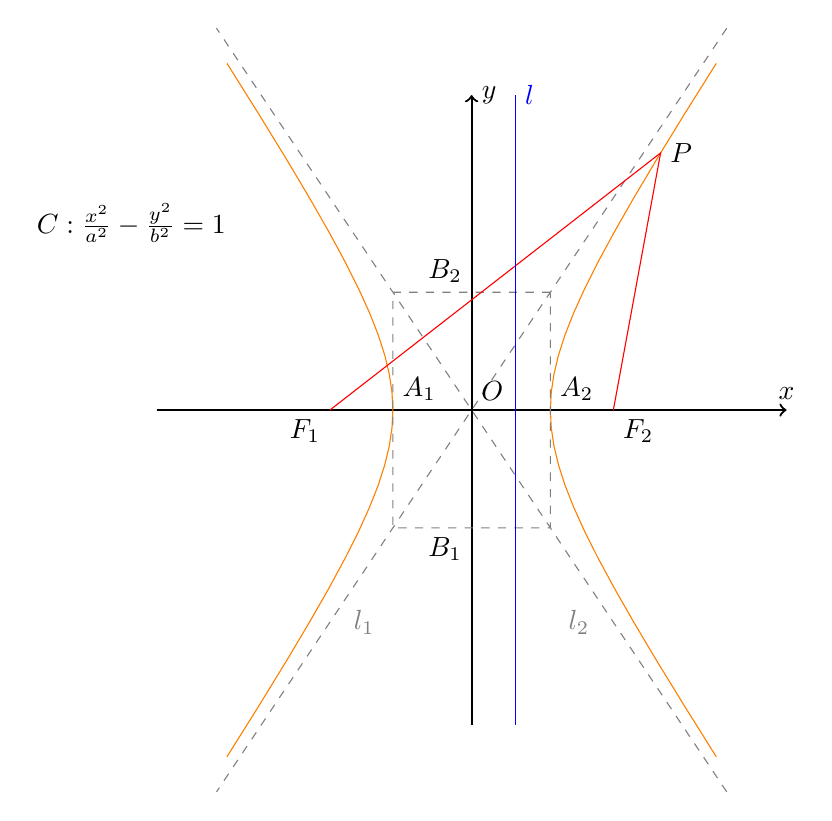
\begin{tikzpicture}
%\draw[gray,help lines,dashed] (-5,-3) grid (5,3);
\draw[thick,->] (-4,0) -- (4,0)node[above]{\(x\)};
\draw[thick,->] (0,-4) -- (0,4)node[right]{\(y\)};
\draw (-3,2)node[above left]{\(C: \frac{x^2}{a^2}-\frac{y^2}{b^2}=1\)};
\pgfmathsetmacro{\e}{1.8}   % eccentricity
\pgfmathsetmacro{\a}{1}
\pgfmathsetmacro{\b}{(\a*sqrt((\e)^2-1)}
\pgfmathsetmacro{\c}{(sqrt((\a)^2+(\b)^2))}
\pgfmathsetmacro{\px}{2.4}
\pgfmathsetmacro{\py}{sqrt(\b^2*(\px^2/\a^2-1))}
\pgfmathsetmacro{\d}{1.8} % 定义域
\draw[orange] plot[domain=-\d:\d] ({\a*cosh(\x)},{\b*sinh(\x)});
\draw[orange] plot[domain=-\d:\d] ({-\a*cosh(\x)},{\b*sinh(\x)});
\pgfmathsetmacro{\k}{1.8*\d}
\coordinate (F1) at (-\c,0);
\coordinate (F2) at (\c,0);
\coordinate (P) at (\px,\py);
\draw[gray,dashed] (\a,\b) -- (-\a,\b) -- (-\a,-\b) -- (\a,-\b) -- (\a,\b)
	(\k*\a,\k*\b) -- (-\k*\a,-\k*\b)
	(\k*\a,-\k*\b) -- (-\k*\a,\k*\b)
	(-\k*\a/2,-\k*\b/2)node[below right]{\(l_1\)}
	(\k*\a/2,-\k*\b/2)node[below left]{\(l_2\)};
\draw[red] (F1)node[below left,black]{\(F_1\)}
	-- (P)node[right,black]{\(P\)}
	-- (F2)node[below right,black]{\(F_2\)};
\pgfmathsetmacro{\dx}{\a^2/\c}
\draw[blue] (\dx,-4) -- (\dx,4)node[right]{\(l\)}; % 准线
\draw (0,0)node[above right]{\(O\)}
	(-\a,0)node[above right]{\(A_1\)}
	(\a,0)node[above right]{\(A_2\)}
	(0,-\b)node[below left]{\(B_1\)}
	(0,\b)node[above left]{\(B_2\)};
\end{tikzpicture}
\caption{双曲线的图形}
\label{figure:解析几何.双曲线的图形}
\end{figure}

我们根据双曲线的标准方程\[
\frac{x^2}{a^2} - \frac{y^2}{b^2} = 1
\]来研究它的几何性质.
\begin{enumerate}
\item 范围

由标准方程可知,双曲线上的点的坐标\((x,y)\)都适合不等式\(\frac{x^2}{a^2}\geq1\),即\(x^2 \geq a^2\),所以\(x \geq a\)或\(x \leq -a\).这说明双曲线在两条直线\(x = \pm a\)的外侧.

\item 对称性

双曲线关于每条坐标轴和原点都是对称的.这时,坐标轴是双曲线的对称轴,原点是双曲线的对称中心.双曲线的对称中心叫做双曲线的\DefineConcept{中心}.

\item 顶点

在标准方程中,令\(y=0\),得\(x = \pm a\),因此双曲线和\(x\)轴有两个交点\(A_1(-a,0)\)、\(A_2(a,0)\).因为\(x\)轴是双曲线的对称轴,所以双曲线和它的对称轴有两个焦点,它们叫做双曲线的\DefineConcept{顶点}.

令\(x=0\),得\(y^2=-b^2\),这个方程没有实数根,说明双曲线和\(y\)轴没有交点,但我们也把\(B_1(0,-b)\)和\(B_2(0,b)\)画在\(y\)轴上.

线段\(A_1 A_2\)叫做双曲线的\DefineConcept{实轴},它的长等于\(2a\),\(a\)叫做双曲线的实半轴长.
线段\(B_1 B_2\)叫做双曲线的\DefineConcept{虚轴},它的长等于\(2b\),\(b\)叫做双曲线的虚半轴长.

\item 渐近线

经过\(A_2\)、\(A_1\)作\(y\)轴的平行线\(x = \pm a\),经过\(B_2\)、\(B_1\)作\(x\)轴的平行线\(y = \pm b\),四条直线围成一个矩形.矩形的两条对角线所在的直线是\(y = \pm\frac{b}{a}x\).可以看出,双曲线的各支向外延伸时,与这两条直线逐渐接近.我们把这两条直线叫做双曲线的\DefineConcept{渐近线}.

在方程\(\frac{x^2}{a^2}-\frac{y^2}{b^2}=1\)中,如果\(a=b\),那么双曲线方程为\(x^2-y^2=a^2\),它的实轴和虚轴的长都等于\(2a\).这时,四条直线\(x=\pm a\)、\(y=\pm a\)围成正方形;渐近线方程成为\(x=\pm y\),它们互相垂直,并且平分双曲线实轴与虚轴所成的角.像这样,实轴和虚轴等长的双曲线叫做\DefineConcept{等轴双曲线}.

\item 离心率

双曲线的焦距与实轴的比\(e = \frac{c}{a}\),叫做双曲线的\DefineConcept{离心率}.因为\(c > a\),所以双曲线的离心率\(e > 1\).

由等式\(c^2-a^2=b^2\)可得\[
\frac{b}{a} = \frac{\sqrt{c^2-b^2}}{a} = \sqrt{\frac{c^2}{a^2}-1} = \sqrt{e^2-1}.
\]因此\(e\)越大,\(\frac{b}{a}\)也越大,即渐近线\(y = \pm\frac{b}{a}x\)的斜率的绝对值越大,这时双曲线的形状就从褊狭逐渐变得开阔.由此可知,双曲线的离心率越大,它的开口就越开阔.
\end{enumerate}

\begin{example}
以已知双曲线的虚轴为实轴,实轴为虚轴的双曲线叫做原双曲线的\DefineConcept{共轭双曲线}.求证:\begin{enumerate}
\item 双曲线和它的共轭双曲线有共同的渐近线;
\item 双曲线和它的共轭双曲线的四个焦点在同一个圆上.
\end{enumerate}
\begin{proof}
设已知双曲线的方程是\[
	\frac{x^2}{a^2}-\frac{y^2}{b^2}=1.
\]
它的焦点坐标为\(F_1(-c,0)\)和\(F_2(c,0)\)
(\(c^2=a^2+b^2\)).
它的渐近线方程是\(y=\pm\frac{b}{a}x\).

根据定义,其共轭双曲线的方程是\[
\frac{y^2}{a^2}-\frac{x^2}{b^2}=1.
\]它的交点坐标为\(F'_1(0,-c)\)和\(F'_2(0,c)\),
可见四个焦点都在圆\(x^2+y^2=c^2\)上.
它的共轭双曲线的渐近线方程是\(x=\pm\frac{a}{b}y\),
也即\(y=\pm\frac{b}{a}x\),
所以双曲线和它的共轭双曲线具有共同的渐近线.
\end{proof}
\end{example}

\begin{example}
点\(P(x,y)\)与定点\(F(c,0)\)的距离和它到定直线\(l: x = \frac{a^2}{c}\)的距离的比是常数\(\frac{c}{a}\)
(\(c > a > 0\)).
求点\(P\)的轨迹.
\begin{solution}
设点\(P\)到直线\(l\)的距离是\(d\),那么所求轨迹就是点集\[
\Set*{ P \given \frac{\abs{PF}}{d} = \frac{c}{a} },
\]由此得\[
\frac{\sqrt{(x-c)^2+y^2}}{\abs{\frac{a^2}{c}-x}} = \frac{c}{a},
\]化简得\[
(c^2-a^2)x^2 - a^2 y^2 = a^2(c^2-a^2).
\]设\(b^2=c^2-a^2\),则可将上式进一步化简为\[
\frac{x^2}{a^2}-\frac{y^2}{b^2}=1.
\]这是双曲线的标准方程,所以点\(P\)的轨迹是双曲线.
\end{solution}

由上例可知,点\(P\)与一个定点的距离和它到一条定直线的距离的比是常数
\(e = \frac{c}{a} > 1\)时,
这个点的轨迹是双曲线.
定点是双曲线的焦点,定直线叫做双曲线的\DefineConcept{准线},常数\(e\)是双曲线的离心率.

对于双曲线\(\frac{x^2}{a^2}-\frac{y^2}{b^2}=1\),相应于焦点\(F(c,0)\)的准线方程是\[
x = \frac{a^2}{c}
\quad\text{或}\quad
x = \frac{a}{e}.
\]根据双曲线的对称性,相应于焦点\(F'(-c,0)\)的准线方程是\(x=-\frac{a^2}{c}\),所以双曲线有两条准线.
\end{example}

\begin{example}
证明:等轴双曲线的离心率是\(\sqrt2\).
\begin{proof}
由定义,等轴双曲线\(x^2-y^2=a^2\)的实半轴长与虚半轴长相等,即\(a=b>0\),故\(c^2 = a^2 + b^2 = 2 a^2\),\(c = \sqrt2 a\),那么等轴双曲线的离心率为\[
e = \frac{c}{a} = \frac{\sqrt2 a}{a} = \sqrt2.
\qedhere
\]
\end{proof}
\end{example}

\begin{example}
证明:从双曲线的一个焦点到一条渐近线的距离等于虚半轴长.
\begin{proof}
设双曲线方程为\[
	\frac{x^2}{a^2}-\frac{y^2}{b^2}=1,
\]
它的右焦点为\(F(c,0)\)
(\(c^2=a^2+b^2\)),
其中一条渐近线为\(y=\frac{b}{a}x\)或\(bx-ay=0\).
由点到直线的距离公式,焦点\(F\)到上述渐近线的距离为\[
	d = \frac{\abs{b \cdot c - a \cdot 0}}{\sqrt{b^2+(-a)^2}}
	= \frac{bc}{c} = b.
	\qedhere
\]
\end{proof}
\end{example}

\begin{example}
已知双曲线\[
C: \frac{x^2}{a^2} - \frac{y^2}{b^2} = 1 \quad(a>b>1).
\]求双曲线在其上任意一点\(P_0(x_0,y_0)\)处的切线方程.
\begin{solution}
因为点\(P_0(x_0,y_0)\)在双曲线\(C\)上,所以\[
\frac{x_0^2}{a^2} - \frac{y_0^2}{b^2} = 1
\quad\text{即}\quad
b^2 x_0^2 - a^2 y_0^2 = a^2 b^2.
\]

当切线\(l\)与\(x\)轴相垂直时,显然只有\((-a,0)\)和\((a,0)\)两点可能是切点,
而它们各自的切线方程分别为\(x=-a\)和\(x=a\).

当切线\(l\)不与\(x\)轴相垂直时,
设切线方程为\(l: y = kx + p\),其中\(p = y_0 - k x_0\).
联立方程组,得\[
\begin{cases}
y = kx + p, \\
\frac{x^2}{a^2} - \frac{y^2}{b^2} = 1.
\end{cases}
\]那么有\[
\frac{1}{a^2} x^2 - \frac{1}{b^2} (kx+p)^2 = 1,
\]\[
b^2 x^2 - a^2 (k^2 x^2 + 2kpx + p^2) = a^2 b^2,
\]\[
(b^2 - a^2 k^2) x^2 - 2 a^2 k p x - a^2 (p^2 + b^2) = 0.
\]令判别式\(\Delta_1 = (2 a^2 k p)^2 + 4 (b^2 - a^2 k^2) a^2 (p^2 + b^2) = 0\),得\[
4 a^4 k^2 p^2 = 4 (a^2 k^2 - b^2) a^2 (p^2 + b^2),
\]\[
a^2 k^2 p^2 = (a^2 k^2 - b^2)(p^2 + b^2),
\]\[
a^2 b^2 k^2 = b^2(p^2 + b^2),
\]\[
a^2 k^2 = p^2 + b^2,
\]
代入\(p = y_0 - k x_0\),得\[
a^2 k^2 = (y_0 - k x_0)^2 + b^2,
\]\[
y_0^2 - 2k x_0 y_0 + k^2 x_0^2 + b^2 = a^2 k^2,
\]\[
(x_0^2 - a^2) k^2 - 2 x_0 y_0 k + (y_0^2 + b^2) = 0.
\]上式的判别式\(\Delta_2 = (2 x_0 y_0)^2 - 4(x_0^2 - a^2)(y_0^2 + b^2)
= 4(a^2 b^2 + a^2 y_0^2 - b^2 x_0^2) = 0\),故可解得\[
k = \frac{2 x_0 y_0}{2 (x_0^2 - a^2)}
= \frac{x_0 y_0}{x_0^2 - a^2}.
\]那么\(l\)的方程为\[
y - y_0 = \frac{x_0 y_0}{x_0^2 - a^2} (x - x_0),
\]\[
(x_0^2 - a^2) y = x_0 y_0 x + (x_0^2 - a^2) y_0 - x_0^2 y_0
= x_0 y_0 x - a^2 y_0,
\]\[
x_0 y_0 x + (a^2 - x_0^2) y = a^2 y_0,
\]\[
\frac{x_0 x}{a^2} + (a^2 - x_0^2) \frac{y_0 y}{a^2 y_0^2} = 1,
\]\[
\frac{x_0 x}{a^2} + (a^2 - x_0^2) \frac{y_0 y}{(x_0^2 - a^2) b^2} = 1,
\]最后化简得\begin{equation}\label{equation:解析几何.双曲线的切线}
\frac{x_0 x}{a^2} - \frac{y_0 y}{b^2} = 1.
\end{equation}
这就是双曲线在其上任意一点\(P_0(x_0,y_0)\)处的切线方程.
\end{solution}
\end{example}

\begin{theorem}[双曲线的焦点三角形]
设\(P\)是双曲线\(C: \frac{x^2}{a^2} - \frac{y^2}{b^2} = 1\ (a>0,b>0)\)上任一点,
\(F_1\)、\(F_2\)是\(C\)的焦点,那么\[
S_{\triangle P F_1 F_2} = \frac{b^2}{\tan(\theta/2)},
\]其中\(\theta=\angle{F_1 P F_2}\).
\end{theorem}

\subsection{抛物线}
\begin{definition}
在平面内,与一个定点和一条定直线的距离相等的点的集合,
叫做\DefineConcept{抛物线}(parabola).
这个定点叫做抛物线的\DefineConcept{焦点}.
这条定直线叫做抛物线的\DefineConcept{准线}.
\end{definition}

取经过焦点\(F\)且垂直于准线\(l\)的直线为\(x\)轴,\(x\)轴于\(l\)相交于点\(K\),以线段\(KF\)的垂直平分线为\(y\)轴.设\(\abs{KF}=p\),
那么,焦点\(F\)的坐标为\((\frac{p}{2},0)\),准线\(l\)的方程为\(x=-\frac{p}{2}\).

设抛物线上的点\(P(x,y)\)到\(l\)的距离为\(d\).抛物线就是点集\[
\Set*{ P \given \abs{PF} = d }.
\]因为\(\abs{PF} = \sqrt{\left(x-\frac{p}{2}\right)^2+y^2}\),\(d = \abs{x+\frac{p}{2}}\),所以\[
\sqrt{\left(x-\frac{p}{2}\right)^2+y^2} = \abs{x+\frac{p}{2}}.
\]将上式两边平方,并化简得\begin{equation}
y^2 = 2px, \quad p > 0.
\end{equation}
这个方程叫做\DefineConcept{抛物线的标准方程},它所表示的抛物线的焦点在\(x\)轴的正半轴上,
坐标是\((\frac{p}{2},0)\),准线方程是\(x=-\frac{p}{2}\).

一条抛物线,由于它在坐标平面上的位置不同,方程也不同,所以抛物线的标准方程还有其他几种形式:\(y^2 = -2px\)、\(x^2 = 2py\)、\(x^2 = -2py\).

\begin{figure}[ht]
\centering
\begin{tikzpicture}
%\draw[gray,help lines,dashed] (-3,-3) grid (3,3);
\draw[thick,->] (-3,0) -> (4,0)node[above]{\(x\)};
\draw[thick,->] (0,-4) -> (0,4)node[right]{\(y\)};
\draw (0,0)node[below left]{\(O\)};
\pgfmathsetmacro{\p}{2}
\pgfmathsetmacro{\x}{3}
\pgfmathsetmacro{\y}{sqrt(2*\p*\x)}
\pgfmathsetmacro{\f}{\p/2}
\coordinate (F)at(\f,0);
\draw[orange] [rotate=-90](0,0)parabola(\y,\x) [rotate=180](0,0)parabola(\y,-\x);
\draw[purple] (-\f,-4)--(-\f,4);
\draw (2,2)node[above right]{\(C: y^2 = 2px\ (p>0)\)}
	(-\f,-1)node[below left]{\(l: x = -\frac{p}{2}\)};
\fill (F)circle(2pt)node[below right]{\(F\)};
\pgfmathsetmacro{\px}{\f/2}
\pgfmathsetmacro{\py}{\p/sqrt(2)}
\coordinate (P)at(\px,\py);
\coordinate (Q)at(-\f,\py);
\coordinate (K)at(-\f,0);
\draw[red] (F)--(P)node[above,black]{\(P\)}--(Q)node[left,black]{\(Q\)}
	pic[draw=gray,-,angle radius=0.3cm]{right angle=P--Q--K};
\draw (K)node[below left]{\(K\)};
\coordinate (M)at(\f,\p);
\coordinate (N)at(\f,-\p);
\draw[blue] (M)node[above,black]{\(M\)}--(N)node[below,black]{\(N\)}
	pic[draw=gray,-,angle radius=0.3cm]{right angle=N--F--K};
\end{tikzpicture}
\caption{抛物线的图形}
\label{figure:解析几何.抛物线的图形}
\end{figure}

我们根据抛物线的标准方程\[
y^2 = 2px, \quad p > 0
\]来研究它的几何性质.
\begin{enumerate}
\item 范围

因为\(p>0\),由标准方程可知,抛物线上的点的坐标\((x,y)\)都适合不等式\(x \geq 0\),所以这条抛物线在\(y\)轴的右侧.当\(x\)的值增大时,\(\abs{y}\)也增大,这说明抛物线向右上方和右下方无限延伸.

\item 对称性

以\(-y\)代\(y\),标准方程形式不变,所以这个抛物线关于\(x\)轴对称,我们把抛物线的对称轴叫做抛物线的\DefineConcept{轴}.

\item 顶点

抛物线和它的轴的交点叫做抛物线的\DefineConcept{顶点}.
在标准方程中,当\(y=0\)时,\(x=0\),因此标准方程所表示的抛物线的顶点就是坐标原点.

\item 离心率

抛物线上的点\(P\)与焦点和准线的距离的比,叫做抛物线的\DefineConcept{离心率},用\(e\)表示.
由抛物线的定义,抛物线的离心率为\(e = 1\).
\end{enumerate}

\begin{example}
已知抛物线方程\(C: y^2=2px\ (p>0)\).
下面讨论过焦点\(F(p/2,0)\)的直线\(l\)与抛物线的交点个数.
\begin{enumerate}
	\item 当直线\(l\)的方程为\(y=0\)时,
	代入抛物线方程得\(2px = 0\),解得\(x=0\).
	可见直线\(l\)与抛物线\(C\)只有一个交点,即坐标原点\(O\).

	\item 当直线\(l\)的方程为\(x=p/2\)时,
	代入抛物线方程得\(y^2=2p\cdot(p/2)=p^2\),解得\(y=\pm p\).
	可见直线\(l\)与抛物线\(C\)有两个交点\(P(p/2,p)\)和\(Q(p/2,-p)\).
	焦点弦长为\(\abs{PQ} = 2p\).

	\begin{center}
		\begin{tikzpicture}
			%\draw[gray,help lines,dashed] (-3,-3) grid (3,3);
			\draw[thick,->] (-2,0) -> (4,0)node[above]{\(x\)};
			\draw[thick,->] (0,-4) -> (0,4)node[right]{\(y\)};
			\draw (0,0)node[below left]{\(O\)};
			\pgfmathsetmacro{\p}{2}  % 参数p
			\pgfmathsetmacro{\x}{3}
			\pgfmathsetmacro{\y}{sqrt(2*\p*\x)}
			\pgfmathsetmacro{\f}{\p/2}  % 焦点横坐标
			\coordinate (F)at(\f,0);
			\coordinate (2F)at(2\f,0);
			\draw[orange] [rotate=-90](0,0)parabola(\y,\x) [rotate=180](0,0)parabola(\y,-\x);
			\draw[purple] (-\f,-4)--(-\f,4); % 准线
			\draw (2,-3)node[above right]{\(C: y^2 = 2px\ (p>0)\)};
			\pgfmathsetmacro{\k}{3}  % 焦点弦 斜率
			\pgfmathsetmacro{\a}{\p/(2*\k^2)}
			\pgfmathsetmacro{\b}{\p/\k}
			\pgfmathsetmacro{\c}{sqrt(\k^2+1)}
			\pgfmathsetmacro{\px}{\a*(\c+1)^2}
			\pgfmathsetmacro{\py}{\b*(\c+1)}
			\pgfmathsetmacro{\qx}{\a*(\c-1)^2}
			\pgfmathsetmacro{\qy}{-\b*(\c-1)}
			\coordinate (P)at(\px,\py);
			\coordinate (Q)at(\qx,\qy);
			\coordinate (P1)at(-\f,\py);
			\coordinate (Q1)at(-\f,\qy);
			\coordinate (K)at(-\f,0);
			\fill (P)circle(2pt)node[below right]{\(P\)}
				(F)circle(2pt)node[below right]{\(F\)}
				(Q)circle(2pt)node[right]{\(Q\)};
			\draw[red] (P)--(P1)node[left,black]{\(P_1\)}
				pic[draw=gray,-,angle radius=0.3cm]{right angle=P--P1--K}
				(Q)--(Q1)node[left,black]{\(Q_1\)}
				pic[draw=gray,-,angle radius=0.3cm]{right angle=Q--Q1--K};
			\draw[blue] (P)--(F)--(Q);
			\draw pic["\(\theta\)",draw=gray,-,angle eccentricity=1.7,angle radius=5mm]{angle=2F--F--P};
		\end{tikzpicture}
	\end{center}

	\item 当直线\(l\)的方程为\(y=k\left(x-\frac{p}{2}\right)\ (k\neq0)\)时,代入抛物线方程得\[
		\left[k \left(x-\frac{p}{2}\right)\right]^2 = 2px,
	\]
	化简得\begin{gather}
		k^2 x^2 - (k^2 + 2)px + \frac{1}{4} k^2 p^2 = 0, \tag1
	\end{gather}
	因为\[
		\Delta = [- (k^2 + 2)p]^2 - 4 k^2 \frac{1}{4} k^2 p^2
		= 4 p^2 (k^2 + 1) > 0,
	\]
	所以(1)式总有两个实根\[
		x_{1,2} = \frac{(k^2+2)p \pm \sqrt\Delta}{2 k^2}
		= \frac{p}{2 k^2} (\sqrt{k^2+1} \pm 1)^2.
	\]
	可见直线\(l\)与抛物线\(C\)有两个交点\(P(x_1,y_1)\)和\(Q(x_2,y_2)\).
	不妨设\(x_1 > x_2\),即\[
		x_1 = \frac{(k^2+2)p + \sqrt\Delta}{2 k^2}
		= \frac{p}{2 k^2} (\sqrt{k^2+1} + 1)^2,
	\]\[
		x_2 = \frac{(k^2+2)p - \sqrt\Delta}{2 k^2}
		= \frac{p}{2 k^2} (\sqrt{k^2+1} - 1)^2.
	\]
	将\(x_{1,2}\)代入抛物线方程得\[
		y^2 = 2 p^2 \frac{(\sqrt{k^2+1}\pm1)^2}{2 k^2}
		= \frac{p^2}{k^2} (\sqrt{k^2+1}\pm1)^2,
	\]\[
		y = \pm \frac{p}{k} (\sqrt{k^2+1}\pm1).
	\]
	当\(k>0\)时,由\(x_1 > x_2\)可知\(y_1 > 0 > y_2\),那么\[
		y_1 = \frac{p}{k} (\sqrt{k^2+1}+1),
		\qquad
		y_2 = -\frac{p}{k} (\sqrt{k^2+1}-1).
	\]
	由两点间距离公式,焦点弦长为\begin{equation}
		\abs{PQ} = \sqrt{
		\left(\frac{p}{2 k^2} \cdot 4 \sqrt{k^2+1}\right)^2
		+\left(\frac{p}{k} \cdot 2 \sqrt{k^2+1}\right)^2
		} = 2p \left(1+\frac{1}{k^2}\right).
	\end{equation}
	若记\(k=\tan\theta\),则上述弦长公式也可改写为\begin{equation}
		\abs{PQ} = 2p \frac{\tan^2\theta+1}{\tan^2\theta}
		= 2p \frac{\sec^2\theta}{\tan^2\theta}
		= 2p \frac{1}{\sin^2\theta}
		= 2p \csc^2\theta.
	\end{equation}

	现在我们来检验上述弦长公式的正确性.
	根据抛物线的定义,抛物线上一点到焦点与其到准线的距离相等,
	故\(\abs{PF} = \abs{P P_1} = x_1 + \frac{p}{2}\),
	\(\abs{QF} = \abs{Q Q_1} = x_2 + \frac{p}{2}\),
	那么\(\abs{PQ} = \abs{PF}+\abs{QF} = x_1 + x_2 + p\).
	代入\(x_{1,2}\),得\begin{align*}
		\abs{PQ} &= \frac{p}{2 k^2} \left[(\sqrt{k^2+1} + 1)^2 + (\sqrt{k^2+1} - 1)^2\right] + p \\
		&= p\left[\frac{2(k^2 + 1) + 2}{2 k^2} + 1\right]
		= p \frac{4k^2 + 4}{2k^2}
		= 2p \left(1+\frac{1}{k^2}\right).
	\end{align*}
\end{enumerate}

另外,可以注意到,\(P\)、\(Q\)两点的坐标满足\begin{equation}
	x_1 \cdot x_2 = \frac{p^2}{4},
	\qquad
	y_1 \cdot y_2 = -p^2.
\end{equation}

\(P\)、\(Q\)两点的焦半径\(\abs{FP}\)、\(\abs{FQ}\)满足\begin{equation}
	\frac{1}{\abs{FP}} + \frac{1}{\abs{FB}}
	= \frac{2}{p}.
\end{equation}
\end{example}


\section{常见曲面}
本章将介绍一些常见曲面,
一方面了解如何利用曲面的几何特性建立它的方程,
另一方面熟悉如何利用方程研究曲面的几何性质.

\subsection{球面和旋转面}
\subsubsection{球面的一般方程}
我们来求球心为\(M_0(x_0,y_0,z_0)\),半径为\(R\)的球面的方程.
点\(M(x,y,z)\)在这个球面上的充分必要条件是\(\abs{\vec{M_0 M}} = R\),即
\begin{equation}\label{equation:解析几何.球面的标准方程}
	(x-x_0)^2+(y-y_0)^2+(z-z_0)^2=R^2,
\end{equation}
展开得
\begin{equation}\label{equation:解析几何.球面的一般方程}
	x^2 + y^2 + z^2 + 2 b_1 x + 2 b_2 y + 2 b_3 z + c = 0,
\end{equation}
其中\(b_1 = -x_0\),
\(b_2 = -y_0\),
\(b_3 = -z_0\),
\(c = x_0^2 + y_0^2 + z_0^2 - R^2\).

\cref{equation:解析几何.球面的标准方程}
和\cref{equation:解析几何.球面的一般方程}
就是所求球面的方程,
它是一个三元二次方程,
没有交叉项(即含\(xy,xz,yz\)的项),
平方项的系数相同.
反之,任一形如\cref{equation:解析几何.球面的一般方程} 的方程也可经过配方得到
\begin{equation}\label{equation:解析几何.形如球面的一般方程的方程经过配方所得方程}
	(x+b_1)^2 + (y+b_2)^2 + (z+b_3)^2 + (c-b_1^2-b_2^2-b_3^2) = 0.
\end{equation}
当\(b_1^2+b_2^2+b_3^2>c\)时,
\cref{equation:解析几何.形如球面的一般方程的方程经过配方所得方程}
表示一个球心在\((-b_1,-b_2,-b_3)\),半径为\(\sqrt{b_1^2+b_2^2+b_3^2-c}\)的球面;
当\(b_1^2+b_2^2+b_3^2=c\)时,
它表示一个点\((-b_1,-b_2,-b_3)\);
当\(b_1^2+b_2^2+b_3^2<c\)时,
它没有轨迹(或者说它表示一个虚球面).

\subsubsection{球面的参数方程,点的球面坐标}
如果球心在原点,半径为\(R\),在球面上任取一点\(M(x,y,z)\),
从\(M\)作\(Oxy\)平面的垂线,垂足为\(N\),
连接\(OM,ON\),
设\(x\)轴的正半轴到\(\vec{ON}\)的角度为\(\phi\),
\(\vec{ON}\)到\(\vec{OM}\)的角度为\(\theta\)
(\(M\)在\(Oxy\)平面上方时,\(\theta>0\);否则\(\theta<0\)),
则有
\begin{equation}\label{equation:解析几何.球心在原点半径为R的球面的参数方程}
	\left\{ \begin{array}{l}
		x = R \cos\theta \cos\phi, \\
		y = R \cos\theta \sin\phi, \\
		z = R \sin\theta,
	\end{array} \right.
	\quad
	-\frac{\pi}{2} \leq \theta \leq \frac{\pi}{2},
	-\pi < \phi \leq \pi.
\end{equation}
\cref{equation:解析几何.球心在原点半径为R的球面的参数方程}
称为“球心在原点、半径为R的球面的\DefineConcept{参数方程}”;
它有两个参数\(\theta,\phi\),
其中\(\theta\)称为\DefineConcept{纬度},
\(\phi\)称为\DefineConcept{经度}.
球面上的每一个点(除去它与\(z\)轴的交点)对应唯一的实数对\((\theta,\phi)\),
因此\((\theta,\phi)\)称为“球面上的点的\DefineConcept{曲纹坐标}”.

因为几何空间中任一点\(M(x,y,z)\)必在以原点为球心,yi
以\(R=\abs{\vec{OM}}\)为半径的球面上,
而球面上的点(除去它与\(z\)轴的交点外)
又由它的曲纹坐标\((\theta,\phi)\)唯一确定,
因此,除去\(z\)轴外,几何空间中的点\(M\)由有序三元实数组\((R,\theta,\phi)\)唯一确定.
我们把\((R,\theta,\phi)\)称为“几何空间中的点的\DefineConcept{球面坐标}或\DefineConcept{空间极坐标}”,
其中\[
	R \geq 0,
	\qquad
	-\frac{\pi}{2} \leq \theta \leq \frac{\pi}{2},
	\qquad
	-\pi < \phi \leq \pi.
\]

\subsubsection{曲面和曲线的一般方程、参数方程}
从球面的方程 \labelcref{equation:解析几何.球面的一般方程}
和球面的参数方程 \labelcref{equation:解析几何.球心在原点半径为R的球面的参数方程} 看到,
一般来说,曲面的一般方程是一个三元方程
\begin{equation}\label{equation:解析几何.曲面的一般方程}
	F(x,y,z) = 0,
\end{equation}
曲面的参数方程是含两个参数的方程
\begin{equation}\label{equation:解析几何.曲面的参数方程}
	\left\{ \begin{array}{l}
		x = x(u,v), \\
		y = y(u,v), \\
		z = z(u,v),
	\end{array} \right.
	\quad
	a \leq u \leq b,
	c \leq v \leq d.
\end{equation}
对于\((u,v)\)的每一对值,
由方程 \labelcref{equation:解析几何.曲面的参数方程} 确定的点\((x,y,z)\)都在此曲面上;
而此曲面上任一点的坐标都可由\((u,v)\)的某一对值
通过方程 \labelcref{equation:解析几何.曲面的参数方程} 表示.
于是,通过曲面的参数方程 \labelcref{equation:解析几何.曲面的参数方程},
曲面上的点(可能要除去个别点)便可由数对\((u,v)\)来确定,
于是称\((u,v)\)为“曲面上的点的\DefineConcept{曲纹坐标}”.

我们可以给出如下定义.
\begin{definition}
如果曲面\(S\)与三元方程\[
	F(x,y,z)=0
\]满足
\begin{enumerate}
	\item 曲面\(S\)上任一点的坐标都满足这个三元方程,
	\item 不在曲面\(S\)上的点的坐标都不满足这个三元方程,
\end{enumerate}
那么,方程\(F(x,y,z)=0\)就叫做“曲面\(S\)的\DefineConcept{方程}”,
而曲面\(S\)就叫做“方程\(F(x,y,z)=0\)的\DefineConcept{图形}”.
\end{definition}

由于几何空间中曲线可以看成两个曲面的交线,
所以它的一般方程就是联立两个三元方程所得的方程组\begin{equation}\label{equation:解析几何.曲线的一般方程}
	\left\{ \begin{array}{l}
		F(x,y,z) = 0, \\
		G(x,y,z) = 0;
	\end{array} \right.
\end{equation}
而它的参数方程则是含有一个参数的方程
\begin{equation}\label{equation:解析几何.曲线的参数方程}
	\left\{ \begin{array}{l}
		x = x(t), \\
		y = y(t), \\
		z = z(t),
	\end{array} \right.
	\quad
	a \leq t \leq b.
\end{equation}
对于\(t\)的每一个值,
由方程 \labelcref{equation:解析几何.曲线的参数方程} 确定的点\((x,y,z)\)都在此曲线上;
而此曲线上任一点的坐标都可由\(t\)的某个值
通过方程 \labelcref{equation:解析几何.曲线的参数方程} 表示.

\subsubsection{旋转面}
球面可以看成一个半圆绕它的直径旋转一周所形成的曲面.
现在来研究更一般的情形.

我们称一条曲线\(\Gamma\)绕一条直线\(l\)旋转所得的曲面为\DefineConcept{旋转面},
其中\(l\)称为\DefineConcept{轴},\(\Gamma\)称为\DefineConcept{母线}.

母线\(\Gamma\)上的任一点\(M_0\)绕\(l\)旋转会得到一个圆,我们称之为\DefineConcept{纬圆}.
纬圆所在的平面与轴\(l\)垂直.
过\(l\)的半平面与旋转面的交线称为\DefineConcept{经线}.
经线可以作为母线,但母线不一定是经线.

已知轴\(l\)经过点\(M_1(x_1,y_1,z_1)\),
方向向量为\(\vb{\nu}=(A,B,C)\),
母线\(\Gamma\)的方程为\[
	\left\{ \begin{array}{l}
		F(x,y,z) = 0, \\
		G(x,y,z) = 0.
	\end{array} \right.
\]
点\(M(x,y,z)\)在旋转面上的充分必要条件是
\(M\)在经过母线\(\Gamma\)上某一点\(M_0(x_0,y_0,z_0)\)的纬圆上,
即有母线\(\Gamma\)上的一点\(M_0\),
使得\(M\)和\(M_0\)到轴\(l\)的距离相等
(或到轴上一点\(M_1\)的距离相等),
并且\(\vec{M_0 M} \perp l\).
因此有\[
	\left\{ \begin{array}{l}
		F(x_0,y_0,z_0) = 0, \\
		G(x_0,y_0,z_0) = 0, \\
		\abs{\vec{M M_1} \times \vb{\nu}} = \abs{\vec{M_0 M_1} \times \vb{\nu}}, \\
		A(x-x_0) + B(y-y_0) + C(z-z_0) = 0.
	\end{array} \right.
\]
从这个方程组中消去参数\(x_0,y_0,z_0\),就得到关于\(x,y,z\)的方程,它就是所求旋转面的方程.

现在设旋转面的轴是\(z\)轴,
母线\(\Gamma\)在\(Oyz\)平面上,
其方程为\[
	\left\{ \begin{array}{l}
		f(y,z) = 0, \\
		x = 0,
	\end{array} \right.
\]
则点\(M(x,y,z)\)在旋转面上的充分必要条件是\[
	\left\{ \begin{array}{l}
		f(y_0,z_0) = 0, \\
		x_0 = 0, \\
		x^2+y^2=x_0^2+y_0^2, \\
		1\cdot(z-z_0) = 0.
	\end{array} \right.
\]
消去参数\(x_0,y_0,z_0\),得
\begin{equation}\label{equation:解析几何.Oyz平面上的曲线绕z轴旋转所得旋转面的方程}
	f(\pm\sqrt{x^2+y^2},z) = 0.
\end{equation}
\cref{equation:解析几何.Oyz平面上的曲线绕z轴旋转所得旋转面的方程} 就是所求旋转面的方程.
由此可见,为了得到由\(Oyz\)平面上的曲线\(\Gamma\)绕\(z\)轴旋转所得旋转面的方程,
只要将母线\(\Gamma\)在\(Oyz\)平面上的方程中的\(y\)改为\(\pm\sqrt{x^2+y^2}\),保持\(z\)不变.
坐标平面上的曲线绕坐标轴旋转所得旋转面的方程都有类似的规律.

\begin{table}[ht]
	\centering
	\begin{tabular}{|c|c|c|}
	\hline
	曲线方程 & 旋转轴 & 旋转曲面方程 \\ \hline
	\multirow{2}{*}{\(f(x,y)=0\)} & \(x\) & \(f(x,\pm\sqrt{y^2+z^2})=0\) \\ \cline{2-3}
		& \(y\) & \(f(\pm\sqrt{x^2+z^2},y)=0\) \\ \hline
	\multirow{2}{*}{\(f(y,z)=0\)} & \(y\) & \(f(y,\pm\sqrt{x^2+z^2})=0\) \\ \cline{2-3}
		& \(z\) & \(f(\pm\sqrt{x^2+y^2},z)=0\) \\ \hline
	\multirow{2}{*}{\(f(x,z)=0\)} & \(x\) & \(f(x,\pm\sqrt{y^2+z^2})=0\) \\ \cline{2-3}
		& \(z\) & \(f(\pm\sqrt{x^2+y^2},z)=0\) \\
	\hline
	\end{tabular}
	\caption{}
\end{table}


\begin{example}
母线\[
	\Gamma: \left\{ \begin{array}{l}
		y^2 = 2pz, \\
		x = 0,
	\end{array} \right.
	\quad p>0
\]
绕\(z\)轴旋转所得旋转面的方程为\[
	x^2+y^2=2pz.
\]
这个曲面称为\DefineConcept{旋转抛物面}.
\end{example}

\begin{example}
母线\[
	\Gamma: \left\{ \begin{array}{l}
		\frac{x^2}{a^2}-\frac{y^2}{b^2}=1, \\
		z=0
	\end{array} \right.
\]
绕\(x\)旋转所得旋转面的方程为\[
	\frac{x^2}{a^2}-\frac{y^2+z^2}{b^2}=1.
\]
这个曲面称为\DefineConcept{旋转双叶双曲面}.

母线\(\Gamma\)绕\(y\)轴旋转所得旋转面的方程为\[
	\frac{x^2+z^2}{a^2}-\frac{y^2}{b^2}=1.
\]
这个曲面称为\DefineConcept{旋转单叶双曲面}.
\end{example}

\begin{example}
圆\[
	\left\{ \begin{array}{l}
		(x-a)^2+z^2=r^2, \\
		y=0,
	\end{array} \right.
	\quad 0<r<a
\]
绕\(z\)轴旋转所得旋转面的方程为\[
	(\pm\sqrt{x^2+y^2}-a)^2+z^2=r^2,
\]
即\[
	(x^2+y^2+z^2+a^2-r^2)^2=4a^2(x^2+y^2).
\]
这个曲面称为\DefineConcept{环面}.
\end{example}

\subsection{柱面和锥面}
\subsubsection{柱面方程的建立}
一条直线\(l\)沿着一条空间曲线\(C\)平行移动时所形成的曲面称为\DefineConcept{柱面},
其中\(l\)称为\DefineConcept{母线},\(C\)称为\DefineConcept{准线}.

由于平面可以看成是由一条直线沿着另一条与之相交的直线平行移动所形成的,故平面也是柱面.

对于任意一个柱面,它的准线和母线都不唯一.
但是,除去平面以外,任意柱面的母线方向是唯一的.
与每一条母线都相交的曲线均可作为准线.

设一个柱面的母线方向为\(\vb{\nu}=(A,B,C)\),
准线的方程为\[
	\left\{ \begin{array}{l}
		F(x,y,z) = 0, \\
		G(x,y,z) = 0.
	\end{array} \right.
\]
我们来求这个柱面的方程.

点\(M(x,y,z)\)在此柱面上的充分必要条件是\(M\)在某一条母线上,
即有准线\(C\)上一点\(M_0(x_0,y_0,z_0)\),
使得\(M\)在经过\(M_0\)且方向向量为\(\vb{\nu}\)的直线上.
因此有\[
	\left\{ \begin{array}{l}
		F(x_0,y_0,z_0) = 0, \\
		G(x_0,y_0,z_0) = 0, \\
		x = x_0 + Au, \\
		y = y_0 + Bu, \\
		z = z_0 + Cu.
	\end{array} \right.
\]
消去\(x_0,y_0,z_0\),得\[
	\left\{ \begin{array}{l}
		F(x - Au,y - Bu,z - Cu) = 0, \\
		G(x - Au,y - Bu,z - Cu) = 0.
	\end{array} \right.
\]
再消去参数\(u\),得到关于\(x,y,z\)的一个方程,
它就是所求柱面的方程.

如果给定的准线\(C\)的方程是一个参数方程\[
	\left\{ \begin{array}{l}
		x = f(t), \\
		y = g(t), \\
		z = h(t),
	\end{array} \right.
	\quad a \leq t \leq b,
\]
则同理可得柱面的参数方程为\[
	\left\{ \begin{array}{l}
		x = f(t) + Au, \\
		y = g(t) + Bu, \\
		z = h(t) + Cu,
	\end{array} \right.
	\quad
	a \leq t \leq b,
	-\infty < u < +\infty.
\]

\subsubsection{圆柱面,点的柱面坐标}
现在来看圆柱面的方程.
圆柱面有一条对称轴\(l\),
圆柱面上每一个点到轴\(l\)的距离都相等,
这个距离称为圆柱面的半径.
圆柱面的准线可取成一个圆\(C\),
它的母线方向与准线圆垂直.
如果知道准线圆的方程和母线方向,
则可用前一目中所述的方法求出圆柱面的方程.
如果知道圆柱面的半径为\(r\),母线方向为\(\vb{\nu}=(A,B,C)\),
以及圆柱面的对称轴\(l\)经过点\(M_0(x,y,z)\),
则点\(M(x,y,z)\)在此圆柱面上充分必要条件是\(M\)到轴\(l\)的距离等于\(r\),即\[
	\frac{\abs{\vec{M M_0} \times \vb{\nu}}}{\abs{\vb{\nu}}} = r.
\]
由此出发可求得圆柱面的方程.
特别地,设圆柱面的对称轴为\(z\)轴,
则这个圆柱面的方程为
\begin{equation}\label{equation:解析几何.以z轴为对称轴r为半径的圆柱面的一般方程}
	x^2+y^2=r^2.
\end{equation}

由于几何空间中任意一点\(M(x,y)\)
必在以\(r=\sqrt{x^2+y^2}\)为半径,
\(z\)轴为对称轴的圆柱面上,xi
显然这个圆柱面的参数方程为\[
	\left\{ \begin{array}{l}
		x = r \cos\theta, \\
		y = r \sin\theta, \\
		z = u,
	\end{array} \right.
	\quad 0\leq \theta < 2\pi,
	-\infty < u < +\infty.
\]
因此,圆柱面上的点\(M\)可以由数对\((\theta,u)\)所确定,
从而几何空间中任意一点\(M\)被有序三元实数组\((r,\theta,u)\)所确定.
\((r,\theta,u)\)称为点\(M\)的\DefineConcept{柱面坐标}.

\subsubsection{柱面方程的特点}
从\cref{equation:解析几何.以z轴为对称轴r为半径的圆柱面的一般方程} 看到,
母线平行于\(z\)轴的圆柱面的方程中不含\(z\),或者说\(z\)的系数为零.
这个结论对于一般的柱面也成立.
\begin{theorem}
%@see: 《解析几何》(丘维声) P86 定理2.1
若一个柱面的母线平行于\(x\)轴,则它的方程中不含\(x\);
若它的母线平行于\(y\)轴,则它的方程中不含\(y\);
若它的母线平行于\(z\)轴,则它的方程中不含\(z\).
反之,若一个三元方程不含\(x\),则它一定表示一个母线平行于\(x\)轴的柱面;
若这个方程不含\(y\),则它一定表示一个母线平行于\(y\)轴的柱面;
若这个方程不含\(z\),则它一定表示一个母线平行于\(z\)轴的柱面.
\begin{proof}
设一个柱面的母线平行于\(z\)轴,则这个柱面的每条母线必与\(Oxy\)平面相交,
从而这个柱面与\(Oxy\)平面的交线\(C\)可以作为准线.
设\(C\)的方程是\[
	\left\{ \begin{array}{l}
		f(x,y) = 0, \\
		z = 0.
	\end{array} \right.
\]
点\(M\)在此柱面上的充分必要条件是:
存在准线\(C\)上一点\(M_0(x_0,y_0,z_0)\),
使得\(M\)在经过\(M_0\)且方向向量为\(\vb{\nu}=(0,0,1)\)的直线上.
因此有\[
	\left\{ \begin{array}{l}
		f(x_0,y_0) = 0, \\
		z_0 = 0, \\
		x = x_0, \\
		y = y_0, \\
		z = z_0 + u.
	\end{array} \right.
\]
消去\(x_0,y_0,z_0\),得\[
	\left\{ \begin{array}{l}
		f(x,y) = 0, \\
		z = u.
	\end{array} \right.
\]
由于参数可以取任意实数值,于是得到这个柱面的方程为\[
	f(x,y) = 0.
\]

反之,任给一个不含\(z\)的三元方程\(g(x,y)=0\),我们考虑以曲线\[
	D: \left\{ \begin{array}{l}
		g(x,y) = 0, \\
		z = 0
	\end{array} \right.
\]
为准线,\(z\)轴方向为母线方向的柱面.
由上述讨论可知,这个柱面的方程为\(g(x,y)=0\).
因此,方程\(g(x,y)=0\)表示一个母线平行于\(z\)轴的柱面.

母线平行于\(x\)轴和\(y\)轴的情形可以类似讨论.
\end{proof}
\end{theorem}

\begin{example}
方程\[
	\frac{x^2}{a^2} + \frac{y^2}{b^2} - 1 = 0
\]
表示母线平行于\(z\)轴的柱面,它与\(Oxy\)平面的交线为\[
	\left\{ \begin{array}{l}
		\frac{x^2}{a^2} + \frac{y^2}{b^2} = 1, \\
		z = 0.
	\end{array} \right.
\]
这条交线是椭圆,因而这个柱面称为\DefineConcept{椭圆柱面}.

类似地,方程\[
	\frac{x^2}{a^2} - \frac{y^2}{b^2} + 1 = 0
\]
表示母线平行于\(z\)轴的双曲柱面;
方程\[
	x^2 + 2py = 0
	\quad(p>0)
\]
表示母线平行于\(z\)轴的抛物柱面.
\end{example}

\subsubsection{锥面方程的建立}
在几何空间中,由曲线\(C\)上的点
与不在\(C\)上的一个定点\(M_0\)的连线组成的曲面称为\DefineConcept{锥面},
其中\(M_0\)称为\DefineConcept{顶点},\(C\)称为\DefineConcept{准线},
\(C\)上的点与\(M_0\)的连线称为\DefineConcept{母线}.

一个锥面的准线不唯一,锥面上与每一条母线都相交的曲线均可作为准线.

设一个锥面的顶点为\(M_0(x_0,y_0,z_0)\),准线\(C\)的方程为\[
	\left\{ \begin{array}{l}
		F(x,y,z) = 0, \\
		G(x,y,z) = 0.
	\end{array} \right.
\]
我们来求这个锥面的方程.

点\(M(x,y,z)\neq M_0\)在此锥面上的充分必要条件是:\allowbreak
\(M\)在一条母线上,即准线上存在一点\break
\(M_1(x_1,y_1,z_1)\),
使得\(M_1\)在直线\(M_0 M\)上.
因此有\[
	\left\{ \begin{array}{l}
		F(M_1) = 0, \\
		G(M_1) = 0, \\
		\vec{M_0M_1} = u \vec{M_0M}.
	\end{array} \right.
	\quad\text{即}\quad
	\left\{ \begin{array}{l}
		F(x_1,y_1,z_1) = 0, \\
		G(x_1,y_1,z_1) = 0, \\
		x_1 = x_0 + (x - x_0) u, \\
		y_1 = y_0 + (y - y_0) u, \\
		z_1 = z_0 + (z - z_0) u.
	\end{array} \right.
\]
消去\(x_1,y_1,z_1\),得\[
	\left\{ \begin{array}{l}
		F[x_0 + (x-x_0) u,y_0 + (y-y_0) u, z_0 + (z - z_0) u] = 0, \\
		G[x_0 + (x-x_0) u,y_0 + (y-y_0) u, z_0 + (z - z_0) u] = 0.
	\end{array} \right.
\]
再消去\(u\),得到关于\(x,y,z\)的一个方程,它就是所求锥面(除去顶点)的方程.

\subsubsection{圆锥面}
对于圆锥面,它有一根对称轴\(l\),
它的每一条母线与轴\(l\)所成的角都相等,
这个角称为圆锥面的\DefineConcept{半顶角}.
与轴\(l\)垂直的平面截圆锥面所得交线为圆.

如果已知准线圆方程和顶点\(M_0\)的坐标,
则用上一目所述方法可求得圆锥面的方程.

如果已知顶点坐标和轴\(l\)的方向向量\(\vb{\nu}\)以及半顶角\(\alpha\),
则点\(M(x,y,z)\)在圆锥面上的充分必要条件是\[
	\angle(\vec{M_0 M},\vb{\nu}) \in \{ \alpha, \pi - \alpha \}.
\]
因此有\begin{equation}
	\abs{\cos\angle(\vec{M_0 M},\vb{\nu})} = \cos\alpha.
\end{equation}
这就是所求圆锥面的方程.

特别地,我们来求以三根坐标轴为母线的圆锥面的方程.
显然可得这个圆锥面的顶点为原点\(O\).
设轴\(l\)的一个方向向量为\(\vb{\nu}\).
因为三根坐标轴是母线,所以\[
	\abs{\cos\angle(\vb{e}_1,\vb{\nu})}
	= \abs{\cos\angle(\vb{e}_2,\vb{\nu})}
	= \abs{\cos\angle(\vb{e}_3,\vb{\nu})}.
\]
因此,轴\(l\)的一个方向向量\(\vb{\nu}\)的坐标为
\((1,1,1)\)或\((1,1,-1)\)或\((1,-1,1)\)或\((1,-1,-1)\).
不妨设\(\vb{\nu}=(1,1,1)\),其余三种情形可类似讨论.
因为点\(M(x,y,z)\)在这个圆锥面上的充分必要条件是\[
	\abs{\cos\angle(\vec{OM},\vb{\nu})}
	= \abs{\cos\angle(\vb{e}_1,\vb{\nu})}.
\]
即\[
	\frac{\abs{\vec{OM}\cdot\vb{\nu}}}{\abs{\vec{OM}}\abs{\vb{\nu}\vphantom{\vec{OM}}}}
	= \frac{\abs{\vb{e}_1\cdot\vb{\nu}}}{\abs{\vb{\nu}}},
\]
整理得\[
	xy+yz+zx=0.
\]
这就是所求的其中一种情形下的圆锥面的方程.

\subsubsection{锥面方程的特点}
我们可以从上一目的圆锥面的方程可以看出,锥面方程的每一项都是二次的.
可以观察到,若令\(F(x,y,z) = xy+yz+zx\),则有\[
	F(tx,ty,tz) = t^2(xy+yz+zx)
	= t^2 F(x,y,z).
\]
一般地,有
\begin{definition}
如果三元函数\(F\colon D \to \mathbb{R}\)满足\[
	\exists n\in\mathbb{Z},
	\forall x,y,z \in D,
	\forall t\in\mathbb{R}^*:
	F(tx,ty,tz) = t^n F(x,y,z),
\]
则称\(F(x,y,z)\)为“\(x,y,z\)的\(n\)次\DefineConcept{齐次函数}”;
称方程\(F(x,y,z)=0\)为“\(x,y,z\)的\(n\)次\DefineConcept{齐次方程}”.
\end{definition}

由此,我们可以说锥面方程都是二次齐次方程.

\begin{theorem}
\(x,y,z\)的齐次方程表示的曲面(添上原点)一定是以原点为顶点的锥面.
\begin{proof}
设\(F(x,y,z)=0\)是\(n\)次齐次方程,
它表示的曲面添上原点\(O\)后记作\(S\).
在\(S\)上任取一点\(M_0(x_0,y_0,z_0) \neq O\).
于是直线\(O M_0\)上任一点\(M_1(x_1,y_1,z_1) \neq O\)满足\[
	\left\{ \begin{array}{l}
		x_1 = x_0 t, \\
		y_1 = y_0 t, \\
		z_1 = z_0 t,
	\end{array} \right.
	\quad t \neq 0,
\]
从而由\[
	F(x_1,y_1,z_1) = F(x_0 t,y_0 t,z_0 t)
	= t^n F(x_0,y_0,z_0) = 0.
\]
因此\(M_1\)在\(S\)上.
于是整条直线\(O M_0\)都在\(S\)上,
即\(S\)是由经过原点的一些直线组成的,
\(S\)是锥面.
\end{proof}
\end{theorem}

\begin{theorem}
在以锥面的顶点为原点的直角坐标系中,
锥面可以用\(x,y,z\)的齐次方程表示.
\end{theorem}

\subsection{二次曲面}
在前面两小节中,我们为几何特征很明显的球面、旋转面、柱面、锥面建立了各自的方程.
本小节则对比较简单的二次方程,从方程出发去研究图形的性质.

我们首先给出“二次曲面”的定义:
\begin{definition}
把三元二次方程\(F(x,y,z)=0\)所表示的曲面称为\DefineConcept{二次曲面}(quadratic surface).
%@see: https://mathworld.wolfram.com/QuadraticSurface.html
\end{definition}

我们已经知道,二次方程\[
	\frac{x^2}{a^2}+\frac{y^2}{b^2}-1=0
\]表示椭圆柱面,
\[
	\frac{x^2}{a^2}-\frac{y^2}{b^2}+1=0
\]表示双曲柱面,
\[
	x^2+2py=0
\]表示抛物柱面,
\[
	\frac{x^2}{a^2}+\frac{y^2}{b^2}-\frac{z^2}{c^2}=0
\]表示锥面.
现在我们再来研究几个二次方程表示的图形.

\subsubsection{椭球面}
方程\begin{equation}\label{equation:解析几何.椭球面的一般方程}
	\frac{x^2}{a^2}+\frac{y^2}{b^2}+\frac{z^2}{c^2}=1,
	\quad a,b,c>0
\end{equation}
表示的曲面称为\DefineConcept{椭球面}(ellipsoid).
它有下述性质:
\begin{enumerate}
	\item 对称性.
	因为方程 \labelcref{equation:解析几何.椭球面的一般方程} 中用\(-x\)代\(x\),方程不变,
	于是若点\(P(x,y,z)\)在此椭球面上,
	则点\(P\)关于\(Oyz\)平面的对称点\((-x,y,z)\)也在此椭球面上,
	即此椭球面关于\(Oyz\)平面对称;
	同理,它也关于\(Oxy\)平面、\(Ozx\)平面对称.
	因为方程 \labelcref{equation:解析几何.椭球面的一般方程} 中同时用\(-x\)代\(x\),用\(-y\)代\(y\),方程不变,
	所以此椭球面关于\(z\)轴对称;
	同理,它也关于\(x\)轴、\(y\)轴对称.
	因为方程 \labelcref{equation:解析几何.椭球面的一般方程} 中同时用\(-x\)代\(x\),用\(-y\)代\(y\),用\(-z\)代\(z\),方程不变,
	所以椭球面关于原点对称.

	\item 范围.
	由方程 \labelcref{equation:解析几何.椭球面的一般方程} 立即看出\[
		\abs{x} \leq a, \qquad
		\abs{y} \leq b, \qquad
		\abs{z} \leq c.
	\]

	\item 形状.
	此椭球面与\(Oxy\)平面的交线为\[
		\left\{ \begin{array}{l}
			\frac{x^2}{a^2}+\frac{y^2}{b^2}=1, \\
			z = 0.
		\end{array} \right.
	\]
	这时在\(Oxy\)平面上的一个椭圆.
	同理可知,此椭球面与\(Oyz\)平面或\(Oxz\)平面的交线也是椭圆.

	用平行于\(Oxy\)平面的平面\(z = h\)截此椭球面得到的交线(称之为\DefineConcept{截口})的方程为\[
		\left\{ \begin{array}{l}
			\frac{x^2}{a^2}+\frac{y^2}{b^2}=1-\frac{h^2}{c^2}, \\
			z = h.
		\end{array} \right.
	\]
	当\(\abs{h} < c\)时,截口是椭圆;
	当\(\abs{h} = c\)时,截口是一个点;
	当\(\abs{h} > c\)时,无轨迹.

	\item 等高线.
	把平行于\(Oxy\)平面的截口投影到\(Oxy\)平面上得到的投影线称为\DefineConcept{等高线}.
\end{enumerate}

\begin{example}
试证:椭球面\[
S: \frac{x^2}{a^2} + \frac{y^2}{b^2} + \frac{z^2}{c^2} = 1.
\]在其上任意一点\(P_0(x_0,y_0,z_0)\)处的切面方程为
\begin{equation}\label{equation:解析几何.椭球面的切平面}
\frac{x_0 x}{a^2} + \frac{y_0 y}{b^2} + \frac{z_0 z}{c^2} = 1.
\end{equation}
%TODO
\end{example}

\subsubsection{单叶双曲面}
方程\begin{equation}\label{equation:解析几何.单叶双曲面}
	\frac{x^2}{a^2}+\frac{y^2}{b^2}-\frac{z^2}{c^2}=1,
	\quad a,b,c>0
\end{equation}
表示的曲面称为\DefineConcept{单叶双曲面}(one-sheeted elliptic hyperboloid).
% 下面绘出单叶双曲面的图形:
%@Mathematica: RevolutionPlot3D[{Sec[t], Tan[t]}, {t, -Pi, Pi}, PlotRange -> {-5, 5}]
它具有下述性质:
\begin{enumerate}
	\item 对称性.
	三个做表面都是此图形的对称平面,三根坐标轴都是它的对称轴,原点是它的对称中心.

	\item 范围.
	由方程 \labelcref{equation:解析几何.单叶双曲面} 得\[
		\frac{x^2}{a^2}+\frac{y^2}{b^2}=1+\frac{z^2}{c^2}\geq1,
	\]
	所以此曲面的全在柱面\[
		\frac{x^2}{a^2}+\frac{y^2}{b^2}=1
	\]的外部或柱面上.

	\item 形状.
	此曲面与\(Oxy\)平面的交线为\[
		\left\{ \begin{array}{l}
			\frac{x^2}{a^2}+\frac{y^2}{b^2}=1, \\
			z = 0.
		\end{array} \right.
	\]
	这是一个椭圆,我们称其为此单叶双曲面的\DefineConcept{腰椭圆}.

	此曲面与\(Ozx\)平面、\(Oyz\)平面的交线分别为\[
		\left\{ \begin{array}{l}
			\frac{x^2}{a^2}-\frac{z^2}{c^2}=1, \\
			y = 0,
		\end{array} \right.
		\qquad
		\left\{ \begin{array}{l}
			\frac{y^2}{b^2}-\frac{z^2}{c^2}=1, \\
			x = 0.
		\end{array} \right.
	\]
	它们都是双曲线.

	此曲面的平行于\(Oxy\)平面的截口为\[
		\left\{ \begin{array}{l}
			\frac{x^2}{a^2}+\frac{y^2}{b^2}=1+\frac{h^2}{c^2}, \\
			z = h.
		\end{array} \right.
	\]
	这是一个椭圆;
	并且当\(\abs{h}\)增大时,截口椭圆的长、短半轴长\[
		a' = a \sqrt{1+\frac{h^2}{c^2}}, \qquad
		b' = b \sqrt{1+\frac{h^2}{c^2}}
	\]均增大.

	\item 渐进锥面.
	锥面\begin{equation}
		\frac{x^2}{a^2}+\frac{y^2}{b^2}-\frac{z^2}{c^2}=0
	\end{equation}
	称为此单叶双曲面的\DefineConcept{渐进锥面}.

	用平面\(z=h\)截此锥面,截口为椭圆\[
		\left\{ \begin{array}{l}
			\frac{x^2}{a^2}+\frac{y^2}{b^2}=\frac{h^2}{c^2}, \\
			z = h.
		\end{array} \right.
	\]
	这个椭圆的长、短半轴长分别为\[
		a'' = a \frac{\abs{h}}{c}, \qquad
		b'' = b \frac{\abs{h}}{c}.
	\]
	因为\[
		a' - a'' = \frac{a}{\sqrt{1+\frac{h^2}{c^2}}+\frac{\abs{h}}{c}},
	\]
	所以\(\lim_{\abs{h}\to\infty}(a'-a'')=0\).
	同理,\(\lim_{\abs{h}\to\infty}(b'-b'')=0\).
	这说明,当\(\abs{h}\)无限增大时,单叶双曲面的截口椭圆与它的渐进锥面的截口椭圆任意接近,
	即单叶双曲面与它的渐进锥面无限地任意接近.
\end{enumerate}

\subsubsection{双叶双曲面}
方程\begin{equation}\label{equation:解析几何.双叶双曲面}
	\frac{x^2}{a^2}+\frac{y^2}{b^2}-\frac{z^2}{c^2}=-1,
	\quad a,b,c>0
\end{equation}
表示的曲面称为\DefineConcept{双叶双曲面}(two-sheeted elliptic hyperboloid).
% 下面绘出双叶双曲面的图形:
%@Mathematica: RevolutionPlot3D[{Tan[t], Sec[t]}, {t, -Pi, Pi}, PlotRange -> {-5, 5}]
它具有下述性质:
\begin{enumerate}
	\item 对称性.
	它关于坐标面、坐标轴、原点均对称.

	\item 范围.
	由方程 \labelcref{equation:解析几何.双叶双曲面} 得\(\abs{z} \geq c\).

	\item 形状.
	此曲面与\(Oxy\)平面无交点.
	它与\(Ozx\)平面、\(Oyz\)平面的交线分别为\[
		\left\{ \begin{array}{l}
			\frac{z^2}{c^2}-\frac{x^2}{a^2}=1, \\
			y = 0,
		\end{array} \right.
		\qquad
		\left\{ \begin{array}{l}
			\frac{z^2}{c^2}-\frac{y^2}{b^2}=1, \\
			x = 0.
		\end{array} \right.
	\]
	它们都是双曲线.

	用平面\(z=h\ (\abs{h}\geq c)\)去截此曲面得到的截口为\[
		\left\{ \begin{array}{l}
			\frac{x^2}{a^2}+\frac{y^2}{b^2}=\frac{h^2}{c^2}-1, \\
			z = h.
		\end{array} \right.
	\]
	这是一个椭圆或一个点.

	\item 渐进锥面.
	锥面\[
		\frac{x^2}{a^2}+\frac{y^2}{b^2}-\frac{z^2}{c^2}=0
	\]也是此双叶双曲面的渐进锥面.
\end{enumerate}

\subsubsection{椭圆抛物面}
方程\begin{equation}\label{equation:解析几何.椭圆抛物面的一般方程}
	\frac{x^2}{p}+\frac{y^2}{q}=2z,
	\quad p,q>0
\end{equation}
表示的曲面称为\DefineConcept{椭圆抛物面}.
它的图形如\cref{figure:解析几何.椭圆抛物面} 所示.
它具有下述性质:
\begin{enumerate}
	\item 对称性.
	\(Ozx\)平面、\(Oyz\)平面是它的对称平面,
	\(z\)轴是它的对称轴.

	\item 范围.
	由方程 \labelcref{equation:解析几何.椭圆抛物面的一般方程} 得\(z \geq 0\).

	\item 形状.
	它与\(Ozx\)平面、\(Oyz\)平面的交线分别为\[
		\left\{ \begin{array}{l}
			x^2 = 2pz, \\
			y = 0,
		\end{array} \right.
		\qquad
		\left\{ \begin{array}{l}
			y^2 = 2qz, \\
			x = 0.
		\end{array} \right.
	\]
	它们都是抛物线.

	用平面\(z = h\ (h\geq0)\)去截此曲面得到的截口为\[
		\left\{ \begin{array}{l}
			\frac{x^2}{p} + \frac{y^2}{q} = 2h, \\
			z = h,
		\end{array} \right.
	\]
	它是一个椭圆或一个点.
\end{enumerate}

\begin{figure}[ht]%椭圆抛物面
	\centering
	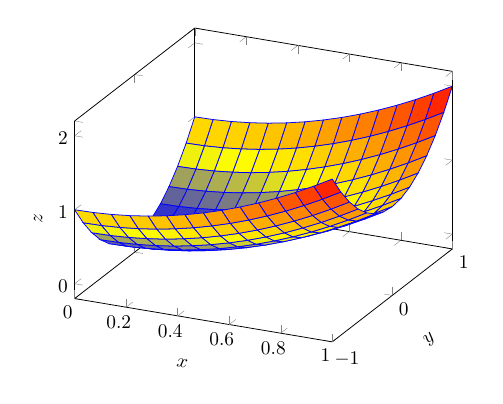
\begin{tikzpicture}[scale=.7]
		\begin{axis}[
			xlabel=$x$,
			ylabel=$y$,
			zlabel=$z$,
			xlabel style={sloped},
			ylabel style={sloped},
		]
			\addplot3[
				surf,
				faceted color=blue,
				samples=15,
				domain=0:1,y domain=-1:1
			]{x^2 + y^2};
		\end{axis}
	\end{tikzpicture}
	\caption{}
	\label{figure:解析几何.椭圆抛物面}
\end{figure}

\subsubsection{双曲抛物面}
方程\begin{equation}\label{equation:解析几何.双曲抛物面的一般方程}
	\frac{x^2}{p}-\frac{y^2}{q}=2z,
	\quad p,q>0
\end{equation}
表示的曲面称为\DefineConcept{双曲抛物面}或\DefineConcept{马鞍面}.
它的图形如\cref{figure:解析几何.双曲抛物面} 所示.
它具有下述性质:
\begin{enumerate}
	\item 对称性.
	\(Ozx\)平面和\(Oyz\)平面都是双曲抛物面的对称平面,\(z\)轴是它的对称轴.

	\item 形状.
	双曲抛物面与\(Oxy\)平面的交线为\[
		\left\{ \begin{array}{l}
			\frac{x^2}{p} - \frac{y^2}{q} = 0, \\
			z = 0.
		\end{array} \right.
	\]
	这时一对经过原点的相交直线.

	双曲抛物面与\(Ozx\)平面、\(Oyz\)平面的交线分别为\[
		\left\{ \begin{array}{l}
			x^2 = 2pz, \\
			y = 0,
		\end{array} \right.
		\qquad
		\left\{ \begin{array}{l}
			y^2 = -2qz, \\
			x = 0;
		\end{array} \right.
	\]
	它们都是抛物线.

	用平面\(z=h\ (h\neq0)\)去截此曲面,得到的截口为\[
		\left\{ \begin{array}{l}
			\frac{x^2}{p} - \frac{y^2}{q} = 2h, \\
			z = h.
		\end{array} \right.
	\]
	这是一条双曲线;
	当\(h>0\)时,它的实轴平行于\(x\)轴;
	当\(h<0\)时,它的实轴平行于\(y\)轴.

	当平行移动抛物线\[
		\left\{ \begin{array}{l}
			y^2 = -2qz, \\
			x = 0,
		\end{array} \right.
	\]
	使得它的顶点沿抛物线\[
		\left\{ \begin{array}{l}
			x^2 = 2pz, \\
			y = 0
		\end{array} \right.
	\]移动时,
	便得到马鞍面.
	这是因为,点\(M(x,y,z)\)在此轨迹上的充分必要条件是:
	\(M\)在以抛物线\[
		\left\{ \begin{array}{l}
			x^2 = 2pz, \\
			y = 0
		\end{array} \right.
	\]上的一个点\(M_0(x_0,y_0,z_0)\)为顶点,
	且轴平行于\(z\)轴,
	形状、开口与\[
		\left\{ \begin{array}{l}
			y^2 = -2qz, \\
			x = 0
		\end{array} \right.
	\]一样的抛物线上,即有\[
		\left\{ \begin{array}{l}
			x_0^2 = 2pz_0, \\
			y_0 = 0, \\
			y^2 = -2q(z-z_0), \\
			x = x_0;
		\end{array} \right.
	\]
	消去\(x_0,y_0,z_0\),得到\[
		y^2=-2q\left(z - \frac{x^2}{2p}\right),
	\]
	整理得\[
		\frac{x^2}{p} - \frac{y^2}{q} = 2z.
	\]
\end{enumerate}

\begin{figure}[ht]%双曲抛物面
	\centering
	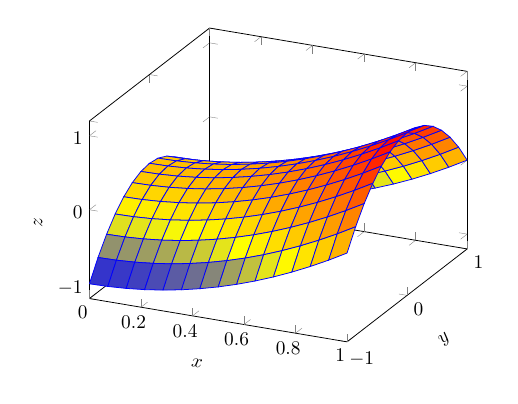
\begin{tikzpicture}[scale=.7]
		\begin{axis}[
			xlabel=$x$,
			ylabel=$y$,
			zlabel=$z$,
			xlabel style={sloped},
			ylabel style={sloped},
		]
			\addplot3[
				surf,
				faceted color=blue,
				samples=15,
				domain=0:1,y domain=-1:1
			]{x^2 - y^2};
		\end{axis}
	\end{tikzpicture}
	\caption{}
	\label{figure:解析几何.双曲抛物面}
\end{figure}

\subsubsection{二次曲面的种类}\label{section:解析几何.二次曲面的种类}
到目前为止,我们学过的二次曲面有以下17种:
\begin{enumerate}[label={\chinese*.}]
	\item 椭球面
	\begin{enumerate}[label={\arabic*.}]
		\item 椭球面:\[
			\frac{x^2}{a^2}+\frac{y^2}{b^2}+\frac{z^2}{c^2}=1;
		\]

		\item 虚椭球面:\[
			\frac{x^2}{a^2}+\frac{y^2}{b^2}+\frac{z^2}{c^2}=-1;
		\]

		\item 点:\[
			\frac{x^2}{a^2}+\frac{y^2}{b^2}+\frac{z^2}{c^2}=0;
		\]
	\end{enumerate}

	\item 双曲面
	\begin{enumerate}[label={\arabic*.}]
		\setcounter{enumii}{3}
		\item 单叶双曲面:\[
			\frac{x^2}{a^2}+\frac{y^2}{b^2}-\frac{z^2}{c^2}=1;
		\]

		\item 双叶双曲面:\[
			\frac{x^2}{a^2}+\frac{y^2}{b^2}-\frac{z^2}{c^2}=-1;
		\]
	\end{enumerate}

	\item 抛物面
	\begin{enumerate}[label={\arabic*.}]
		\setcounter{enumii}{5}
		\item 椭圆抛物面:\[
			\frac{x^2}{p}+\frac{y^2}{q}=2z;
		\]

		\item 双曲抛物面:\[
			\frac{x^2}{p}-\frac{y^2}{q}=2z;
		\]
	\end{enumerate}

	\item 二次锥面
	\begin{enumerate}[label={\arabic*.}]
		\setcounter{enumii}{7}
		\item 二次锥面:\[
			\frac{x^2}{a^2}+\frac{y^2}{b^2}-\frac{z^2}{c^2}=0;
		\]
	\end{enumerate}

	\item 二次柱面
	\begin{enumerate}[label={\arabic*.}]
		\setcounter{enumii}{8}
		\item 椭圆柱面:\[
			\frac{x^2}{a^2}+\frac{y^2}{b^2}=1;
		\]

		\item 虚椭圆柱面:\[
			\frac{x^2}{a^2}+\frac{y^2}{b^2}=-1;
		\]

		\item 直线:\[
			\frac{x^2}{a^2}+\frac{y^2}{b^2}=0;
		\]

		\item 双曲柱面:\[
			\frac{x^2}{a^2}-\frac{y^2}{b^2}=1;
		\]

		\item 一对相交平面:\[
			\frac{x^2}{a^2}-\frac{y^2}{b^2}=0;
		\]

		\item 抛物柱面:\[
			x^2=2py;
		\]

		\item 一对平行平面:\[
			x^2=a^2;
		\]

		\item 一对虚平行平面:\[
			x^2=-a^2;
		\]

		\item 一对重合平面:\[
			x^2=0.
		\]
	\end{enumerate}
\end{enumerate}
我们可以证明二次曲面只有这17种.

不过有的地方也只考虑以下9种曲面是二次曲面:
\begin{enumerate}
	\item 椭圆锥面
	\item 椭球面
	\item 单叶双曲面
	\item 双叶双曲面
	\item 椭圆抛物面
	\item 双曲抛物面
	\item 椭圆柱面
	\item 双曲柱面
	\item 抛物柱面
\end{enumerate}

\subsection{直纹面}
我们看到,柱面和锥面都是由直线组成的.
那么有没有别的也由直线组成的曲面呢?

\begin{definition}
给定一个曲面\(S\),如果存在一族直线,使得这一族中的每一条直线都在\(S\)上,
并且\(S\)上的每一个点都在这一族的某一条直线上,
那么我们称曲面\(S\)为\DefineConcept{直纹面},
称这一族直线为\(S\)的一族\DefineConcept{直母线}.
\end{definition}

二次曲面中哪些是直纹面呢?
9种二次曲面和1种二次锥面都是直纹面.
3种椭球面不是直纹面,因为它有界.
双叶双曲面不是直纹面,
因为当它由方程 \labelcref{equation:解析几何.双叶双曲面} 给出时,
平行于\(Oxy\)平面的直线不可能全在\(S\)上,
与\(Oxy\)平面相交的直线也不会全在\(S\)上.
同理可知,椭圆抛物面不是直纹面.
剩下的2种二次曲面,单叶双曲面和双曲抛物面,可以证明都是直纹面.

\begin{theorem}
单叶双曲面是直纹面.
\begin{proof}
设单叶双曲面\(S\)的方程是\[
	\frac{x^2}{a^2}+\frac{y^2}{b^2}-\frac{z^2}{c^2}=1.
\]
点\(M_0(x_0,y_0,z_0)\)在单叶双曲面\(S\)上的充分必要条件是\[
	\frac{x_0^2}{a^2}+\frac{y_0^2}{b^2}-\frac{z_0^2}{c^2}=1.
\]
移项并且分解因式,得\[
	\left(\frac{x_0}{a}+\frac{z_0}{c}\right)
	\left(\frac{x_0}{a}-\frac{z_0}{c}\right)
	= \left(1+\frac{y_0}{b}\right)
	\left(1-\frac{y_0}{b}\right),
\]
即\[
	\def\arraystretch{1.5}
	\begin{vmatrix}
		\frac{x_0}{a}+\frac{z_0}{c} & 1+\frac{y_0}{b} \\
		1-\frac{y_0}{b} & \frac{x_0}{a}-\frac{z_0}{c}
	\end{vmatrix} = 0.
\]
因为\(1\pm\frac{y_0}{b}\)不全为零,所以方程组\[
	\left\{ \def\arraystretch{1.5} \begin{array}{l}
		\left(\frac{x_0}{a}+\frac{z_0}{c}\right) X
		+ \left(1+\frac{y_0}{b}\right) Y = 0, \\
		\left(1-\frac{y_0}{b}\right) X
		+ \left(\frac{x_0}{a}-\frac{z_0}{c}\right) Y = 0
	\end{array} \right.
\]
是\(X,Y\)的一次齐次方程组.
如前所述,它的系数行列式为零,所以它有非零解,
即存在不全为零的实数\(\mu_0,\nu_0\),使得\[
	\left\{ \def\arraystretch{1.5} \begin{array}{l}
		\mu_0 \left(\frac{x_0}{a}+\frac{z_0}{c}\right)
		+ \nu_0 \left(1+\frac{y_0}{b}\right) = 0, \\
		\mu_0 \left(1-\frac{y_0}{b}\right)
		+ \nu_0 \left(\frac{x_0}{a}-\frac{z_0}{c}\right) = 0.
	\end{array} \right.
\]
这表明点\(M_0\)在直线\[
	l_0: \left\{ \def\arraystretch{1.5} \begin{array}{l}
		\mu_0 \left(\frac{x}{a}+\frac{z}{c}\right)
		+ \nu_0 \left(1+\frac{y}{b}\right) = 0, \\
		\mu_0 \left(1-\frac{y}{b}\right)
		+ \nu_0 \left(\frac{x}{a}-\frac{z}{c}\right) = 0
	\end{array} \right.
\]上.
现在考虑一族直线:\[
	\mathcal{L}:
	\left\{ \def\arraystretch{1.5} \begin{array}{l}
		\mu \left(\frac{x}{a}+\frac{z}{c}\right)
		+ \nu \left(1+\frac{y}{b}\right) = 0, \\
		\mu \left(1-\frac{y}{b}\right)
		+ \nu \left(\frac{x}{a}-\frac{z}{c}\right) = 0,
	\end{array} \right.
\]
其中\(\mu,\nu\)取所有不全为零的实数.
若\((\mu_1,\nu_1)\)与\((\mu_2,\nu_2)\)成比例,
则它们确定直线族\(\mathcal{L}\)中的同一条直线;
若它们不成比例,则它们确定不同的直线.
所以直线族\(\mathcal{L}\)实际上只依赖于一个参数,即\(\mu\)与\(\nu\)的比值.
上面就证明了:
单叶双曲面\(S\)上的任一点\(M_0\)在直线族\(\mathcal{L}\)的某一条直线\(l_0\)上.
现在从直线族\(\mathcal{L}\)中任取一条直线\(l_1\),它对应于\((\mu_1,\nu_1)\),
且在\(l_1\)上任取一点\(M_1(x_1,y_1,z_1)\),则有\[
	\left\{ \def\arraystretch{1.5} \begin{array}{l}
		\mu_1 \left(\frac{x_1}{a}+\frac{z_1}{c}\right)
		+ \nu_1 \left(1+\frac{y_1}{b}\right) = 0, \\
		\mu_1 \left(1-\frac{y_1}{b}\right)
		+ \nu_1 \left(\frac{x_1}{a}-\frac{z_1}{c}\right) = 0.
	\end{array} \right.
\]
因为\(\mu_1,\nu_1\)不全为零,所以上式说明方程组\[
	\left\{ \def\arraystretch{1.5} \begin{array}{l}
		\left(\frac{x_1}{a}+\frac{z_1}{c}\right) X
		+ \left(1+\frac{y_1}{b}\right) Y = 0, \\
		\left(1-\frac{y_1}{b}\right) X
		+ \left(\frac{x_1}{a}-\frac{z_1}{c}\right) Y = 0
	\end{array} \right.
\]有非零解,从而它的系数行列式等于零.
于是可知,\(M_1(x_1,y_1,z_1)\)在单叶双曲面\(S\)上,
也就是说,\(S\)是直纹面,且直线族\(\mathcal{L}\)是它的一族直母线.

考虑到\[
	\def\arraystretch{1.5}
	\begin{vmatrix}
		\frac{x_0}{a}+\frac{z_0}{c} & 1-\frac{y_0}{b} \\
		1+\frac{y_0}{b} & \frac{x_0}{a}-\frac{z_0}{c}
	\end{vmatrix}
	= \begin{vmatrix}
		\frac{x_0}{a}+\frac{z_0}{c} & 1+\frac{y_0}{b} \\
		1-\frac{y_0}{b} & \frac{x_0}{a}-\frac{z_0}{c}
	\end{vmatrix},
\]
我们还可以类似地得到\(S\)的另一族直母线\[
	\left\{ \def\arraystretch{1.5} \begin{array}{l}
		\mu \left(\frac{x}{a}+\frac{z}{c}\right)
		+ \nu \left(1-\frac{y}{b}\right) = 0, \\
		\mu \left(1+\frac{y}{b}\right)
		+ \nu \left(\frac{x}{a}-\frac{z}{c}\right) = 0,
	\end{array} \right.
\]
其中\(\mu,\nu\)取所有不全为零的实数.
\end{proof}
\end{theorem}

\begin{theorem}
双曲抛物面是直纹面.
\begin{proof}
设双曲抛物面\(S\)的方程是\[
	\frac{x^2}{p}-\frac{y^2}{q}=2z,
\]
则它有两族直母线\[
	\left\{ \def\arraystretch{1.5} \begin{array}{l}
		\left(\frac{x}{\sqrt{p}}+\frac{y}{\sqrt{q}}\right)+2\lambda=0, \\
		z+\lambda\left(\frac{x}{\sqrt{p}}-\frac{y}{\sqrt{q}}\right)=0
	\end{array} \right.
	\quad\text{和}\quad
	\left\{ \def\arraystretch{1.5} \begin{array}{l}
		\lambda\left(\frac{x}{\sqrt{p}}+\frac{y}{\sqrt{q}}\right)+z=0, \\
		2\lambda\left(\frac{x}{\sqrt{p}}-\frac{y}{\sqrt{q}}\right)=0,
	\end{array} \right.
\]
其中\(\lambda\)取所有实数.
\end{proof}
\end{theorem}


\subsection{曲面的交线,曲面围成的区域}
\subsubsection{画空间图形常见的三种方法}
在纸上描绘空间图形时,我们常用以下三种方法:
\begin{enumerate}
	\item 斜二测法(或称斜二等轴测投影法).
	让\(z\)轴垂直向上,\(y\)轴水平向右,
	\(x\)轴与\(y\)轴、\(z\)轴分别成 135\textdegree 角.
	规定\(y\)轴与\(z\)轴的单位长度相等,
	而\(x\)轴的单位长度为\(y\)轴单位长度的一半.

	\item 正等测法(即正等轴测投影法).
	让\(z\)轴垂直向上,
	\(x\)轴、\(y\)轴、\(z\)轴两两成 120\textdegree 角.
	规定三根轴的单位长度相等.

	\item 正二测法(即正二等轴测投影法).
	具体地说,有以下两种作图方案:
	\begin{itemize}
		\item 让\(z\)轴垂直向上,
		\(x\)轴与\(z\)轴的夹角为\(90^\circ + \alpha\),
		其中\(\alpha\)是锐角,且\(\tan\alpha\approx\frac{7}{8}\);
		\(y\)轴与\(z\)轴的夹角为\(90^\circ + \beta\),
		其中\(\beta\)是锐角,且\(\tan\beta\approx\frac{1}{8}\).
		规定\(z\)轴和\(y\)轴的单位长度相等,
		而\(x\)轴的单位长度为\(y\)轴的单位长度的一半.

		\item 仍然让\(z\)轴垂直向上,
		\(x\)轴与\(z\)轴夹角为\(90^\circ + \beta\),
		其中\(\tan\beta\approx\frac{1}{8}\);
		\(y\)轴的负向与\(z\)轴的夹角为\(90^\circ + \alpha\),
		其中\(\tan\alpha\approx\frac{7}{8}\).
		规定\(x\)轴与\(z\)轴的单位长度相等,
		\(y\)轴的单位长度为\(z\)轴的单位长度的一半.
	\end{itemize}
	一般来说,采用正二测法画出的图形较为逼真.
\end{enumerate}

\subsubsection{曲线在坐标平面上的投影,曲面的交线的画法}
如\cref{figure:解析几何.点在坐标平面上的投影},
对于空间中任一点\(M\)以及它在三个坐标平面上的投影点\(M_1,M_2,M_3\)这四个点,
只要知道了其中两个点就可以画出另外两个点.
譬如,若知道了\(M_2,M_3\)两个点,则只要分别过\(M_2,M_3\)画出投影线(平行于相应坐标轴的直线),
它们的交点就是点\(M\),再过\(M\)画投影线(平行于\(z\)轴),
它与\(Oxy\)平面的交点就是点\(M_1\).

\begin{figure}[ht]
	\centering
	\begin{tikzpicture}
		\def\spacecoordinate(#1,#2,#3,#4){\coordinate(#1)at(#3-#2*0.35355,#4-#2*0.35355);}%
		\spacecoordinate(O,0,0,0)
		\spacecoordinate(A,1,2,3)
		\spacecoordinate(A1,1,2,0)
		\spacecoordinate(A2,0,2,3)
		\spacecoordinate(A3,1,0,3)

		\begin{scope}[->]
			\draw(O)--(3,0)node[right]{\(y\)};
			\draw(O)--(0,4)node[right]{\(z\)};
			\draw(O)--(-1,-1)node[left]{\(x\)};
		\end{scope}
		\filldraw
			(O)node[above right]{\(O\)}
			(A)circle(2pt)node[right]{\(M\)}
			(A1)circle(2pt)node[right]{\(M_1\)}
			(A2)circle(2pt)node[right]{\(M_2\)}
			(A3)circle(2pt)node[left]{\(M_3\)};
		\draw[dashed]
			(A)--(A1)
			(A)--(A2)
			(A)--(A3);
	\end{tikzpicture}
	\caption{}
	\label{figure:解析几何.点在坐标平面上的投影}
\end{figure}

因此,为了画出两个曲面的交线\(\Gamma\),
只需要先画出\(\Gamma\)上每个点在某两个坐标面上的投影.
\(\Gamma\)上所有点在某个平面\(\alpha\)
(这个平面可以是\(Oxy\)平面、\(Oyz\)平面或\(Ozx\)平面)
上的投影组成的曲线,
称为“\(\Gamma\)在\(\alpha\)上的\DefineConcept{投影曲线}”,
简称为“\(\Gamma\)在\(\alpha\)上的\DefineConcept{投影}”.
如果我们把\(\alpha\)的法线记为\(l\),
把以\(\Gamma\)准线、母线平行于\(l\)的柱面记为\(S\),
那么曲线\(\Gamma\)在\(\alpha\)上的投影就是\(S\)与\(\alpha\)的交线,
我们称柱面\(S\)为“\(\Gamma\)沿\(l\)的\DefineConcept{投影柱面}”.

\subsubsection{曲面所围成的区域的画法}
几个曲面或平面所围成的空间的区域可用几个不等式联立起来表示.
如何画出这个区域呢?
关键是要画出相应曲面的交线,随之可得所求空间区域.

\section{坐标变换}
前两节我们再选定的一个坐标系中研究平面、直线和曲面.
但是,在许多情形下,往往在实现给定的坐标系中一个图形的方程比较复杂,
这时我们需要选择领一个合适的坐标系,使这个图形的方程变得比较简单.
为此,就需要研究同一个点在两个坐标系中的坐标之间的关系.
这样的关系式就称为\DefineConcept{坐标变换公式}.
我们在本节来研究坐标变换公式及其应用.

\subsection{平面的仿射坐标变换}
\subsubsection{点的仿射坐标变换公式}
平面上给了两个仿射坐标系:
\([O;\vb{d}_1,\vb{d}_2]\)
和\([O';\vb{d}_1',\vb{d}_2']\).
为方便起见,前一个称为旧坐标系,简记为 I;
后一个称为新坐标系,简记为 II.
点或向量在 I 中的坐标称为它的旧坐标,
在 II 中的坐标称为它的新坐标.
为了研究同一个点的新旧坐标的关系,
首先要明确上述两个坐标系的相对位置.

设 II 的原点\(O'\)的旧坐标是\((x_0,y_0)\),
基向量\(\vb{d}_1',\vb{d}_2'\)的旧坐标分别是\((a_{11},a_{21})\)和\((a_{12},a_{22})\).
现在我们来求某一点\(M\)的旧坐标\((x,y)\)与它的新坐标\((x',y')\)之间的关系.
因为\begin{align*}
	\vec{OM}
	&= \vec{O O'} + \vec{O' M}
	= (x_0 \vb{d}_1 + y_0 \vb{d}_2)
	+ (x' \vb{d}_1' + y' \vb{d}_2') \\
	&= (x_0 \vb{d}_1 + y_0 \vb{d}_2)
	+ x' (a_{11} \vb{d}_1 + a_{21} \vb{d}_2)
	+ y' (a_{12} \vb{d}_1 + a_{22} \vb{d}_2) \\
	&= (a_{11} x' + a_{12} y' + x_0) \vb{d}_1
	+ (a_{21} x' + a_{22} y' + y_0) \vb{d}_2,
\end{align*}
所以有\begin{equation}\label{equation:解析几何.平面坐标系的点的仿射坐标变换公式I到II}
	\left\{ \begin{array}{l}
		x = a_{11} x' + a_{12} y' + x_0, \\
		y = a_{21} x' + a_{22} y' + y_0.
	\end{array} \right.
\end{equation}
\cref{equation:解析几何.平面坐标系的点的仿射坐标变换公式I到II}
称为“平面上坐标系 I 到 II 的点的\DefineConcept{仿射坐标变换公式}”.
它是一个把任意一点\(M\)的旧坐标\(x,y\)表示成它的新坐标\(x',y'\)的一次多项式.

利用矩阵,我们可以将\cref{equation:解析几何.平面坐标系的点的仿射坐标变换公式I到II}
化为\begin{equation}\label{equation:解析几何.平面坐标系的点的仿射坐标变换公式I到II.矩阵形式1}
	\begin{bmatrix}
		x \\ y
	\end{bmatrix}
	= \begin{bmatrix}
		a_{11} & a_{12} \\
		a_{21} & a_{22}
	\end{bmatrix} \begin{bmatrix}
		x' \\ y'
	\end{bmatrix} + \begin{bmatrix}
		x_0 \\ y_0
	\end{bmatrix}.
\end{equation}
我们称矩阵\[
	\vb{A} = \begin{bmatrix}
		a_{11} & a_{12} \\
		a_{21} & a_{22}
	\end{bmatrix}
\]为“坐标 I 到 II 的\DefineConcept{过渡矩阵}”,
它的第一列是 II 的第一个基向量\(\vb{d}_1'\)的 I 坐标,
第二列是 II 的第二个基向量\(\vb{d}_2'\)的 I 坐标.

\begin{theorem}
平面上点的仿射坐标变换公式 \labelcref{equation:解析几何.平面坐标系的点的仿射坐标变换公式I到II}
中的系数行列式不等于零,即\[
	\begin{vmatrix}
		a_{11} & a_{12} \\
		a_{21} & a_{22}
	\end{vmatrix} \neq 0.
\]
\end{theorem}

根据上述定理,如果我们把\cref{equation:解析几何.平面坐标系的点的仿射坐标变换公式I到II}
看作关于\(x',y'\)的方程组,可以求得唯一解
\begin{equation}\label{equation:解析几何.平面坐标系的点的仿射坐标变换公式II到I}
	\left\{ \begin{array}{l}
		x' = \frac{1}{D} \begin{vmatrix}
			x - x_0 & a_{12} \\
			y - y_0 & a_{22}
		\end{vmatrix}, \\
		y' = \frac{1}{D} \begin{vmatrix}
			a_{11} & x - x_0 \\
			a_{21} & y - y_0
		\end{vmatrix}.
	\end{array} \right.
\end{equation}
其中\[
	D = \begin{vmatrix}
		a_{11} & a_{12} \\
		a_{21} & a_{22}
	\end{vmatrix}.
\]
\cref{equation:解析几何.平面坐标系的点的仿射坐标变换公式II到I}
是把平面上任意一点\(M\)的新坐标\(x',y'\)表示成它的旧坐标\(x,y\)的一次多项式,
我们称其为“平面上坐标系 II 到 I 的点的仿射坐标变换公式”.

\subsubsection{向量的仿射坐标变换公式}
现在我们来看平面上的向量\(\vb{m}\)的旧坐标\((u,v)\)与它的新坐标\((u',v')\)之间的关系.
设\(\vb{m}=\vec{M_1 M_2}\),
其中点\(M_i\)的旧坐标为\((x_i,y_i)\),新坐标为\((x_i',y_i')\ (i=1,2)\),
则有\begin{align*}
	u &= x_2 - x_1
	= (a_{11} x_2' + a_{12} y_2' + x_0)
	- (a_{11} x_1' + a_{12} y_1' + x_0) \\
	&= a_{11} (x_2' - x_1')
	+ a_{12} (y_2' - y_1')
	= a_{11} u' + a_{12} v', \\
	v &= y_2 - y_1
	= (a_{21} x_2' + a_{22} y_2' + y_0)
	- (a_{21} x_1' + a_{22} y_1' + y_0) \\
	&= a_{21} u' + a_{22} v',
\end{align*}
即\begin{equation}\label{equation:解析几何.平面坐标系的向量的仿射坐标变换公式I到II}
	\left\{ \begin{array}{l}
		u = a_{11} u' + a_{12} v', \\
		v = a_{21} u' + a_{22} v'.
	\end{array} \right.
\end{equation}
\cref{equation:解析几何.平面坐标系的向量的仿射坐标变换公式I到II}
称为“平面上坐标系 I 到 II 的向量的仿射坐标变换公式”.
它是把任意一个向量\(\vb{m}\)的旧坐标\(u,v\)表示成它的新坐标\(u',v'\)的一次齐次多项式,
这时与点的坐标变换公式不同的地方.
平面上的点和向量是有本质区别的两种对象,
如果只从一个坐标系来看,
似乎点和向量的坐标都是有序实数对,
看不出它们的区别;
但是,如果取两个原点不重合的仿射坐标系,
通过坐标变换,
就可以看出两者的显著区别:
点的坐标变换公式 \labelcref{equation:解析几何.平面坐标系的点的仿射坐标变换公式I到II} 中有常数项,
而向量的坐标变换公式 \labelcref{equation:解析几何.平面坐标系的向量的仿射坐标变换公式I到II} 中没有常数项.

利用矩阵,我们可以将\cref{equation:解析几何.平面坐标系的向量的仿射坐标变换公式I到II}
化为\begin{equation}\label{equation:解析几何.平面坐标系的向量的仿射坐标变换公式I到II.矩阵形式1}
	\begin{bmatrix}
		u \\ v
	\end{bmatrix}
	= \begin{bmatrix}
		a_{11} & a_{12} \\
		a_{21} & a_{22}
	\end{bmatrix} \begin{bmatrix}
		u' \\ v'
	\end{bmatrix}.
\end{equation}

由于\cref{equation:解析几何.平面坐标系的向量的仿射坐标变换公式I到II}
中的系数行列式仍然不为零,因此可以反解出
\begin{equation}\label{equation:解析几何.平面坐标系的向量的仿射坐标变换公式II到I}
	\left\{ \begin{array}{l}
		u' = \frac{1}{D} \begin{vmatrix}
			u & a_{12} \\
			v & a_{22}
		\end{vmatrix}, \\
		v' = \frac{1}{D} \begin{vmatrix}
			a_{11} & u \\
			a_{21} & v
		\end{vmatrix}.
	\end{array} \right.
\end{equation}
这是“平面上坐标系 II 到 I 的向量的仿射坐标变换公式”.
由\cref{equation:解析几何.平面坐标系的向量的仿射坐标变换公式II到I} 看出,
I 的基向量\(\vb{d}_1,\vb{d}_2\)的 II 坐标分别是\[
	\frac{1}{D} (a_{22},-a_{21}), \qquad
	\frac{1}{D} (-a_{12},a_{11}).
\]

\subsection{平面的直角坐标变换}
设 I \([O;\vb{e}_1,\vb{e}_2]\),II \([O';\vb{e}_1',\vb{e}_2']\)都是直角坐标系.
前一小节关于仿射坐标变换的一般结论和方法对于直角坐标变换都成立,
也就是说我们其实也可以直接应用\cref{%
equation:解析几何.平面坐标系的点的仿射坐标变换公式I到II,%
equation:解析几何.平面坐标系的点的仿射坐标变换公式II到I,%
equation:解析几何.平面坐标系的向量的仿射坐标变换公式I到II,%
equation:解析几何.平面坐标系的向量的仿射坐标变换公式II到I}
进行直角坐标变换.
不过,由于直角坐标系的特殊性,
我们可以对平面上坐标系 II 到 I 的点(或向量)的坐标变换公式进行简化.

\subsubsection{直角坐标变换公式}
设\(O'\)的 I 坐标为\((x_0,y_0)\),
\(\vb{e}_1',\vb{e}_2'\)的 I 坐标分别为\((a_{11},a_{21}),(a_{12},a_{22})\),
则坐标系 I 到 II 的过渡矩阵是\[
	\vb{A} = \begin{bmatrix}
		a_{11} & a_{12} \\
		a_{21} & a_{22}
	\end{bmatrix}.
\]

\begin{theorem}\label{theorem:解析几何.直角坐标变换的过渡矩阵是正交矩阵}
设 I 和 II 都是直角坐标系,
则 I 到 II 的过渡矩阵\(\vb{A}\)是正交矩阵,
并且坐标系 II 到 I 的过渡矩阵是\(\vb{A}^T\).
\begin{proof}
因为\(\abs{\vb{e}_1'}=\abs{\vb{e}_2'}=1\),
\(\vb{e}_1' \perp \vb{e}_2'\),
并且 I 是直角坐标系,
所以有\begin{equation}\label{equation:解析几何.直角坐标变换的过渡矩阵的限定条件}
	\left\{ \begin{array}{l}
		a_{11}^2 + a_{21}^2 = 1, \\
		a_{12}^2 + a_{22}^2 = 1, \\
		a_{11} a_{12} + a_{21} a_{22} = 0.
	\end{array} \right.
\end{equation}
于是\(\vb{A}\)是正交矩阵.
\end{proof}
\end{theorem}

现在依据\cref{theorem:解析几何.直角坐标变换的过渡矩阵是正交矩阵},
我们可以将\cref{equation:解析几何.平面坐标系的点的仿射坐标变换公式II到I,%
equation:解析几何.平面坐标系的向量的仿射坐标变换公式II到I} 改为计算相对简单的以下两个公式:
\begin{equation}\label{equation:解析几何.平面坐标系的点的直角坐标变换公式II到I.矩阵形式1}
	\begin{bmatrix}
		x' \\ y'
	\end{bmatrix}
	= \begin{bmatrix}
		a_{11} & a_{21} \\
		a_{12} & a_{22}
	\end{bmatrix} \begin{bmatrix}
		x - x_0 \\ y - y_0
	\end{bmatrix},
\end{equation}
\begin{equation}\label{equation:解析几何.平面坐标系的向量的直角坐标变换公式II到I.矩阵形式1}
	\begin{bmatrix}
		u' \\ v'
	\end{bmatrix}
	= \begin{bmatrix}
		a_{11} & a_{21} \\
		a_{12} & a_{22}
	\end{bmatrix} \begin{bmatrix}
		u \\ v
	\end{bmatrix}.
\end{equation}

\subsubsection{直角坐标变换的过渡矩阵}
直角坐标系 I 到 II 的过渡矩阵\(\vb{A}\)虽然有四个数,
但是由于它是正交矩阵,
满足\cref{equation:解析几何.直角坐标变换的过渡矩阵的限定条件} 中的三个方程,
因此只有一个数是自由的.
下面来详细讨论这一点.

给定平面上的仿射坐标系\([O;\vb{d}_1,\vb{d}_2]\),
如果从\(\vb{d}_1\)逆时针旋转小于 180\textdegree 的角便与\(\vb{d}_2\)重合,
则称这个坐标系为右手坐标系,简称右手系;
反之,则称之为左手坐标系,简称左手系.
特别地,对于直角坐标系\([O;\vb{e}_1,\vb{e}_2]\)来说,
若\(\vb{e}_1\)旋转 90\textdegree 与\(\vb{e}_2\)重合,则为右手系;
若\(\vb{e}_1\)旋转 -90\textdegree 与\(\vb{e}_2\)重合,则为左手系.

设 I \([O;\vb{e}_1,\vb{e}_2]\),II \([O';\vb{e}_1',\vb{e}_2']\)都是右手直角坐标系,且\[
	O'(x_0,y_0), \qquad
	\vb{e}_1'(a_{11},a_{21}), \qquad
	\vb{e}_2'(a_{12},a_{22}),
\]则有{\def\ExprA#1#2{a_{#1#2} = \vb{e}_#2' \cdot \vb{e}_#1 = \cos\angle(\vb{e}_#2',\vb{e}_#1)}
\begin{align*}
	\ExprA{1}{1}, \qquad
	\ExprA{2}{1}, \\
	\ExprA{1}{2}, \qquad
	\ExprA{2}{2}.
\end{align*}}

\begin{figure}[ht]
	\centering
	\begin{tikzpicture}[->,scale=2]
		\draw(0,0)node[below left]{\(O\)}--(1,0)node[right]{\(\vb{e}_1\)};
		\draw(0,0)--(0,1)node[left]{\(\vb{e}_2\)};
		\begin{scope}[xshift=1.3cm,yshift=1.3cm]
			\draw[dashed,-](0,1)coordinate(E2)--(0,0)coordinate(O)node[below left]{\(O'\)}--(1,0)coordinate(E1);
			\draw(0,0)--(.866,.5)coordinate(E11)node[above right]{\(\vb{e}_1'\)};
			\draw(0,0)--(-.5,.866)coordinate(E22)node[above left]{\(\vb{e}_2'\)};
			\draw pic["\(\theta\)",draw=orange,-,angle eccentricity=1.7,angle radius=5mm]{angle=E1--O--E11};
			\draw pic[draw=orange,-,angle radius=5mm]{angle=E2--O--E22};
		\end{scope}
	\end{tikzpicture}
	\caption{}
	\label{figure:解析几何.平面坐标变换的过渡矩阵与旋转角的关系}
\end{figure}

如\cref{figure:解析几何.平面坐标变换的过渡矩阵与旋转角的关系},
设\(\vb{e}_1\)逆时针旋转\(\theta\)角便与\(\vb{e}_1'\)重合,
在\[
	0 \leq \theta < \frac{\pi}{2}, \qquad
	\frac{\pi}{2} \leq \theta < \pi, \qquad
	\pi \leq \theta < \frac{3}{2}\pi, \qquad
	\frac{3}{2}\pi \leq \theta < 2\pi
\]这四种情况下,总可得\[
	a_{11} = \cos\theta, \qquad
	a_{21} = \sin\theta, \qquad
	a_{12} = -\sin\theta, \qquad
	a_{22} = \cos\theta,
\]
那么 I 到 II 的过渡矩阵为\[
	\vb{A} = \begin{bmatrix}
		\cos\theta & -\sin\theta \\
		\sin\theta & \cos\theta
	\end{bmatrix}.
\]
应该注意到,\(\abs{\vb{A}}=1\).

类似地,设\(\theta\)仍表示\(\vb{e}_1\)到\(\vb{e}_1'\)的转角,
若 I 是右手直角坐标系,而 II 是左手直角坐标系,
则 I 到 II 的过渡矩阵为\[
	\begin{bmatrix}
		\cos\theta & \sin\theta \\
		\sin\theta & -\cos\theta
	\end{bmatrix};
\]
若 I 是左手直角坐标系,而 II 是右手直角坐标系,
则 I 到 II 的过渡矩阵为\[
	\begin{bmatrix}
		\cos\theta & -\sin\theta \\
		-\sin\theta & -\cos\theta
	\end{bmatrix};
\]
若 I 和 II 都是左手直角坐标系,
则 I 到 II 的过渡矩阵为\[
	\begin{bmatrix}
		\cos\theta & \sin\theta \\
		-\sin\theta & \cos\theta
	\end{bmatrix}.
\]

\begin{definition}
给定平面(或空间)的两个坐标系,
如果它们都是右手系,或者它们都是左手系,
则称它们是\DefineConcept{同定向的};
如果一个是左手系,另一个是右手系,
则称它们是\DefineConcept{反定向的}.
\end{definition}

从上面的讨论可以得到
\begin{theorem}
设 I 和 II 都是平面的直角坐标系,
I 到 II 的过渡矩阵是\(\vb{A}\),
则 I 和 II 同定向的充分必要条件是\(\abs{\vb{A}}=1\),
从而它们反定向的充分必要条件是\(\abs{\vb{A}}=-1\).
\end{theorem}

如无特别声明,今后所取的直角坐标系都是右手系.

\subsubsection{移轴公式和转轴公式}
设 I \([O;\vb{e}_1,\vb{e}_2]\),II \([O';\vb{e}_1',\vb{e}_2']\)都是右手直角坐标系,
\(O'(x_0,y_0)\),
\(\vb{e}_1\)到\(\vb{e}_1'\)的转角为\(\theta\),
则 I 到 II 的点的坐标变换公式为
\begin{equation}\label{equation:解析几何.平面坐标系的点的右手直角坐标变换公式I到II.矩阵形式1}
	\begin{bmatrix}
		x \\ y
	\end{bmatrix} = \begin{bmatrix}
		\cos\theta & -\sin\theta \\
		\sin\theta & \cos\theta
	\end{bmatrix} \begin{bmatrix}
		x' \\ y'
	\end{bmatrix} + \begin{bmatrix}
		x_0 \\ y_0
	\end{bmatrix}.
\end{equation}

若\(\theta=0\),
则\cref{equation:解析几何.平面坐标系的点的右手直角坐标变换公式I到II.矩阵形式1} 成为
\begin{equation}\label{equation:解析几何.平面坐标系的点的右手直角坐标变换公式I到II.矩阵形式2}
	\begin{bmatrix}
		x \\ y
	\end{bmatrix} = \begin{bmatrix}
		1 & 0 \\
		0 & 1
	\end{bmatrix} \begin{bmatrix}
		x' \\ y'
	\end{bmatrix} + \begin{bmatrix}
		x_0 \\ y_0
	\end{bmatrix},
\end{equation}
即\begin{equation}\label{equation:解析几何.平面坐标系的点的右手直角坐标变换公式I到II.代数形式2}
	\left\{ \begin{array}{l}
		x = x' + x_0, \\
		y = y' + y_0.
	\end{array} \right.
\end{equation}
\cref{equation:解析几何.平面坐标系的点的右手直角坐标变换公式I到II.矩阵形式2,%
equation:解析几何.平面坐标系的点的右手直角坐标变换公式I到II.代数形式2}
称为\DefineConcept{移轴公式}.

若\(O'\)与\(O\)重合,
则\cref{equation:解析几何.平面坐标系的点的右手直角坐标变换公式I到II.矩阵形式1} 成为
\begin{equation}\label{equation:解析几何.平面坐标系的点的右手直角坐标变换公式I到II.矩阵形式3}
	\begin{bmatrix}
		x \\ y
	\end{bmatrix} = \begin{bmatrix}
		1 & 0 \\
		0 & 1
	\end{bmatrix} \begin{bmatrix}
		x' \\ y'
	\end{bmatrix}.
\end{equation}
\cref{equation:解析几何.平面坐标系的点的右手直角坐标变换公式I到II.矩阵形式3}
称为\DefineConcept{转轴公式}.

\cref{equation:解析几何.平面坐标系的点的右手直角坐标变换公式I到II.矩阵形式1,%
equation:解析几何.平面坐标系的点的右手直角坐标变换公式I到II.矩阵形式2,%
equation:解析几何.平面坐标系的点的右手直角坐标变换公式I到II.矩阵形式3}
说明,平面上任一右手直角坐标变换可以经过移轴和转轴得到,
即对于右手直角坐标系 I \([O;\vb{e}_1,\vb{e}_2]\) 和 II \([O';\vb{e}_1',\vb{e}_2']\),有\[
	[O;\vb{e}_1,\vb{e}_2]
	\xlongrightarrow{\text{移轴}}
	[O';\vb{e}_1,\vb{e}_2]
	\xlongrightarrow{\text{转轴}}
	[O';\vb{e}_1',\vb{e}_2']
\]或\[
	[O;\vb{e}_1,\vb{e}_2]
	\xlongrightarrow{\text{转轴}}
	[O;\vb{e}_1',\vb{e}_2']
	\xlongrightarrow{\text{移轴}}
	[O';\vb{e}_1',\vb{e}_2'].
\]

上述结论对于任意两个同定向的直角坐标系仍成立,但对于反定向的两个直角坐标系不成立.

\subsection{空间的仿射坐标变换}
\begin{theorem}\label{theorem:解析几何.空间的仿射坐标变换公式}
设 I \([O;\vb{d}_1,\vb{d}_2,\vb{d}_3]\)
和 II \([O';\vb{d}_1',\vb{d}_2',\vb{d}_3']\)
都是空间仿射坐标系,
\(O'\)的 I 坐标是\((x_0,y_0,z_0)\),
\(\vb{d}_j'\)的 I 坐标是\((a_{1j},a_{2j},a_{3j})\ (j=1,2,3)\),
则 I 到 II 的点的仿射坐标变换公式为
\begin{equation}
	\begin{bmatrix}
		x \\ y \\ z
	\end{bmatrix} = \begin{bmatrix}
		a_{11} & a_{12} & a_{13} \\
		a_{21} & a_{22} & a_{23} \\
		a_{31} & a_{32} & a_{33}
	\end{bmatrix} \begin{bmatrix}
		x' \\ y' \\ z'
	\end{bmatrix} + \begin{bmatrix}
		x_0 \\ y_0 \\ z_0
	\end{bmatrix},
\end{equation}
I 到 II 的向量的仿射坐标变换公式为
\begin{equation}
	\begin{bmatrix}
		u_1 \\ u_2 \\ u_3
	\end{bmatrix} = \begin{bmatrix}
		a_{11} & a_{12} & a_{13} \\
		a_{21} & a_{22} & a_{23} \\
		a_{31} & a_{32} & a_{33}
	\end{bmatrix} \begin{bmatrix}
		u_1' \\ u_2' \\ u_3'
	\end{bmatrix},
\end{equation}
其中\[
	\vb{A} = \begin{bmatrix}
		a_{11} & a_{12} & a_{13} \\
		a_{21} & a_{22} & a_{23} \\
		a_{31} & a_{32} & a_{33}
	\end{bmatrix}
\]称为“I 到 II 的过渡矩阵”,
它的第\(j\)列是\(\vb{d}_j'\ (j=1,2,3)\)的 I 坐标.
\end{theorem}

\begin{theorem}\label{theorem:解析几何.空间仿射坐标系同定向的充分必要条件}
仿射坐标系 I \([O;\vb{d}_1,\vb{d}_2,\vb{d}_3]\)
到 II \([O';\vb{d}_1',\vb{d}_2',\vb{d}_3']\)的过渡矩阵\(\vb{A}\)是非奇异的,
并且 I 与 II 同定向的充分必要条件是\(\abs{A}>0\).
\end{theorem}

\begin{corollary}
平面上的两个仿射坐标系 I \([O;\vb{d}_1,\vb{d}_2]\)
和 II \([O';\vb{d}_1',\vb{d}_2']\)同定向的充分必要条件是:
I 到 II 的过渡矩阵\(\vb{A}\)的行列式\(\abs{A}>0\).
\end{corollary}

\subsection{空间的直角坐标变换}
\cref{theorem:解析几何.空间的仿射坐标变换公式,%
theorem:解析几何.空间仿射坐标系同定向的充分必要条件}
在直角坐标系中当然也成立,
现在我们进一步研究直角坐标变换的特殊性.

\begin{theorem}
设 I \([O;\vb{e}_1,\vb{e}_2,\vb{e}_3]\)
和 II \([O';\vb{e}_1',\vb{e}_2',\vb{e}_3']\)
都是直角坐标系,
则 I 到 II 的过渡矩阵\(\vb{A}\)是正交矩阵,
从而 II 到 I 的过渡矩阵是\(\vb{A}^T\).
\end{theorem}

由于正交矩阵的行列式等于\(\pm1\),
因此空间的两个直角坐标系同定向的充分必要条件就是它们的过渡矩阵的行列式等于\(+1\).

\subsection{代数曲面、代数曲线及其次数}
空间(或平面)的任一点对于不同不同坐标系的坐标是不同的,
因而作为点的轨迹的图形在不同坐标系中的方程也就不同,但是有
\begin{theorem}\label{theorem:解析几何.坐标变换时代数图形的不变性}
若图形\(S\)在仿射坐标系 I 中的方程\(F(x,y,z)=0\)的左端是关于\(x,y,z\)的\(n\)次多项式,
则\(S\)在任意一个仿射坐标系 II 中的方程\(G(x',y',z')=0\)的左端是关于\(x',y',z'\)的\(n\)次多项式.
\end{theorem}
\cref{theorem:解析几何.坐标变换时代数图形的不变性} 说明,
一个图形的方程的左端是否为多项式,以及这个多项式的次数与坐标系的选择无关,
它们都是图形本身的性质.

若图形\(S\)的左端是多项式,则称\(S\)为\DefineConcept{代数曲面},
并且把这个多项式的次数称为这个代数曲面的\DefineConcept{次数}.

平面上的图形有类似的性质.
若平面上图形\(S\)的方程\(F(x,y)=0\)的左端是多项式,
则称\(S\)是\DefineConcept{代数曲线},
并且把这个多项式的次数称为这个代数曲线的\DefineConcept{次数}.
例如,椭圆、双曲线、抛物线在直角坐标系中的标准方程是二次的,
由此可知,它们不论在哪一个仿射坐标系中的方程也都是二次的,
所以它们才都被称为二次曲线.


\section{本章总结}
\subsection*{向量及其运算}
\begin{table}[ht]
	\centering
	\begin{tabular}{|c|c|c|c|}
	\hline
	\multicolumn{2}{|c|}{加法} & \multicolumn{2}{c|}{数乘} \\ \hline
	交换律 & \(\vb{a}+\vb{b}=\vb{b}+\vb{a}\) &
		结合律 & \(\lambda(\mu\vb{a})=\mu(\lambda\vb{a})=(\lambda\mu)\vb{a}\) \\ \hline
	\multirow{2}{*}{结合律} & \multirow{2}{*}{\((\vb{a}+\vb{b})+\vb{c}=\vb{a}+(\vb{b}+\vb{c})\)} &
		\multirow{2}{*}{分配律} & \((\lambda+\mu)\vb{a}=\lambda\vb{a}+\mu\vb{a}\) \\
	 & & & \(\lambda(\vb{a}+\vb{b})=\lambda\vb{a}+\lambda\vb{b}\) \\ \hline
	\multicolumn{2}{|c|}{点乘} & \multicolumn{2}{c|}{叉乘} \\ \hline
	交换律 & \(\vb{a}\cdot\vb{b}=\vb{b}\cdot\vb{a}\) &
		负交换律 & \(\vb{a}\times\vb{b}=-\vb{b}\times\vb{a}\) \\ \hline
	分配律 & \((\vb{a}+\vb{b})\cdot\vb{c}=\vb{a}\cdot\vb{c}+\vb{b}\cdot{c}\) &
		分配律 & \((\vb{a}+\vb{b})\times\vb{c}=\vb{a}\times\vb{c}+\vb{b}\times\vb{c}\) \\ \hline
	\multirow{3}{*}{结合律} & \((\lambda\vb{a})\cdot\vb{b}=\lambda(\vb{a}\cdot\vb{b})\) & \multirow{3}{*}{结合律} & \multirow{3}{*}{\((\lambda\vb{a})\times\vb{b}=\vb{a}\times(\lambda\vb{b})=\lambda(\vb{a}\times\vb{b})\)} \\
		& \(\vb{a}\cdot(\lambda\vb{b})=\lambda(\vb{a}\cdot\vb{b})\) & & \\
		& \((\lambda\vb{a})\cdot(\mu\vb{b})=\lambda\mu(\vb{a}\cdot\vb{b})\) & & \\
	\hline
	\end{tabular}
	\caption{向量的运算法则}
\end{table}

\subsection*{常见的坐标系}
极坐标系是一种平面坐标系.
极坐标系上的点\((\rho,\theta)\)与平面直角坐标系上的点\((x,y)\)存在以下的一一对应关系:\[
\left\{ \begin{array}{l}
x = \rho\cos\theta, \\
y = \rho\sin\theta. \\
\end{array} \right.
\]

柱面坐标系是一种空间坐标系.
柱面坐标系上的点\((\rho,\theta,z)\)与空间直角坐标系上的点\((x,y,z)\)存在以下的一一对应关系:\[
\left\{ \begin{array}{l}
x = \rho\cos\theta, \\
y = \rho\sin\theta, \\
z = z. \\
\end{array} \right.
\]

球极坐标系是一种空间坐标系.
球极坐标系上的点\((r,\theta,\phi)\)与空间直角坐标系上的点\((x,y,z)\)存在以下的一一对应关系:\[
\left\{ \begin{array}{l}
x = r \sin\phi \cos\theta, \\
y = r \sin\phi \sin\theta, \\
z = r \cos\phi. \\
\end{array} \right.
\]

\begin{figure}[h]
	\centering
	\begin{tikzpicture}
		\coordinate (O) at (0,0);
		\coordinate (M) at (2,2);
		\coordinate (P) at (2,-1.2);
		\coordinate (A) at (-0.8,-1.2);
		\coordinate (Z) at (0,1);
		\draw (O)node[left]{\(O\)}
				-- (M)node[right]{\(M\)} node[midway,above]{\(r\)}
				-- (P)node[right]{\(P\)} node[midway,right]{\(z\)}
				-- (A)node[left]{\(A\)} node[midway,below]{\(y\)}
				-- (O)node[midway,left]{\(x\)}
			(O) -- (P)
			pic["\(\phi\)",draw=orange,<-,angle eccentricity=1.3,angle radius=0.6cm]{angle=M--O--Z}
			pic["\(\theta\)",draw=orange,->,angle eccentricity=1.5,angle radius=0.4cm]{angle=A--O--P};
		\begin{scope}[>=Stealth,->,ultra thick]
			\draw(0,0) -- (-1.5,-2.25) node[right]{\(x\)};
			\draw(0,0) -- (3,0) node[right]{\(y\)};
			\draw(0,0) -- (0,3) node[above]{\(z\)};
		\end{scope}
	\end{tikzpicture}
	\caption{球极坐标系}
\end{figure}

\subsection*{常见二次曲面}
具体见\pagecref{section:解析几何.二次曲面的种类}.
